\section{Experiments} \label{experiments}
The conducted experiments involve many parameters that can be varied and combined to observe KENN's behavior from several points of view. The space of parameters is the following:
\begin{itemize}
    \item \textbf{KB mode:} the KB encoding strategy used to define the logical knowledge
    \item \textbf{initial clause weight:} the value used to initialize the network parameters of the clause weights
    \item \textbf{fixed/learnable clause weights:} the strategy used to set the clause weights
    \item \textbf{encoder:} the language model used to encode the textual input
    \item \textbf{loss function:} the loss function used during training
\end{itemize}
Before describing the experiments, we will introduce in the next sections the ET metrics and the training setups adopted. It is also important to point out that every model used the same initialization of random seeds, which guarantees: 
\begin{enumerate}
    \item Same layer initialization between different setups
    \item Given an epoch, each model is trained on the same batch of data
\end{enumerate}



\subsection{Metrics for Entity Typing}
The evaluation of an ET approach relies on some variants of the metrics used in classical classification problems. The explanation of each metric will be supported by numerical values obtained from the example in Table~\ref{tab:metrics_example}. 

\begin{table}[H]
\centering
\caption{Example of predictions over a type set $T=\{T1, T2, T3\}$ and a dataset $X=\{X1, X2, X3\}$}
\label{tab:metrics_example}
\begin{tabular}{c|ccc|ccc|}
\cline{2-7}
                                       & \multicolumn{3}{c|}{\textbf{Prediction}}                                          & \multicolumn{3}{c|}{\textbf{Target}}                                              \\ \hline
\multicolumn{1}{|c|}{\textbf{Example}} & \multicolumn{1}{c|}{\textbf{T1}} & \multicolumn{1}{c|}{\textbf{T2}} & \textbf{T3} & \multicolumn{1}{c|}{\textbf{T1}} & \multicolumn{1}{c|}{\textbf{T2}} & \textbf{T3} \\ \hline
\multicolumn{1}{|c|}{X$_{1}$}          & x                                &                                  & x           & x                                & x                                &             \\ \hline
\multicolumn{1}{|c|}{X$_{2}$}          &                                  & x                                &             & x                                &                                  & x           \\ \hline
\multicolumn{1}{|c|}{X$_{3}$}          & x                                &                                  & x           & x                                &                                  & x           \\ \hline
\end{tabular}
\end{table}

In the definition of the metrics we will use terminology that needs a preliminary explanation:
\begin{itemize}
    \item True Positive (\textbf{TP}): number of correct positive predictions. In the example in Table~\ref{tab:metrics_example} we have TP=3 .
    \item False Positive (\textbf{FP}): number of wrong positive predictions. In the example in Table~\ref{tab:metrics_example} we have FP=2 .
    \item True Negative (\textbf{TN}): number of correct negative predictions. In the example in Table~\ref{tab:metrics_example} we have TN=1 .
    \item False Negative (\textbf{FN}): number of wrong negative predictions. In the example in Table~\ref{tab:metrics_example} we have FN=3 .
\end{itemize}

Once fixed these preliminary notions, the evaluated metrics are defined as follows:

\begin{itemize}
    \item \textbf{Accuracy:} percentage of correct predictions; defined as 
    \begin{gather*}
        \frac{count(Prediction == Target)}{|X|} = \frac{1}{3}
    \end{gather*}
    
    \item \textbf{Micro precision:} percentage of correct positive predictions with respect to all the positive predictions; defined as
    \begin{gather*}
        \frac{TP}{TP + FP} = \frac{3}{3 + 2} = 0.6
    \end{gather*}
    
    \item \textbf{Micro recall:} percentage of correct positive predictions with respect to the positive target; defined as
    \begin{gather*}
        \frac{TP}{TP + FN} = \frac{3}{3 + 3} = 0.5
    \end{gather*}
    
    \item \textbf{Micro f1:} harmonic mean of micro precision and micro recall; defined as
    \begin{gather*}
        2 \cdot \frac{MicroPrecision \cdot MicroRecall}{MicroPrecision + MicroRecall} =
        2 \cdot \frac{0.6 \cdot 0.5}{0.6 + 0.5} = 0.54
    \end{gather*}
    
    \item \textbf{Macro precision examples:} mean of the percentages of correct positive predictions with respect to all the positive predictions of each example; defined as
    \begin{gather*}
        \frac{\sum_{x \in X}\frac{TP(x)}{TP(x) + FP(x)}}{|X|}=
        \frac{0.5 + 0 + 1}{3}=0.5
    \end{gather*}
    
    \item \textbf{Macro recall examples:} mean of the percentages of correct positive predictions with respect to the positive target of each example; defined as
    \begin{gather*}
        \frac{\sum_{x \in X}\frac{TP(x)}{TP(x) + FN(x)}}{|X|}=
        \frac{0.5 + 0 + 1}{3}=0.5
    \end{gather*}
    
    \item \textbf{Macro f1 examples:} harmonic mean of micro precision examples and micro recall examples; defined as
    \begin{gather*}
        2 \cdot \frac{MacroPrecisionExamples \cdot MacroRecallExamples}{MacroPrecisionExamples + MacroRecallExamples} =\\
        = 2 \cdot \frac{0.5 \cdot 0.5}{0.5 + 0.5} = 0.5
    \end{gather*}
    
    \item \textbf{Macro precision classes:} mean of the percentages of correct positive predictions with respect to all the positive predictions of each class; defined as
    \begin{gather*}
        \frac{\sum_{t \in T}\frac{TP(t)}{TP(t) + FP(t)}}{|T|} =
        \frac{1 + 0 + 0.5}{3} = 0.5
    \end{gather*}
    
    \item \textbf{Macro recall classes:} mean of the percentages of correct positive predictions with respect to the positive target of each class; defined as
    \begin{gather*}
        \frac{\sum_{t \in T}\frac{TP(t)}{TP(t) + FN(t)}}{|T|} =
        \frac{0.66 + 0 + 0.5}{3} = 0.38
    \end{gather*}
    
    \item \textbf{Macro f1 classes:} harmonic mean of macro precision classes and macro recall classes; defined as
    \begin{gather*}
        2 \cdot \frac{MacroPrecisionClasses \cdot MacroRecallClasses}{MacroPrecisionClasses + MacroRecallClasses} = \\
        = 2 \cdot \frac{0.5 \cdot 0.38}{0.5 + 0.38} = 0.43
    \end{gather*}
\end{itemize}
% \pagebreak
\subsection{Experimental setups}
Two setups were adopted for the experiments. The main differences between the setups are the stopping criterion and the batch size. In particular, \textit{Setup B} is used when BERT is involved since \textit{Setup A} would be too expensive.
\paragraph{Setup A} 
\begin{itemize}
    \item \textbf{number of epochs:} 100 for FIGER, 75 for BBN\footnote{BBN is smaller than FIGER and converges faster}
    \item \textbf{number of examples per epoch:} 10,240 (20 batches\footnote{using $n$ batches per epoch means performing $n$ backward operations per epoch} of size 512)
    \item \textbf{data shuffle:} each time the whole dataset has been seen
    \item \textbf{optimizer:} Adam with fixed learning rate set to 0.0005
    \item \textbf{inference:} threshold = 0.5
\end{itemize}

\paragraph{Setup B} 
\begin{itemize}
    \item \textbf{number of epochs:} undefined; determined by an early stopping strategy on the \textit{dev loss} with \textit{patience = 5}
    \item \textbf{number of examples per epoch:} 10,240 (160 batches of size 64)
    \item \textbf{data shuffle:} every time the whole dataset has been seen
    \item \textbf{optimizer:} Adam with fixed learning rate set to 0.0005
     \item \textbf{inference:} threshold = 0.5
\end{itemize}


\subsection{Baseline hyperparameter search}
The architecture of the baseline neural network was kept simple to have a basic starting point, so it did not involve any search of the best combination of hidden layers/units. The optimization aimed to find the best representation of the input text in terms of tokens and involved a few hyperparameters.


Fixed the training configuration following the \textit{Setup A}, we can proceed with the explanation of the hyperparameter search. We saw in section \ref{baseline_model} that the input of the model is split in mention, left context and right context tokens separated by \verb|[SEP]|. Although keeping every token of every span would feed the model with the maximum amount of information, this is not a feasible solution because of the high cost. For this reason, it is necessary to find the optimal number of tokens for both mention and context to reach a trade-off between cost and performance. Before going on, an important remark: tokens and words are two distinct things. In this case, we are looking for the optimal number of words that will be transformed by the tokenizer into a different number of tokens. Since BERT's tokenization is based on the WordPiece, the number of tokens grows up rapidly due to the subwords segmentation. For this reason, the maximum number of tokens is capped to 80 (left-to-right) for not exceeding the resource usage. Sequences with less than 80 tokens are filled with empty tokens.

The optimization is based on the metrics of \textit{macro f1 examples} and \textit{macro f1 classes} in this order of relevance. The search is performed iteratively by changing the number of words to keep for each input part. Starting from 1 mention word without any context, the number of mention words is increased until it stops improving. Once fixed the length of the mention, the left and right contexts get increased until reaching convergence. The two contexts share the same length.
\\\\
The best configurations found for the two datasets are the following:
\begin{itemize}
    \item \textbf{FIGER:} \texttt{mention = 6}, \texttt{context = 19}
    \item \textbf{BBN:} \texttt{mention = 5}, \texttt{context = 13}
\end{itemize}
Since these parameters refer to DistilBERT, the search procedure should be repeated for BERT to use it at its best. However, this has not been done for cost reasons. Aware of this, the same parameters have been used for both the encoders.
\subsection{Initial experiments with KENN}
The goal of these experiments is to analyze how KENN behaves when involved in a FET task. When the framework has been introduced in section \ref{KENN}, we saw that it allows using different settings about clause weights (i.e., fixed values, learnable parameters). However, the best choice for this context needs to be discovered. The same goes for the KB modes, as several alternatives were proposed without knowing which one would be the most promising for our task. Given these premises, the analysis can be divided into two parts. The first part is constituted by some \textit{quantitative analysis} (section~\ref{quantitative_analysis}) and aims to study the impact of each configuration of KENN. The second part is called \textit{preactivations analysis} (section~\ref{preactivation_analysis}) and investigates what happens in the network at a lower level.

\subsubsection{Setup}
Both the baseline and KENN-based models used in these experiments follow the \textit{Setup A}. The tested configurations are obtained with the following parameters:
\begin{itemize}
    \item \textbf{KB modes:} Bottom Up, Top Down and Hybrid
    \item \textbf{initial clause weights:} 0.5, 1.0 and 2.0
    \item \textbf{fixed clause weights}
    \item \textbf{encoder:} DistilBERT with adapters
    \item \textbf{loss function:} Binary Cross-Entropy, with the weights of positive examples set to 1
\end{itemize}
Each KB mode is tested by varying the initial clause weight, counting a total of 9 KENN's configurations. Clause weights are set as non-learnable parameters to force KENN to treat them all equally during the enhancement process and to ensure the presence of KENN for all the training.

\subsubsection{Terminology}
The following terminology will be used during the analysis:
\begin{itemize}
    \item \textbf{F:} stands for \textit{Father} (i.e, supertype); used to indicate a type that corresponds to a father node in the hierarchical tree
    \item \textbf{S:} stands for \textit{Son} (i.e., subtype); used to indicate a type that corresponds to a child node in the hierarchical tree
    \item \textbf{pre-KENN state:} values of the preactivations provided to KENN as input
    \item \textbf{post-KENN state:} values of the preactivations after KENN (i.e., final output)
\end{itemize}
\textit{\textbf{Additional note:} in some circumstances we may say that the baseline model and the pre-KENN network are equivalent. To avoid misunderstanding, the term ``equivalent" is intended as identical architecture and initialization, excluding KENN's layer.}


\subsubsection{Quantitative analysis} \label{quantitative_analysis}
This is a high-level analysis based on the performance obtained by the models on the dev set during the training process. The involved studies will try to answer the following questions:
\begin{enumerate}
    \item \textbf{Effects of different clause weights:} how much does the weight of a clause affect the final predictions?
    \item \textbf{Effects of each KB mode:} is there a winning strategy to define clauses that brings more benefits than the others? does the winning strategy perform better than the baseline?
    \item \textbf{Metrics per type:} is there a KB mode that enhances the performance on certain types?
\end{enumerate}

\subsubsection{Preactivations analysis} \label{preactivation_analysis}
The preactivations produced by the models are the core of this analysis. Since the pre-KENN network and the baseline model share the same architecture and initialization, these studies aim to analyze how the networks evolve differently seeing the same data. Furthermore, for each KB mode, we will study how the types F and S involved in the same clause influence each other. The study can be divided into the following analysis:
\begin{enumerate}
    \item \textbf{Distributions analysis:} it compares the distributions of the pre-KENN, post-KENN, and baseline preactivations.
    \item \textbf{Finite State Machines (FSM) analysis:} it studies the effects of each KB mode with respect to the preactivations of the types F and S involved in the same clause. FSMs are a compact and intuitive way to represent the available transitions between pre-KENN and post-KENN states accordingly to the KB mode.
    \item \textbf{Sankey diagrams\footnote{a Sankey diagram is a flow diagram where the width of the arrows represents the flow rate between two states} analysis:} it supports the FSM analysis by adding information about the number of examples involved in each transition. 
\end{enumerate}
The FSM analysis needs the introduction of a clear notation. In Figure~\ref{fig:fsm_example} we can find an example of FSM with random transitions. The terminology used is quite simple:
\begin{itemize}
    \item \textbf{FxSy}: arbitrary state where $ F = x $ and $ S = y $, with $x,y \in \{0, 1\}$; F and S are types involved in the same clause
    \item \textbf{F*S*$\to$F*S*:} transition from a pre-KENN state to a post-KENN state
    \item \textbf{forbidden state:} F0S1 (circled in red); this state should never occur as final state since it represents a violation of the hierarchy
    \item \textbf{p(F*S*$\to$F*S*):} probability to move from a pre-KENN state to a post-KENN state
    \item \textbf{\% correct:} percentage of transitions from a wrong\footnote{wrong = at least one between F and S is wrongly predicted} pre-KENN state to a correct\footnote{correct = both F and S are correctly predicted} post-KENN state
    \item \textbf{\% wrong:} percentage of transitions from a correct pre-KENN state to a wrong post-KENN state
    \item \textbf{\% other:} percentage of transitions from a wrong pre-KENN state to a wrong post-KENN state
\end{itemize}
\begin{figure}[H]
    \centering
    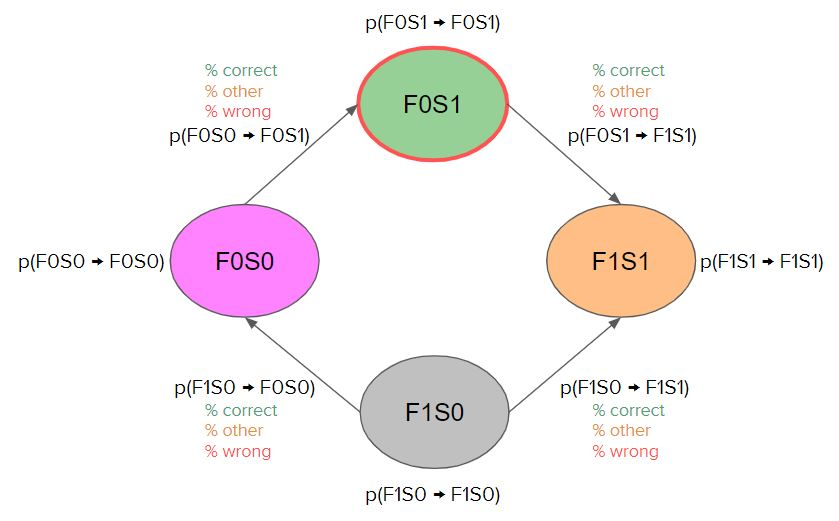
\includegraphics[width=.8\linewidth]{figures/fsm_example.jpg}
    \caption{ Example of a Finite State Machine }
    \label{fig:fsm_example}
\end{figure}
A few final notes on the FSM representation:
\begin{itemize}
    \item probabilities and percentages are extracted from the dev set
    \item self loop transitions are omitted from the graphical representation
    \item the sum of probababilities of outgoing transitions, including self loops, must be equal to 1
\end{itemize}

\subsubsection{Results on FIGER}
Only for these experiments, a reduced version of FIGER is used with the purpose to anticipate training convergence. The subset of the dataset is extracted by a random sample that counts approximately 267K training examples.
\paragraphn{Quantitative analysis 1 - Clause weights}
The performance in terms of \textit{macro f1 examples} obtained by varying the initial clause weights is available in Figure~\ref{fig:wandb_weights_comparison}. Looking at the graphs, we can observe a common behavior: regardless of the KB mode, the influence of different weights is visible only in the first 15-20 epochs (i.e., the red line in the graph is above the others in the initial epochs). Especially for the Hybrid mode, we can see in Figure~\ref{fig:wandb_weights_comparison_h} how the largest weight gives a clear initial boost to the performance. However, the boost tends to diminish over the epochs until it disappears. Another interesting behavior can be found in Figure~\ref{fig:wandb_weights_avg_pred_start}, which shows the evolution of the \textit{average predictions number} in the first 20 epochs. From the figures, we can observe that the larger the weight, the higher the number of predictions, and the larger the weight, the higher the performance. We can deduce from these results that the increased performance is due to an increased number of correct predictions, otherwise we would not see an increment in the performance. To conclude, we can say that a major influence of KENN helps the network to learn faster when it has not yet seen a big amount of training examples.
\\\\
\textit{\textbf{Note:} the previous considerations still apply to the other metrics not reported here}

\begin{figure}
     \centering
     \begin{subfigure}{0.8\textwidth}
         \centering
         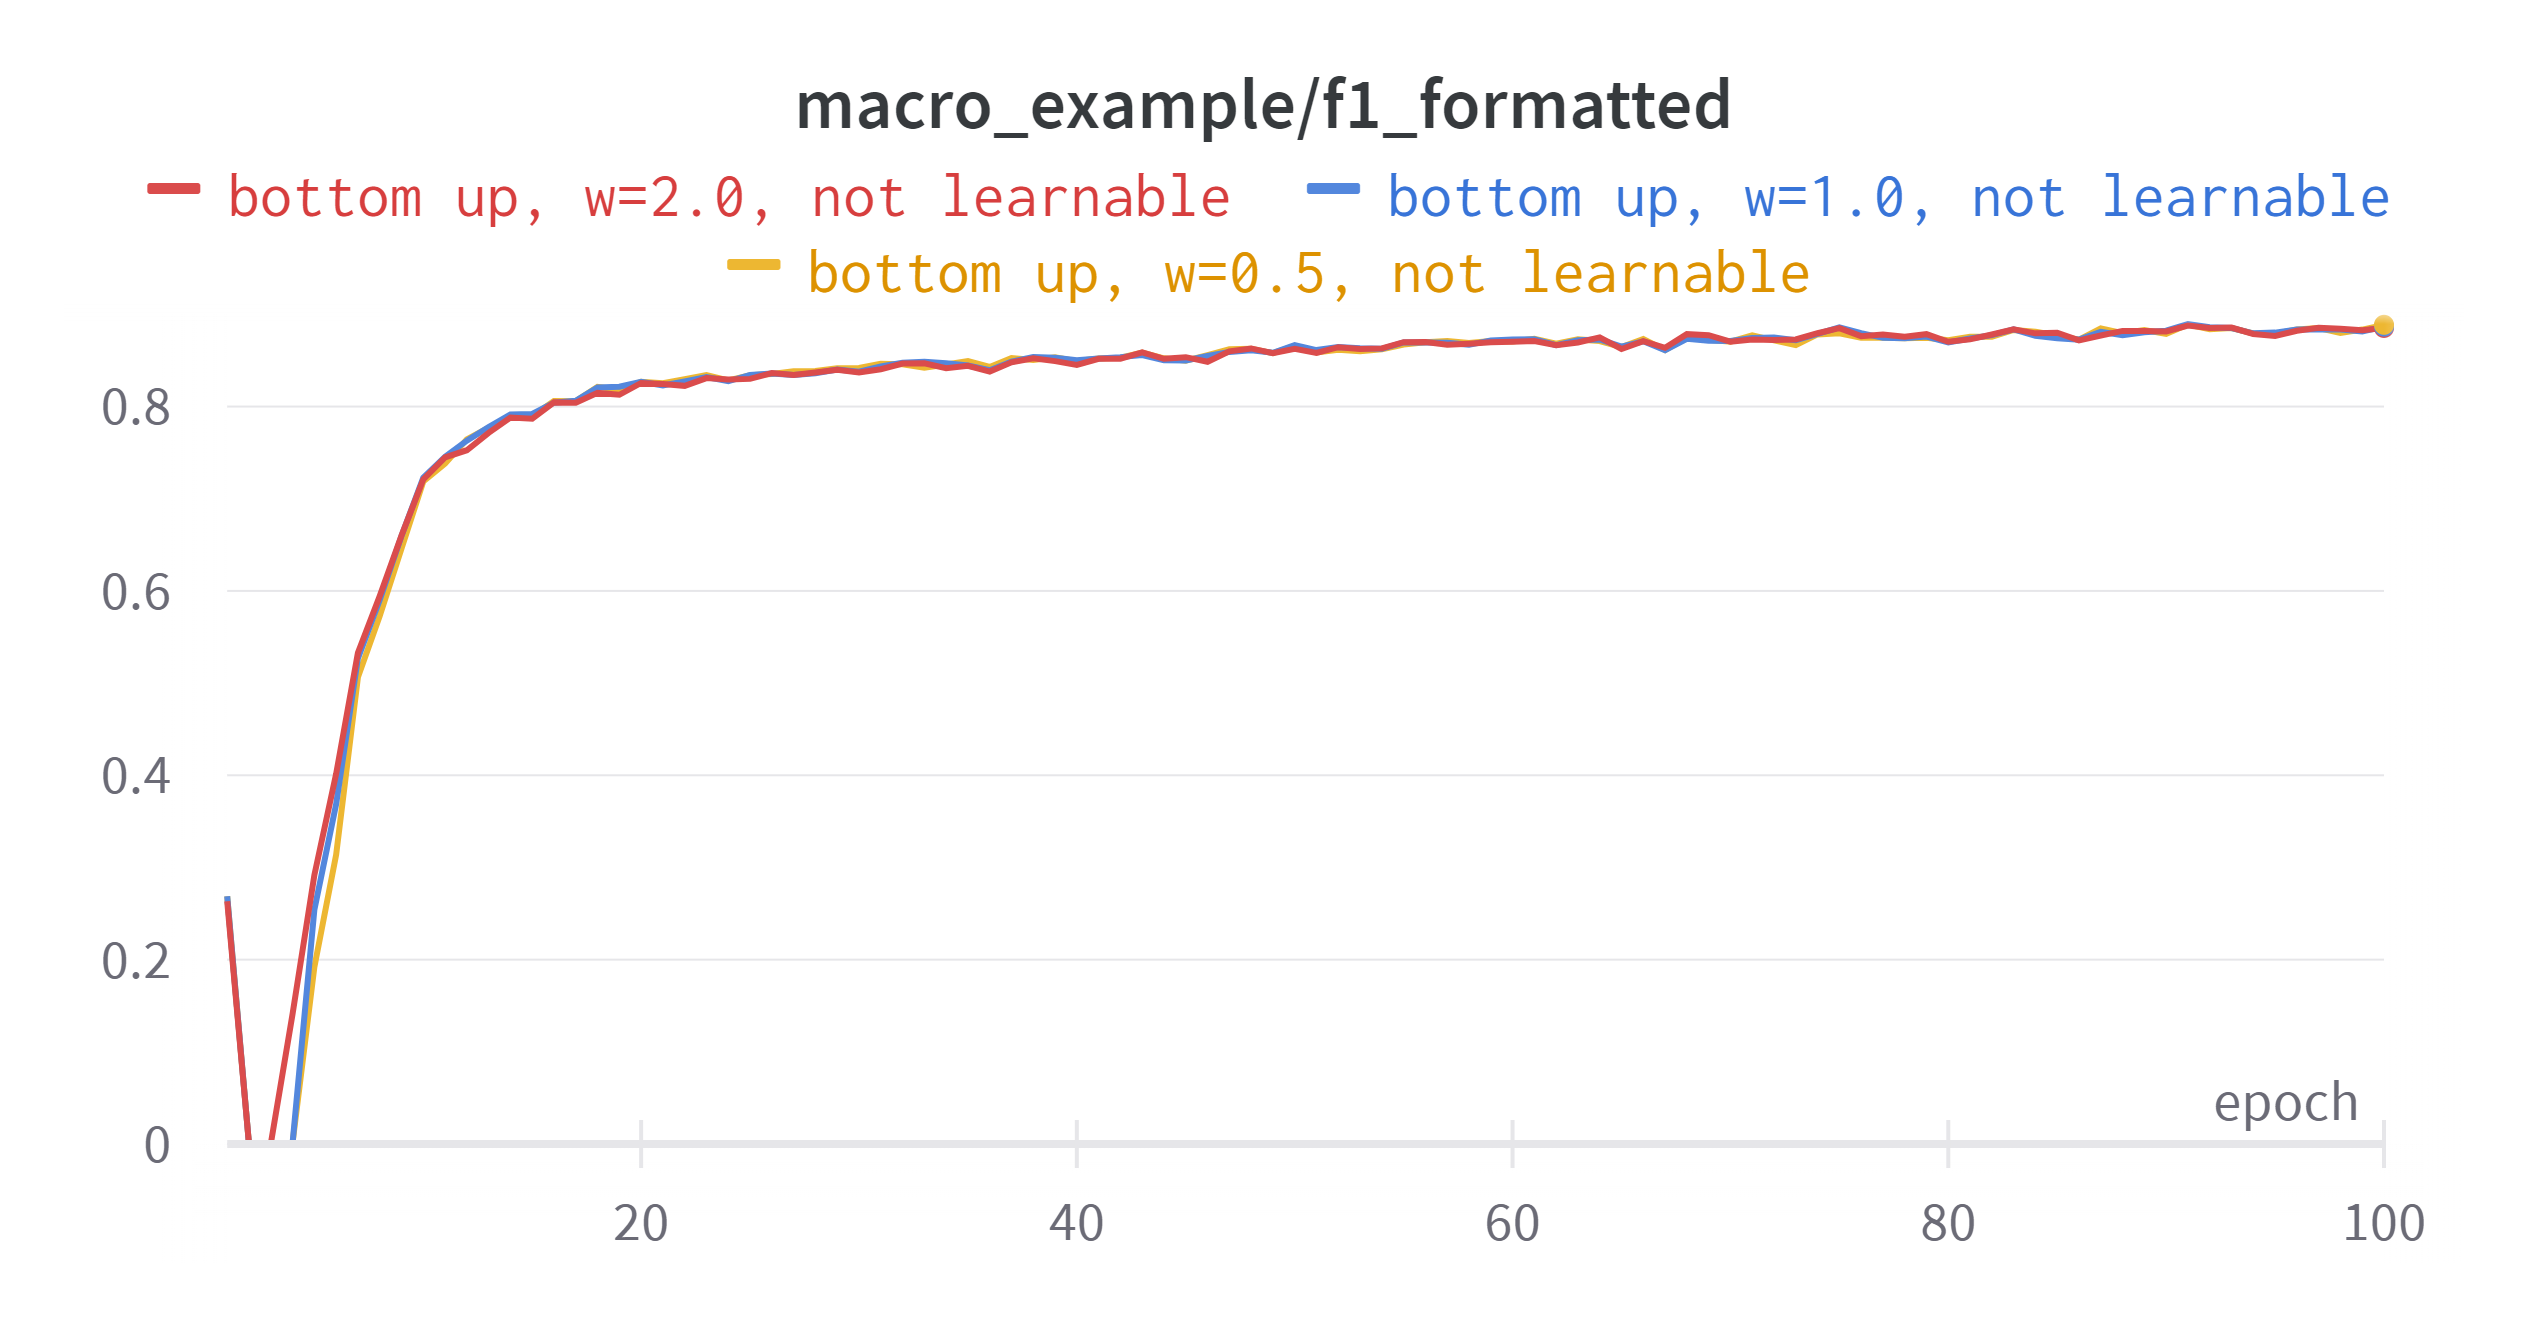
\includegraphics[width=\textwidth]{figures/wandb_weights_bottom_up_macro_ex_f1.png}
         \caption{Bottom Up}
     \end{subfigure}
     \vfill
     \begin{subfigure}{0.8\textwidth}
         \centering
         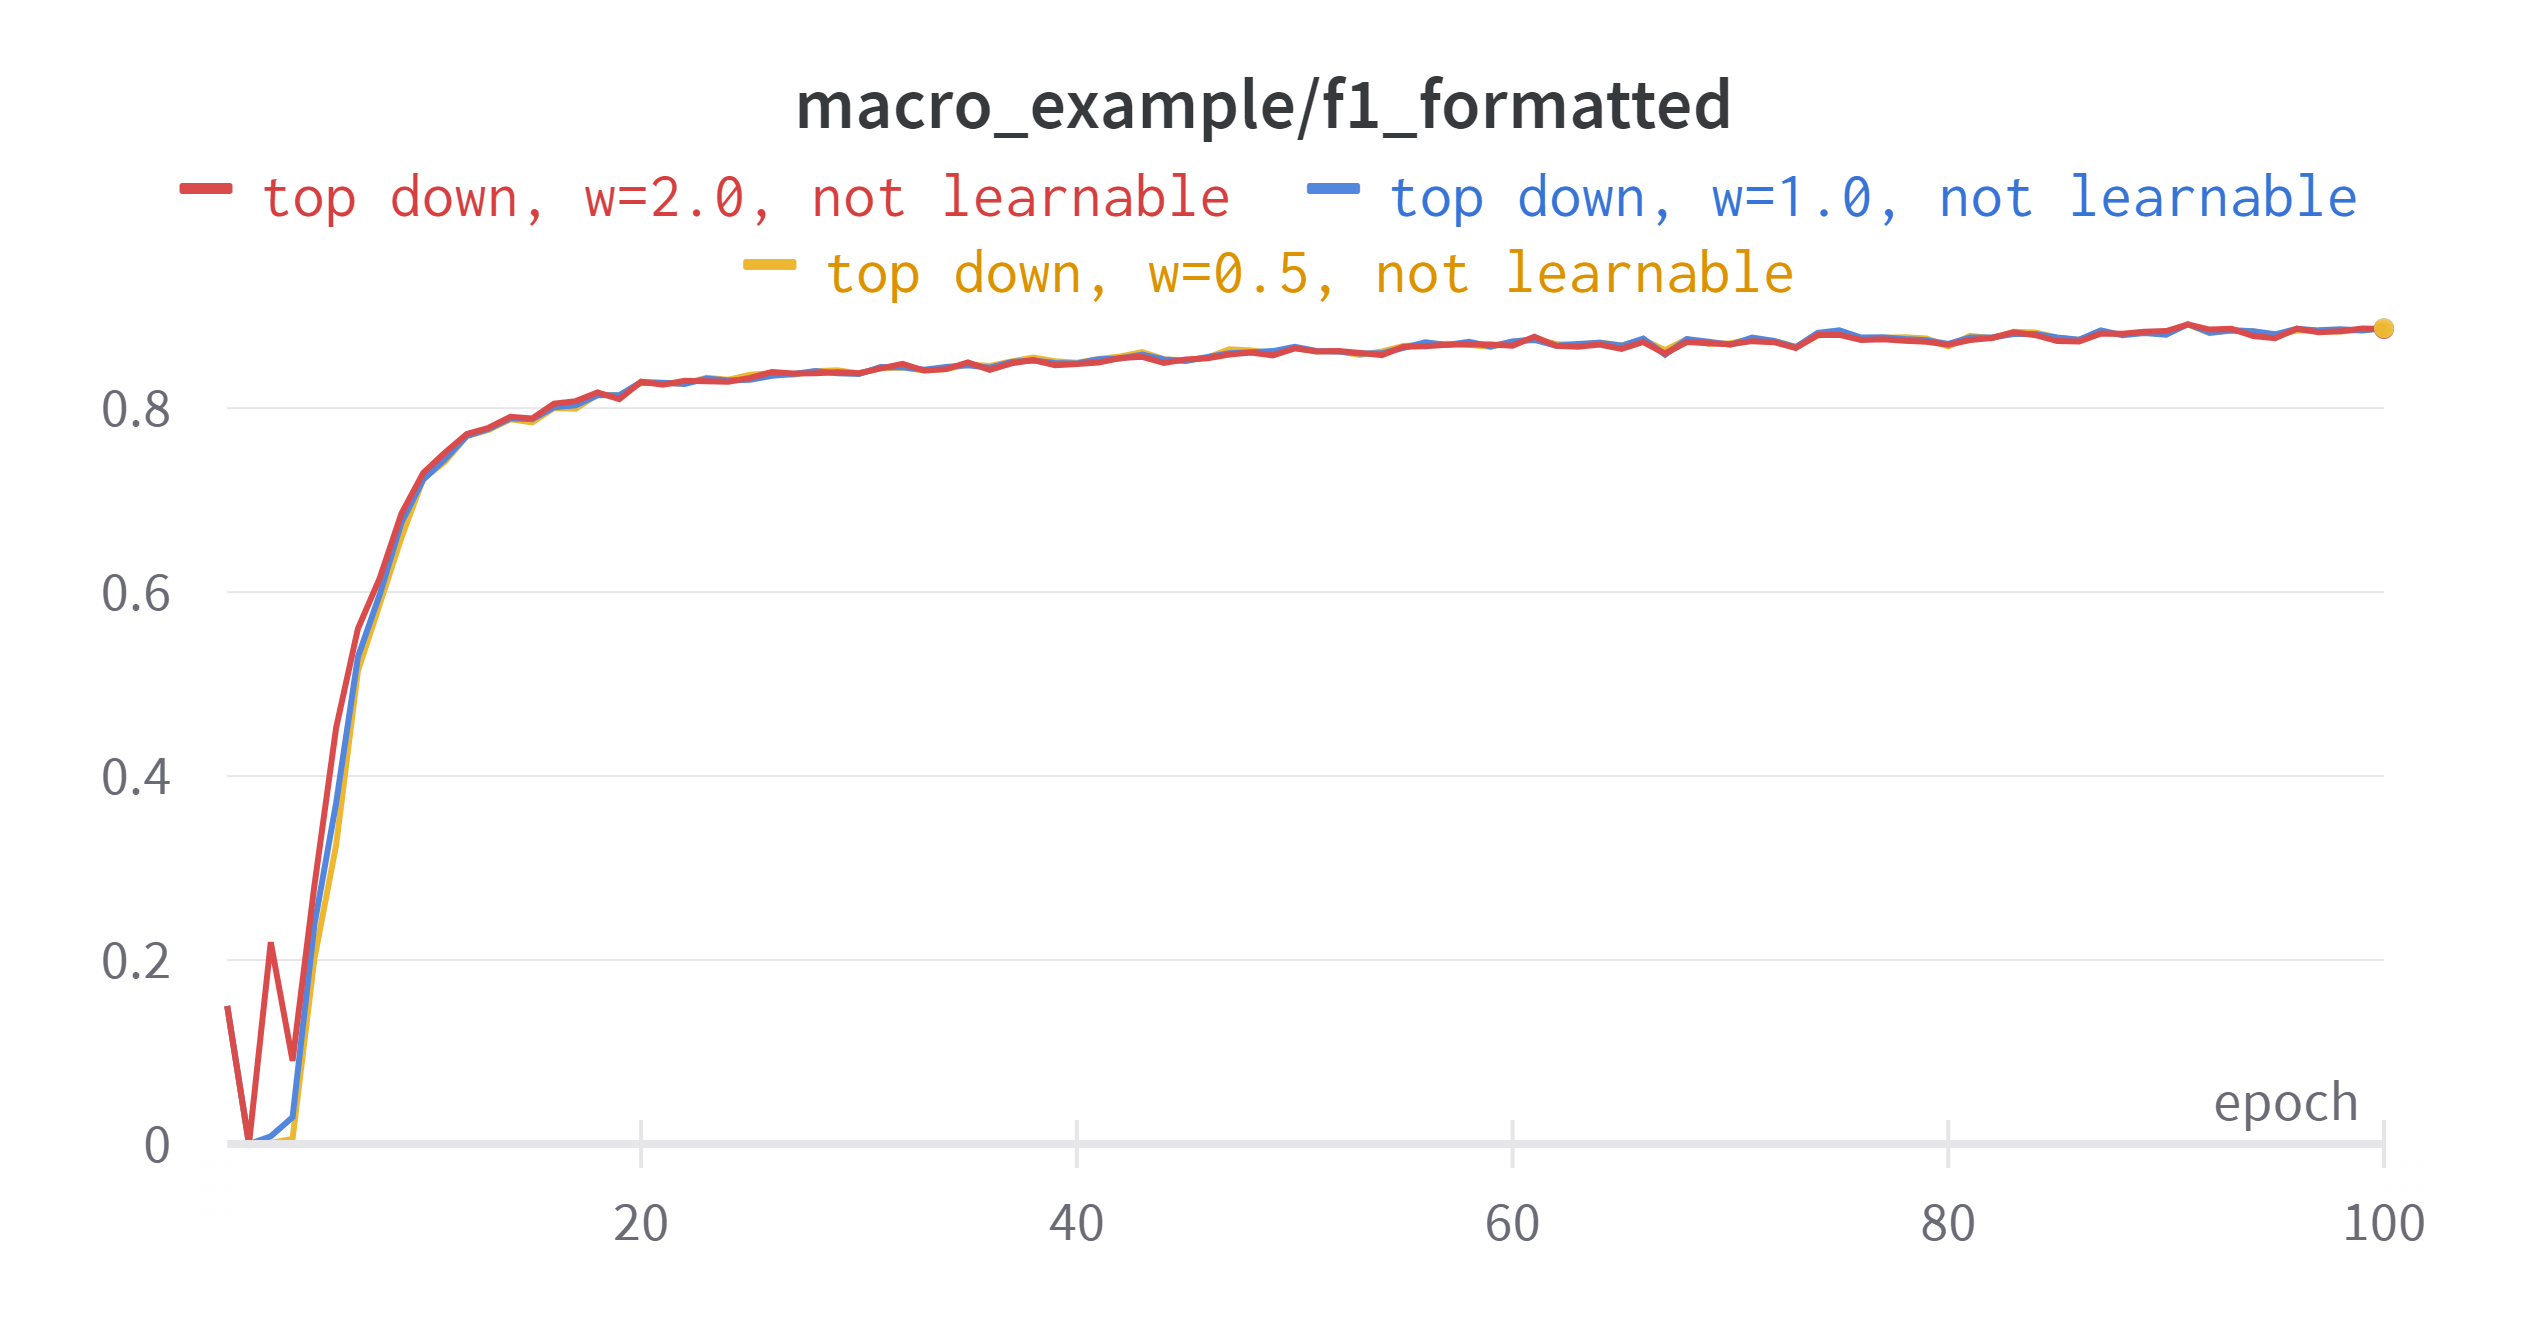
\includegraphics[width=\textwidth]{figures/wandb_weights_top_down_macro_ex_f1.png}
         \caption{Top Down}
     \end{subfigure}
     \vfill
     \begin{subfigure}{0.8\textwidth}
         \centering
         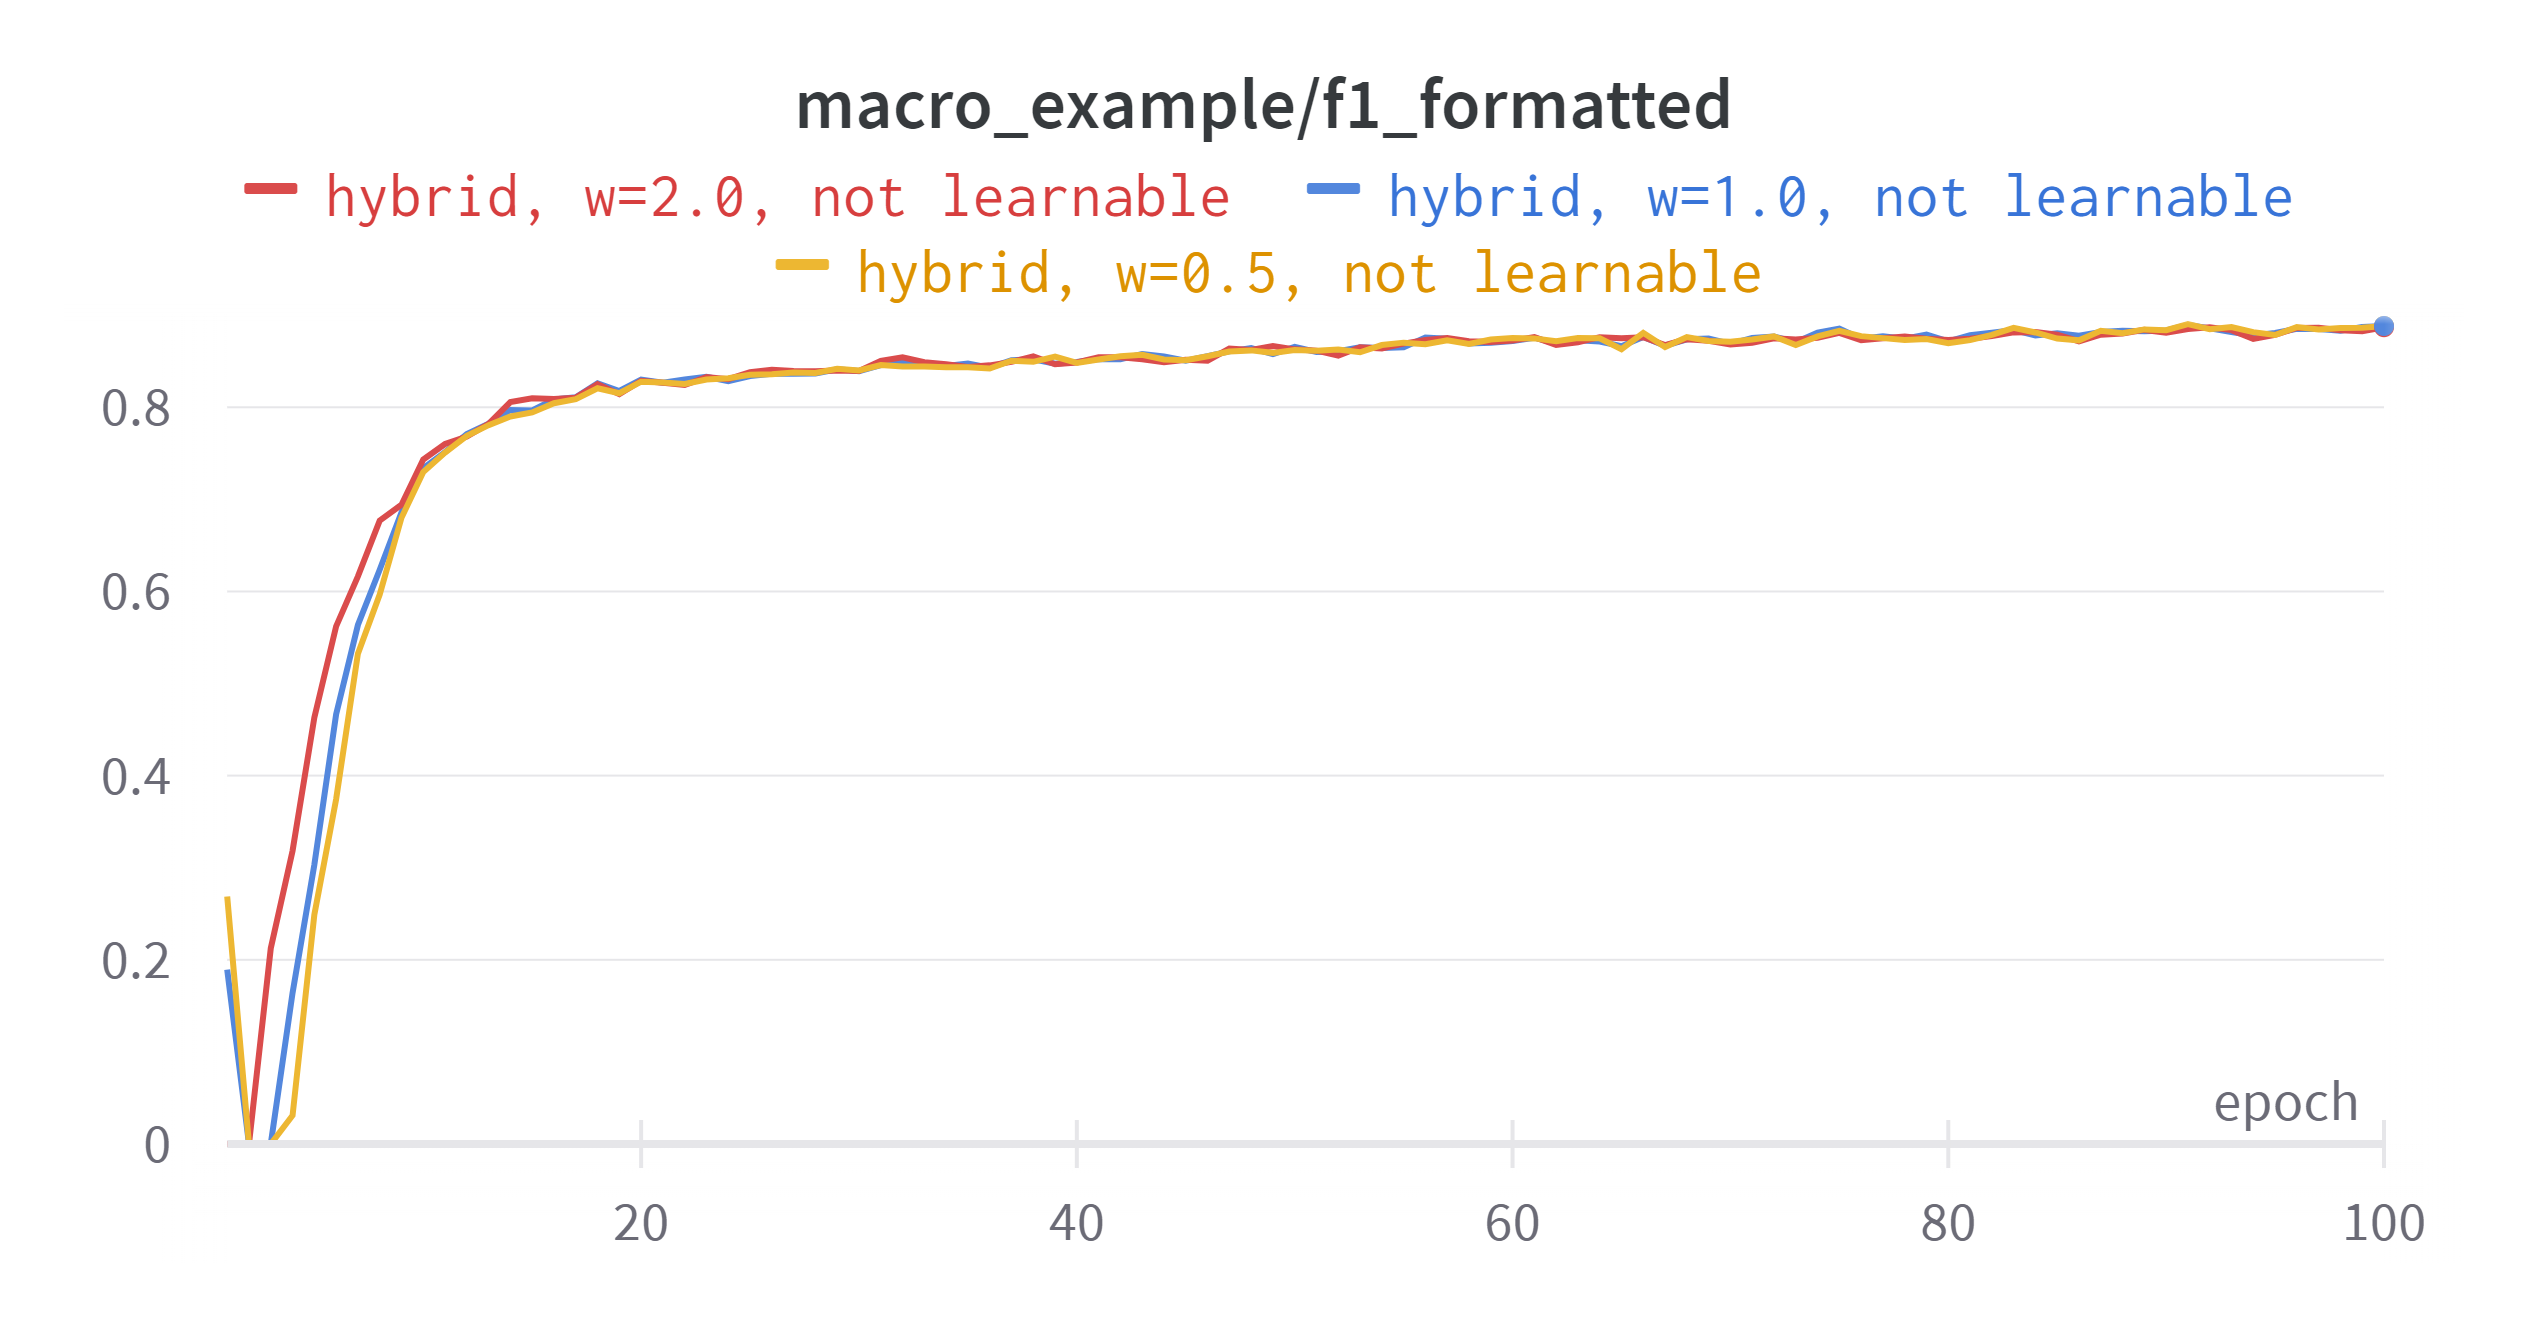
\includegraphics[width=\textwidth]{figures/wandb_weights_hybrid_macro_ex_f1.png}
         \caption{Hybrid}
         \label{fig:wandb_weights_comparison_h}
    \end{subfigure}
        \caption{Comparison of \textit{macro f1 examples} by varying the clause weight for each KB mode, with DistilBERT-based models evaluated on the dev set of FIGER.}
        \label{fig:wandb_weights_comparison}
\end{figure}

\begin{figure}
     \centering
     \begin{subfigure}{0.8\textwidth}
         \centering
         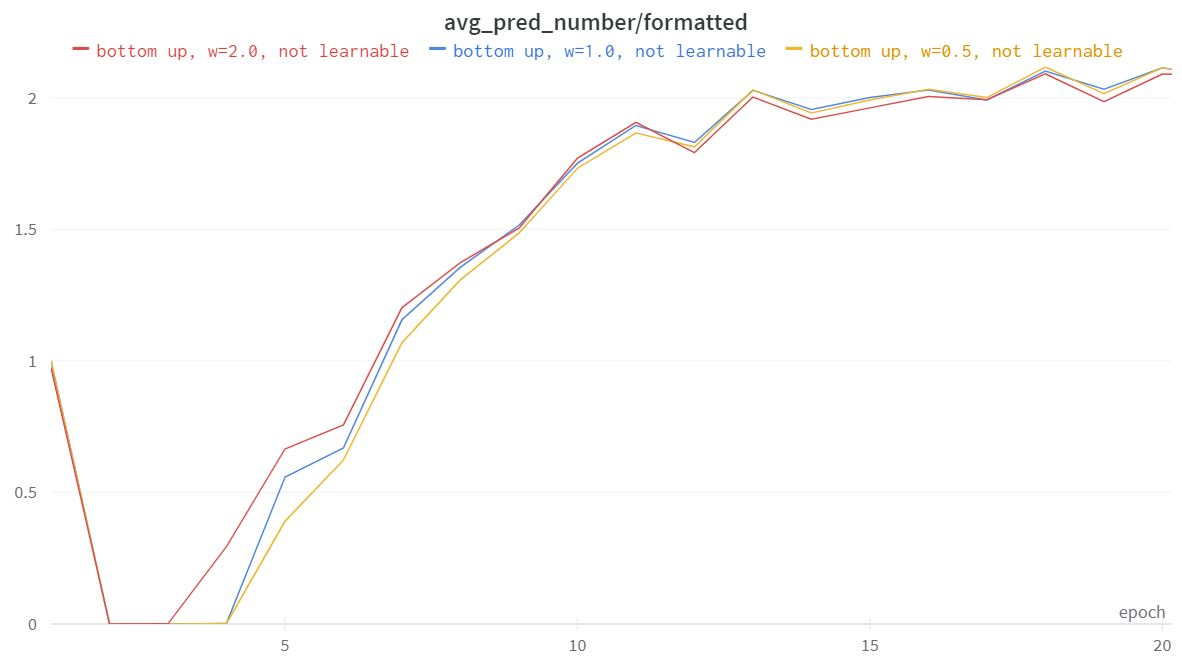
\includegraphics[width=\textwidth]{figures/wandb_weights_bottom_up_avg_pred_start.JPG}
         \caption{Bottom Up}
     \end{subfigure}
     \vfill
     \begin{subfigure}{0.8\textwidth}
         \centering
         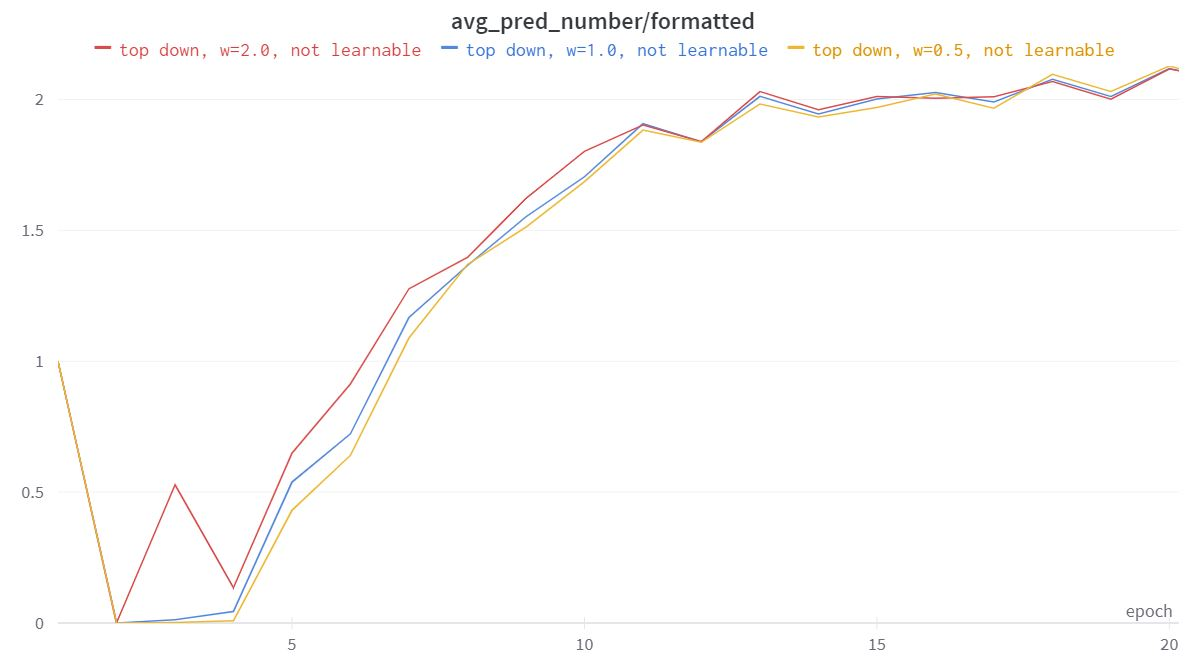
\includegraphics[width=\textwidth]{figures/wandb_weights_top_down_avg_pred_start.JPG}
         \caption{Top Down}
     \end{subfigure}
     \vfill
     \begin{subfigure}{0.8\textwidth}
         \centering
         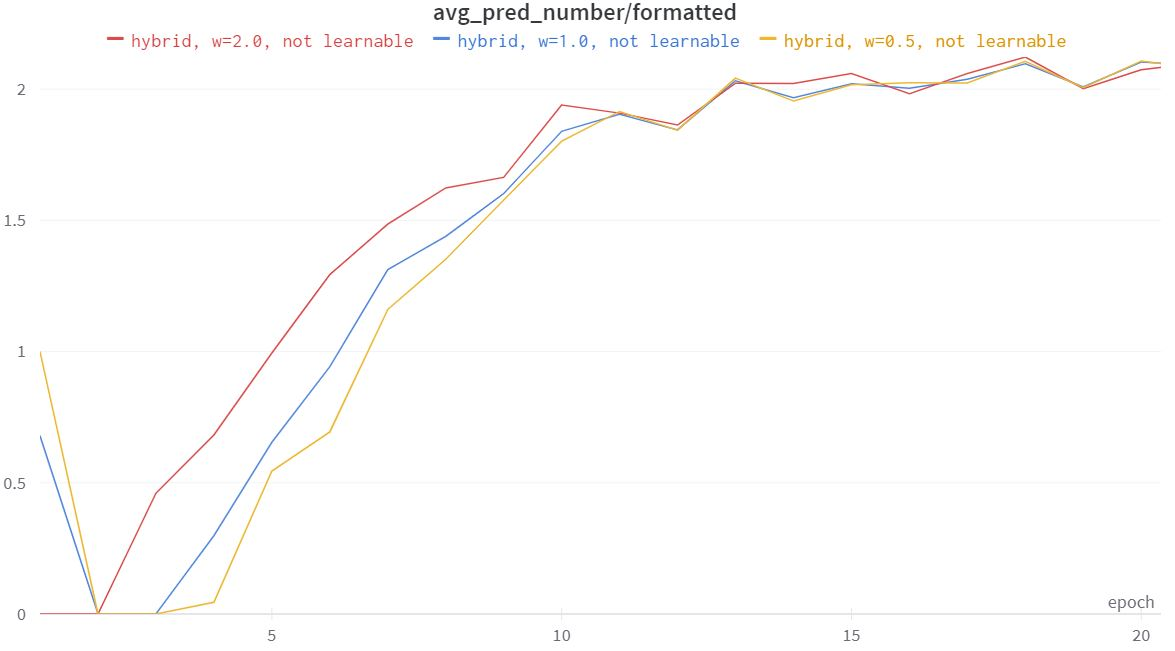
\includegraphics[width=\textwidth]{figures/wandb_weights_hybrid_avg_pred_start.JPG}
         \caption{Hybrid}
     \end{subfigure}
        \caption{Comparison of \textit{average predictions number} by varying the clause weight for each KB mode, with DistilBERT-based models evaluated on the dev set of FIGER. Zoom on the first 20 epochs.}
        \label{fig:wandb_weights_avg_pred_start}
\end{figure}

\paragraphn{Quantitative analysis 2 - KB modes}
Moving on to the comparison between the KB modes, 3 model instances per configuration were trained by varying the random seed. The initial clause weight is set to 2.0 because in the previous experiment was the one that obtained the biggest boost. Figure~\ref{fig:wandb_modes_comparison} reports the comparison graphs in terms of \textit{average predictions number}, \textit{macro f1 examples} and \textit{macro f1 classes }. Similarly to the comparison of the weight, we can draw some considerations about the first steps of the training. Starting from the \textit{average predictions number}, we can clearly observe that the baseline model (i.e, \textit{kb\_mode: - }) produces significantly fewer predictions than KENN in the early stage. In particular, we can notice that the baseline is not able to produce any prediction for the first 4 epochs. Since the pre-KENN network and the baseline network have the same initialization, the fact that KENN requires fewer epochs to make correct predictions is due to the use of logical knowledge.

\begin{figure}[h]
    \centering
    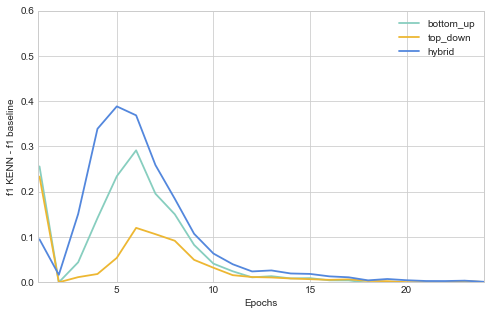
\includegraphics[scale=0.4]{figures/initial_boost.png}
    \caption{Difference between the \textit{macro f1 examples} scores of KENN and baseline models with DistilBERT encoder, evaluated on the dev set of FIGER. The curves are averaged over 3 random seeds. Zoom on the first 25 epochs.}
    \label{fig:initial_boost}
\end{figure}

The trend observed in the \textit{average predictions number} is also detectable by all the other metrics. Figure~\ref{fig:initial_boost} highlights the initial boost of KENN-based models by measuring the difference with respect to the baseline in terms of \textit{macro f1 examples}. The behavior that consolidates as the seeds vary is that Hybrid starts better than Bottom Up, which starts better than Top Down. The baseline model, instead, is the one with the slowest start. The cause of this initial ranking may be that the Hybrid mode can exploit the logical rules of both Bottom Up and Top Down modes. In the second part of the training, instead, the models converge to each other and keep improving together. The results of the final models are reported in Table~\ref{tab:kb_modes_comparison} and are very similar for each KB mode.
% Looking at the graphs in their entirety, there is not a dominant model. However, by looking at the \textit{macro f1 classes} graph we can observe that the baseline model is the only one which never takes the lead.
\begin{figure}
     \centering
     \begin{subfigure}{0.8\textwidth}
         \centering
         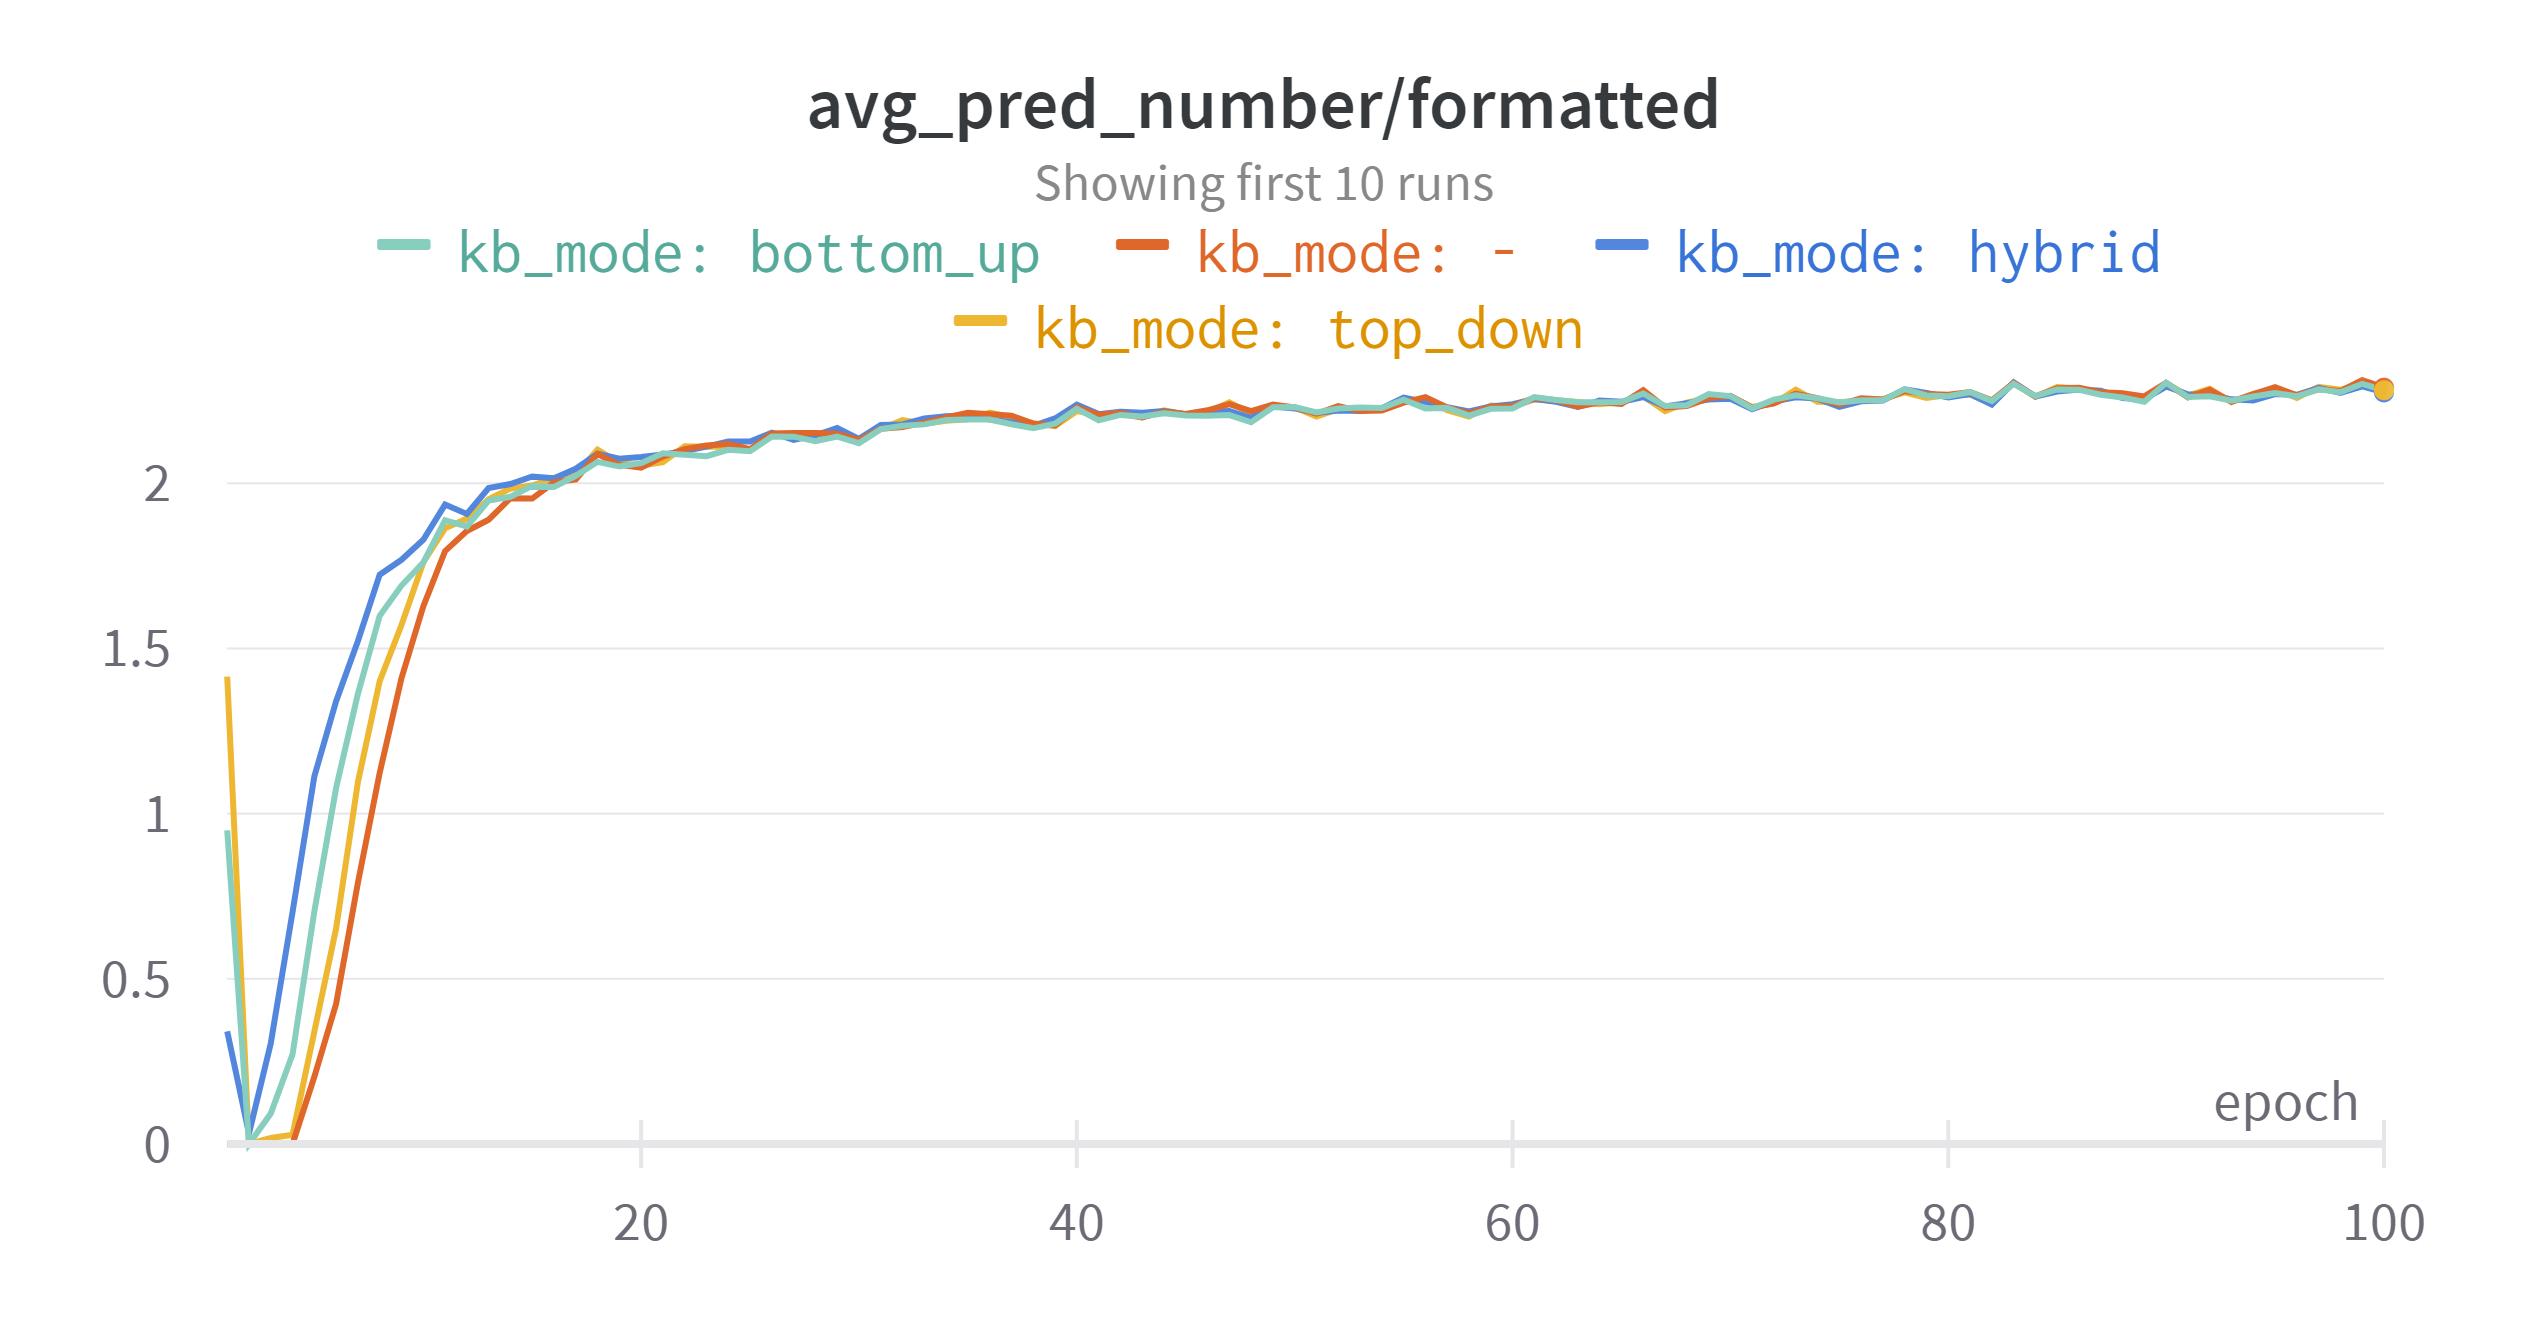
\includegraphics[width=\textwidth]{figures/wandb_modes_avg_pred.png}
         \caption{Average predictions number}
     \end{subfigure}
     \begin{subfigure}{0.8\textwidth}
         \centering
         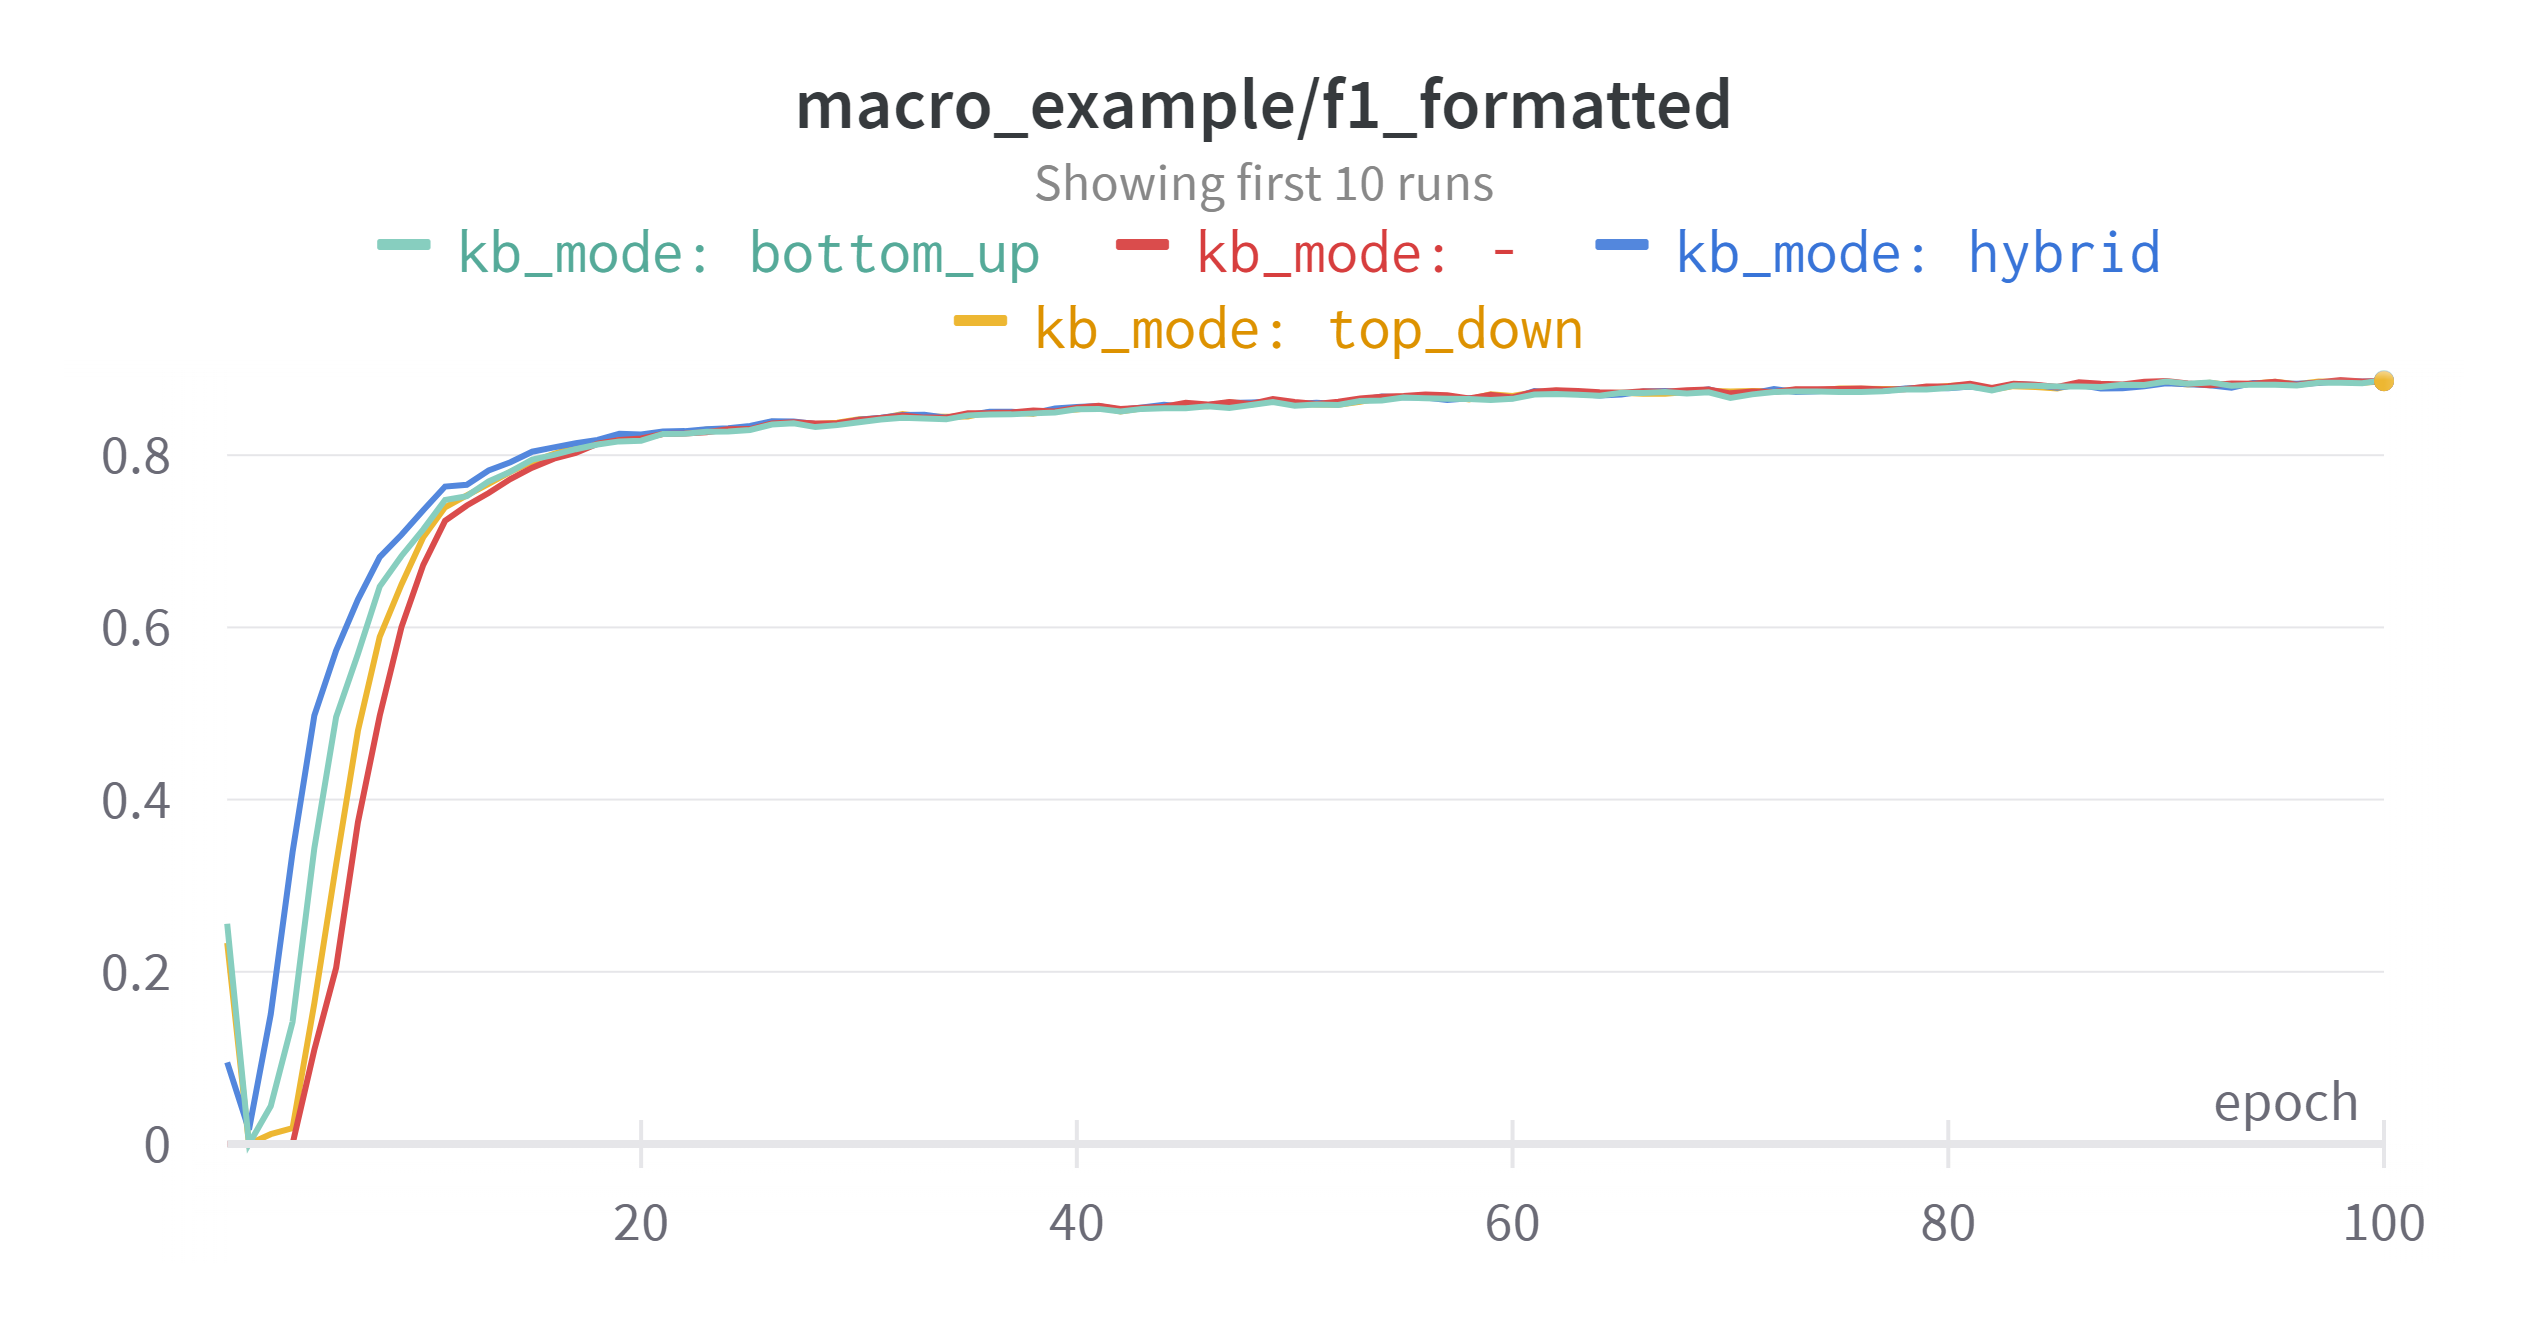
\includegraphics[width=\textwidth]{figures/wandb_modes_macro_ex_f1.png}
         \caption{Macro f1 examples}
     \end{subfigure}
     \begin{subfigure}{0.8\textwidth}
         \centering
         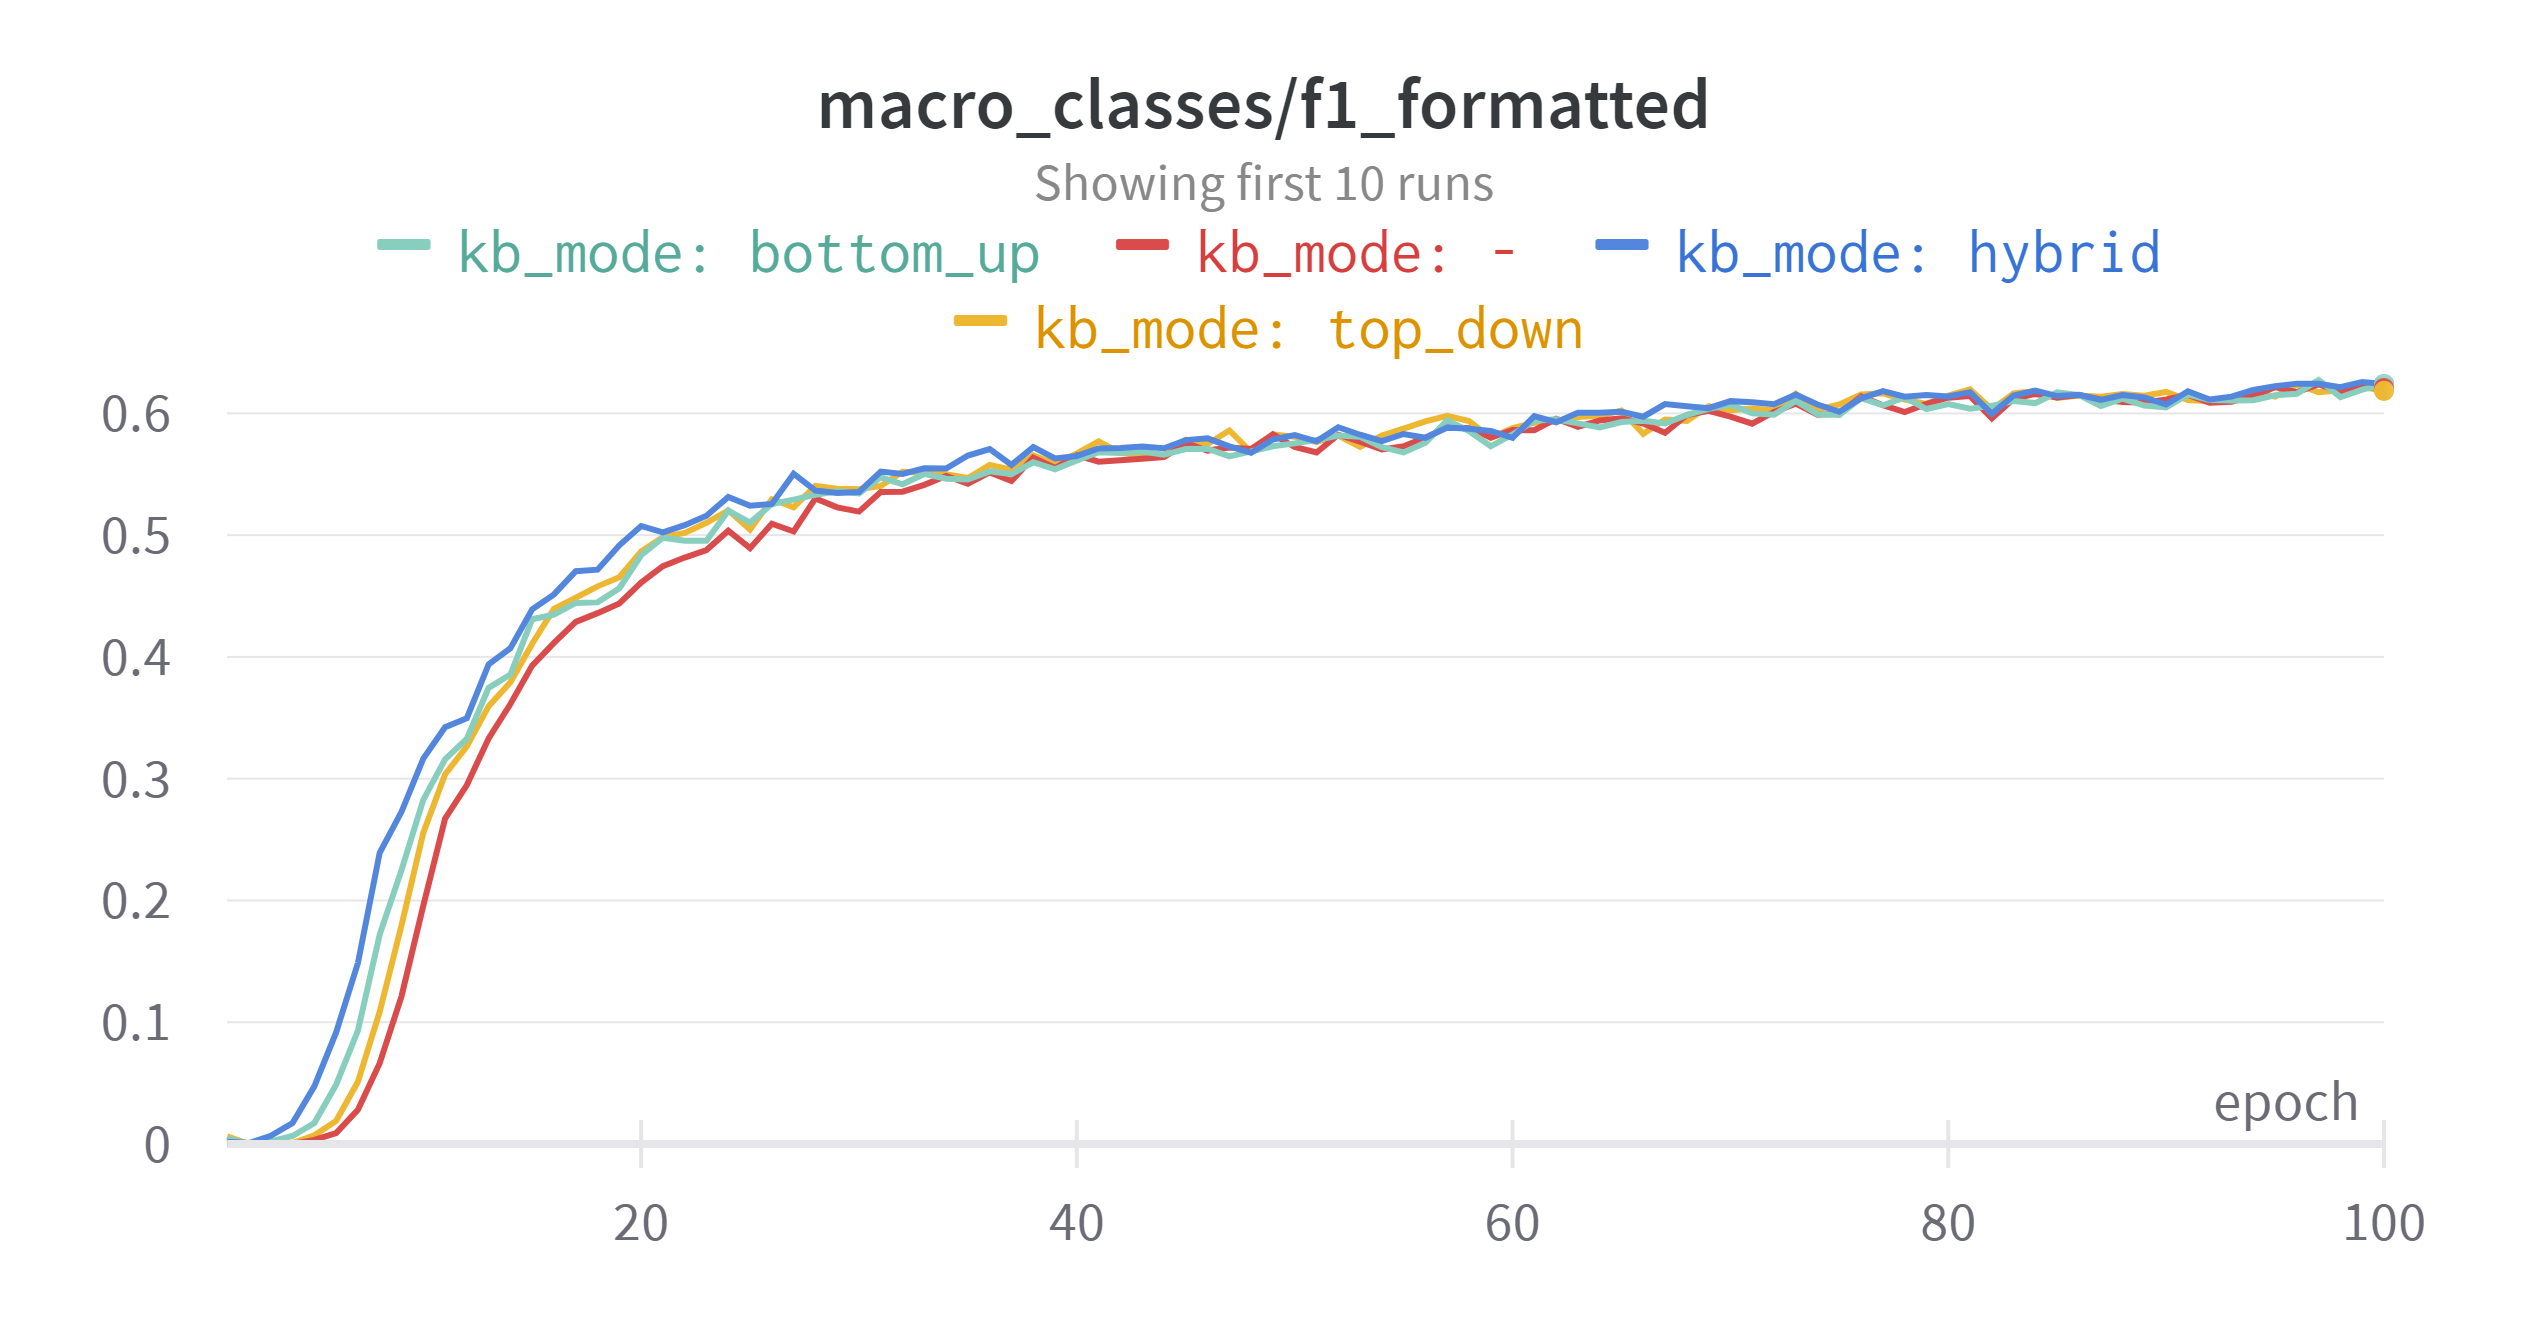
\includegraphics[width=\textwidth]{figures/wandb_modes_macro_class_f1.png}
         \caption{Macro f1 classes}
     \end{subfigure}
        \caption{Comparison between KENN with clause weights fixed to 2.0 and baseline model with DistilBERT encoder, evaluated on the dev set of FIGER. Zoom on the first 20 epochs.}
        \label{fig:wandb_modes_comparison}
\end{figure}

\begin{table}
\centering
\caption{Comparison between KENN with clause weights fixed to 2.0 and baseline model evaluated on the dev set of FIGER. Metrics at epoch 100 averaged over 3 seeds.}
\label{tab:kb_modes_comparison}
\resizebox{\columnwidth}{!}{\begin{tabular}{c|ccc|ccc|}
\cline{2-7}
\textbf{}                            & \multicolumn{3}{c|}{\textbf{Macro examples}}                                                                                                                                                                             & \multicolumn{3}{c|}{\textbf{Macro classes}}                                                                                                                                                                              \\ \hline
\multicolumn{1}{|c|}{\textbf{KB mode}} & \textbf{P}                                                             & \textbf{R}                                                             & \textbf{F1}                                                            & \textbf{P}                                                             & \textbf{R}                                                             & \textbf{F1}                                                            \\ \hline
\multicolumn{1}{|c|}{- (baseline)}       & \begin{tabular}[c]{@{}c@{}}0.8944\\ $\pm$ 0.0009\end{tabular}          & \begin{tabular}[c]{@{}c@{}}0.8779\\ $\pm$ 0.0033\end{tabular}          & \begin{tabular}[c]{@{}c@{}}0.8861\\ $\pm$ 0.0021\end{tabular}          & \begin{tabular}[c]{@{}c@{}}0.6499\\ $\pm$ 0.0152\end{tabular}          & \begin{tabular}[c]{@{}c@{}}0.5943\\ $\pm$ 0.0051\end{tabular}          & \begin{tabular}[c]{@{}c@{}}0.6208\\ $\pm$ 0.0091\end{tabular}          \\ \hline
\multicolumn{1}{|c|}{Bottom Up}      & \begin{tabular}[c]{@{}c@{}}0.8963\\ $\pm$ 0.0.0020\end{tabular}        & \textbf{\begin{tabular}[c]{@{}c@{}}0.8783\\ $\pm$ 0.0047\end{tabular}} & \textbf{\begin{tabular}[c]{@{}c@{}}0.8872\\ $\pm$ 0.0020\end{tabular}} & \begin{tabular}[c]{@{}c@{}}0.6516\\ $\pm$ 0.0165\end{tabular}          & \textbf{\begin{tabular}[c]{@{}c@{}}0.5986\\ $\pm$ 0.0110\end{tabular}} & \begin{tabular}[c]{@{}c@{}}0.6239\\ $\pm$ 0.0115\end{tabular}          \\ \hline
\multicolumn{1}{|c|}{Top Down}       & \begin{tabular}[c]{@{}c@{}}0.8944\\ $\pm$ 0.0008\end{tabular}          & \begin{tabular}[c]{@{}c@{}}0.8777\\ $\pm$ 0.0029\end{tabular}          & \begin{tabular}[c]{@{}c@{}}0.8860\\ $\pm$ 0.0013\end{tabular}          & \begin{tabular}[c]{@{}c@{}}0.6484\\ $\pm$ 0.0088\end{tabular}          & \begin{tabular}[c]{@{}c@{}}0.5913\\ $\pm$ 0.0112\end{tabular}          & \begin{tabular}[c]{@{}c@{}}0.6185\\ $\pm$ 0.0010\end{tabular}          \\ \hline
\multicolumn{1}{|c|}{Hybrid}         & \textbf{\begin{tabular}[c]{@{}c@{}}0.8965\\ $\pm$ 0.0028\end{tabular}} & \begin{tabular}[c]{@{}c@{}}0.8759\\ $\pm$ 0.0025\end{tabular}          & \begin{tabular}[c]{@{}c@{}}0.8861\\ $\pm$ 0.0017\end{tabular}          & \textbf{\begin{tabular}[c]{@{}c@{}}0.6533\\ $\pm$ 0.0185\end{tabular}} & \begin{tabular}[c]{@{}c@{}}0.5974\\ $\pm$ 0.0050\end{tabular}          & \textbf{\begin{tabular}[c]{@{}c@{}}0.6241\\ $\pm$ 0.0112\end{tabular}} \\ \hline
\end{tabular}}
\end{table}

\paragraphn{Quantitative analysis 3 - Metrics per type}
We can observe some interesting behaviors by computing the metrics grouped per types F and S. Focusing on epoch 4 (i.e., the last epoch before the baseline model starts making predictions), it emerges that KENN predicts only types F. This result makes sense since an F type should be easier to predict than an S type, which is more specific. More in detail, Bottom Up and Top Down modes can lead the model to make predictions exclusively on the type \texttt{/location}, reaching an f1 score of 0.595 and 0.441 respectively. The Hybrid model, which achieves an f1 score of 0.747 on \texttt{/location}, can also predict instances of type \texttt{/person} and \texttt{/organization}.

If we now focus on epoch 100, we can observe that Bottom Up performs better than Top Down on types F, with an f1 score of 0.661 and 0.646 respectively. Conversely, if we group the metrics per type S, we can observe that Top Down is better than Bottom Up, with an f1 score of 0.563 and 0.546 respectively. This behavior is consistent with the nature of the different clauses: Bottom Up propagates the information to F, Top Down to S.

\paragraphn{Quantitative analysis - Conclusion}
This analysis points out that the more relevant differences are observable only at the beginning of the training. The initial gap between different clause weights is bridged after 15-20 epochs, as does the difference between the KB modes. The same behavior can be observed when comparing KENN to the baseline model. The suspicion emerging from these considerations is that, at some point of the training, the baseline model becomes as powerful as the KENN-based models. 
%This suspicion can also be extended to the pre-KENN network, which increases its prediction capabilities epoch after epoch, needing less and less KENN's help.
From this premises we can sketch the following hypothesis: the pre-KENN network may adapt its output to obtain some desired predictions after the knowledge enhancement. This hypothesis will be further investigated with the analysis of the preactivations.
\paragraphn{Preactivations analysis 1 - Distributions}
We concluded the quantitative analysis leaving an open question: does the pre-KENN network adapt its predictions to KENN's action? To answer this question, we can start by examining the distribution of the preactivations of every final model. Each distribution will be split into two graphs to simplify the comparison by separating positive and negative predictions using different scales. Figure~\ref{fig:baseline_distrib} shows the distributions of the baseline model that will be used as a reference point. The values of $x$ are the preactivations of each type of each example, while the $y$ represents the frequency of a bin of preactivations.

We will start by comparing the positive predictions. In Figure~\ref{fig:kenn_pos_distrib} we can find the positive distributions of the KENN-based models. The first thing we can observe is that each KB mode produces very different pre-KENN distributions. If we look at the means (Bottom Up: 2.706, Top Down: 3.633, Hybrid: 2.227) and standard deviations (Bottom Up: 1.737, Top Down: 2.190, Hybrid: 1.434), we can also assert that they differ a lot from the baseline positive distribution (mean: 4.246, standard deviation: 2.228). On the contrary, the situation is completely different when looking at the post-KENN preactivations, since the intervention of KENN makes the distributions more similar to each other (means: 4.100$\pm$0.043, standard deviations: 2.058$\pm$0.038) and to the baseline. The same phenomenon can be observed by comparing the negative distribution of the baseline in Figure~\ref{fig:baseline_neg_distrib} to the pre-KENN and post-KENN negative distributions in Figure~\ref{fig:kenn_neg_distrib}.

\begin{figure}[H]
     \centering
     \begin{subfigure}{0.5\textwidth}
         \centering
         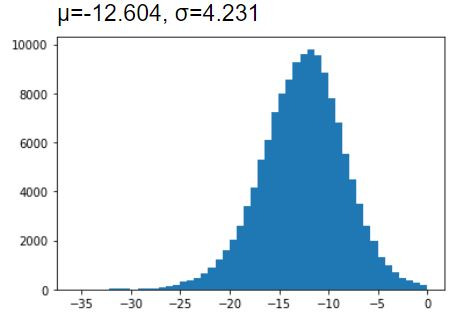
\includegraphics[width=\textwidth]{figures/baseline_neg.JPG}
         \caption{Negative preactivations}
         \label{fig:baseline_neg_distrib}
     \end{subfigure}
     \hfill
     \begin{subfigure}{0.475\textwidth}
         \centering
         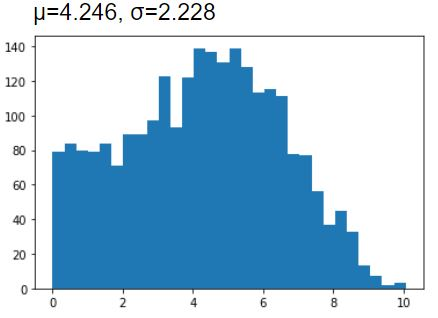
\includegraphics[width=\textwidth]{figures/baseline_pos.JPG}
         \caption{Positive preactivations}
         \label{fig:baseline_pos_distrib}
     \end{subfigure}
        \caption{Distribution of the baseline preactivations computed on the dev set of FIGER}
        \label{fig:baseline_distrib}
\end{figure}


\begin{figure}[H]
    \centering
    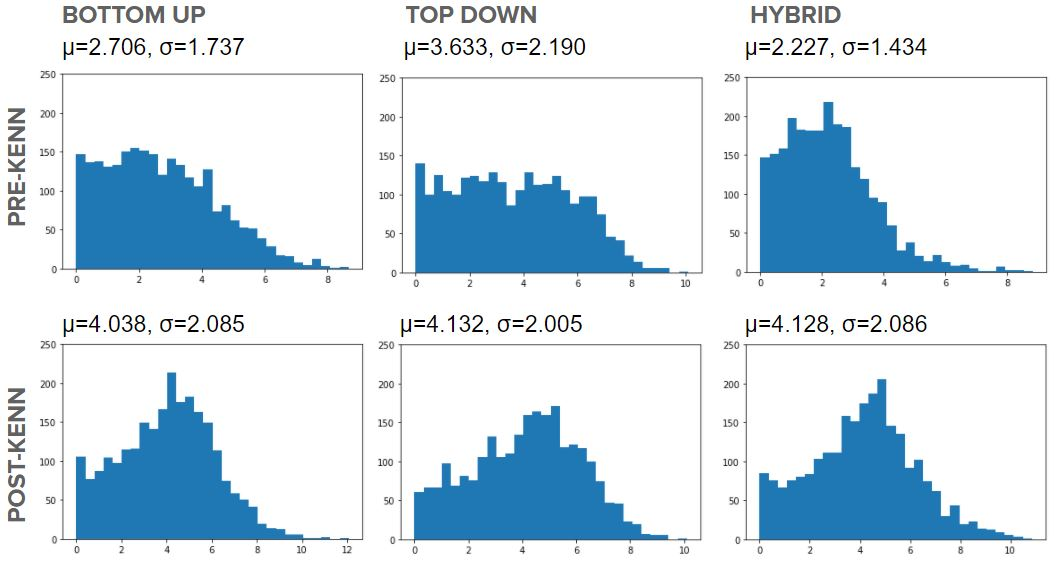
\includegraphics[scale=.53]{figures/kenn_pos_distrib.JPG}
    \caption{Distribution of the pre-KENN and post-KENN positive preactivations for each KB mode. Computed on the dev set of FIGER.}
    \label{fig:kenn_pos_distrib}
\end{figure}

\begin{figure}[H]
    \centering
    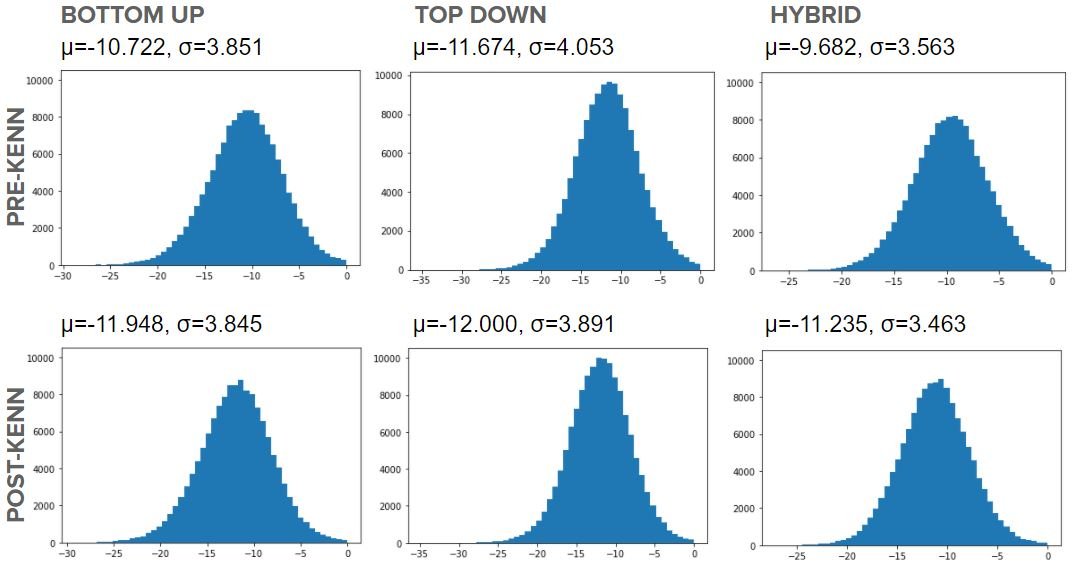
\includegraphics[scale=.53]{figures/kenn_neg_distrib.JPG}
    \caption{Distribution of the pre-KENN and post-KENN negative preactivations for each KB mode. Computed on the dev set of FIGER.}
    \label{fig:kenn_neg_distrib}
\end{figure}

\paragraphn{Preactivations analysis 2 and 3 - FSM and Sankey diagrams}
The analysis of the Finite State Machines and the Sankey diagrams can help to understand how the pre-KENN and post-KENN preactivations are modified depending on types F and S involved in the same clause, thus providing other insights into the suspicion of adaptation emerged in the previous study.

Starting from the Bottom Up mode, we can find the FSM and the Sankey diagram in Figure~\ref{fig:transitions_bottom_up}. We remind that a Bottom Up clause will always produce a positive delta on F and a negative delta on S. Indeed, F1S0 is a sink vertex of the Bottom Up FSM because F can never be decreased and S can never be increased in a Bottom Up setup. By analyzing the information of the transitions, we can observe that:
\begin{enumerate}
    \item The percentages of wrong transitions represent a minority.
    \item The probability of remaining in the forbidden state (i.e., F0S1) is 0.03. This is reasonable because the forbidden state represents also a clause violation (i.e., 1$\to$0) for this KB mode, so KENN will always try to modify the predictions to reach another post-KENN state. In these cases, the percentages of correctness show that the outgoing transitions from F0S1 never lead to worse predictions, but this is trivial since it is a wrong state by definition.
    \item The statistics about the transition F0S1$\to$F1S0 are quite counterintuitive since F and S are reversed correctly in 43.1\% of cases. The fact that the pre-KENN network predicts F as negative and S as positive when the target is the opposite is curious. It is plausible that the pre-KENN network learned that a type F usually receives one or more positive boosts, so it produces an initial negative prediction being aware that KENN will correct the final value. 
    \item The transition F0S0$\to$F1S0 could seem weird too. It has a probability of 0.01 and a percentage of correctness of 84.3\%. Some of these transitions are due to the fact that in the Bottom Up mode a type F is involved in multiple clauses, so the positive boost could derive from one or more siblings of S. However, after an investigation, it emerged that there are several examples of transitions F0S$_{1,...,n}$0$\to$F1S$_{1,...,n}$0 where F becomes positive thanks to the aggregated boost of its negative children. In particular, on a total of 500 F0S0$\to$F1S0 transitions, in 78 of them the effect of a single S was sufficient to enhance F. Even this behavior could be explained by the fact that the pre-KENN network learned that F is used to receive positive boosts.
\end{enumerate}


\begin{figure}
     \centering
     \begin{subfigure}{0.7\textwidth}
         \centering
         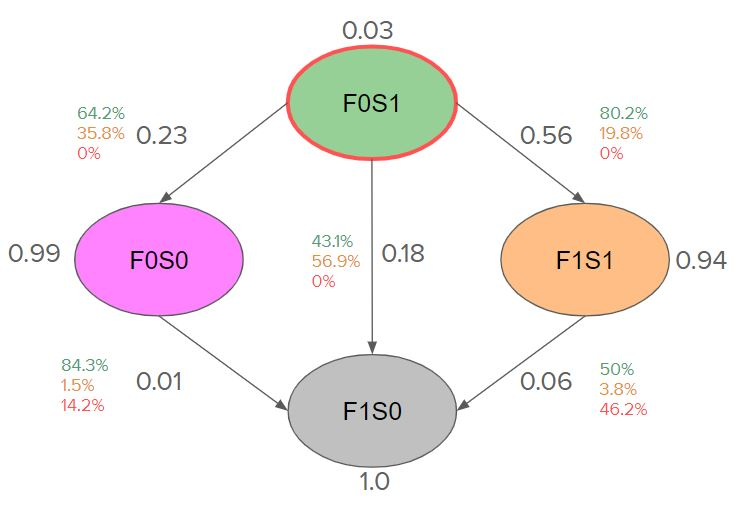
\includegraphics[width=\textwidth]{figures/fsm_bottom_up.JPG}
         \caption{FSM}
         \label{fig:fsm_bottom_up}
         \vspace{15px}
     \end{subfigure}
     \vfill
     \begin{subfigure}{0.6\textwidth}
         \centering
         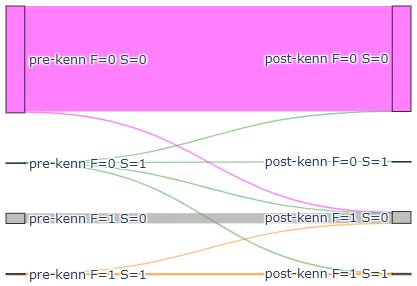
\includegraphics[width=\textwidth]{figures/sankey_bottom_up.JPG}
         \caption{Sankey diagram}
         \label{fig:sankey_bottom_up}
     \end{subfigure}
        \caption{FSM and Sankey diagram of the Bottom Up mode on the dev set of FIGER.}
        \label{fig:transitions_bottom_up}
\end{figure}

The FSM and the Sankey diagram of the Top Down mode are shown in Figure~\ref{fig:transitions_top_down}. The first thing we can notice is that the transitions of the FSM have opposite directions with respect to Bottom Up, so the sink vertex becomes F0S1. Looking at the statistics of the transitions, we can observe that:
\begin{enumerate}
    \item The percentages of wrong transitions represent a minority.
    \item The incoming transitions of the forbidden state have null probabilities when starting from F0S0 or F1S1, and near-zero probability when the pre-KENN state is F1S0. This is a very interesting fact, since it means that the pre-KENN network produces predictions such that KENN cannot generate a boost that leads to the forbidden state.
    \item Even if in this KB mode the pre-KENN state F1S0 may represent a clause violation (i.e., 1$\to 0 \vee ... \vee 0$) that KENN will try to correct, we can still find some examples of self-loop transition. Note that the high probability of 0.867 is due to the fact that in a Top Down clause the consequent is a disjunction of siblings. However, if we exclude from the count the cases in which a sibling of S is positive, we still have a high probability of 0.512 of self-loop. This means that the pre-KENN network learned to generate preactivations that prevent the effect of KENN when the desired output is F1S0.
    \item If we look at the Sankey diagram in Figure~\ref{fig:sankey_top_down}, we can see that the pre-KENN state F0S1 (i.e., the sink node) is missing. In this case too, the reason can be found in the fact that the pre-KENN network is aware that KENN will not be able to change the final predictions.
\end{enumerate}

\begin{figure}
     \centering
     \begin{subfigure}{0.7\textwidth}
         \centering
         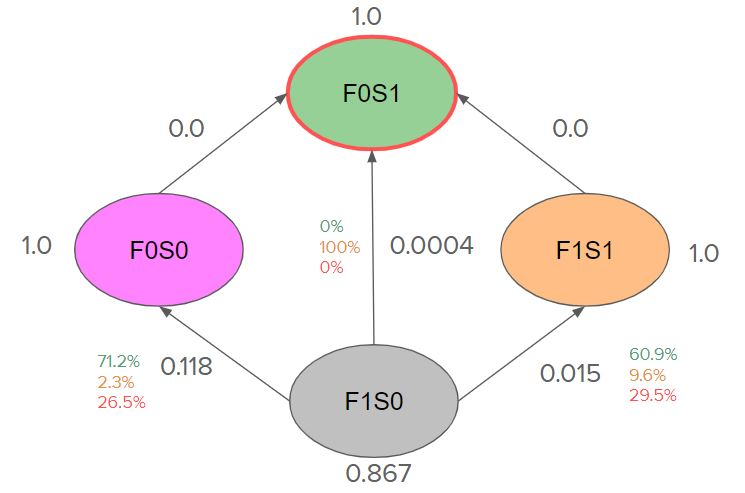
\includegraphics[width=\textwidth]{figures/fsm_top_down.JPG}
         \caption{FSM}
         \label{fig:fsm_top_down}
         \vspace{15px}
     \end{subfigure}
     \vfill
     \begin{subfigure}{0.6\textwidth}
         \centering
         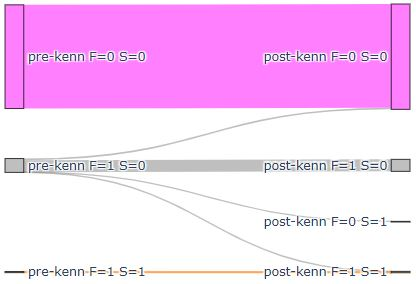
\includegraphics[width=\textwidth]{figures/sankey_top_down.JPG}
         \caption{Sankey diagram}
         \label{fig:sankey_top_down}
     \end{subfigure}
        \caption{FSM and Sankey diagram of the Top Down mode on the dev set of FIGER.}
        \label{fig:transitions_top_down}
\end{figure}

Finally, we can find the transitions of the Hybrid mode in Figure~\ref{fig:transitions_hybrid}. The FSM transitions are bidirectional because they are inherited from Top Down and Bottom Up. The consequence is that there are no sink nodes and all the transitions become potentially available. The considerations we can make by observing the figures are that:
\begin{enumerate}
    \item The percentages of wrong transitions represent a minority.
    \item Similarly to what happens in the Top Down, the probability to make a transition into the forbidden state is null.
    \item The probability of remaining in the forbidden state is very low like in the Bottom Up.
    \item The Sankey diagram is denser than those of Bottom Up and Top Down, since it is constituted by the mix of their transitions.
\end{enumerate}

\begin{figure}
     \centering
     \begin{subfigure}{0.7\textwidth}
         \centering
         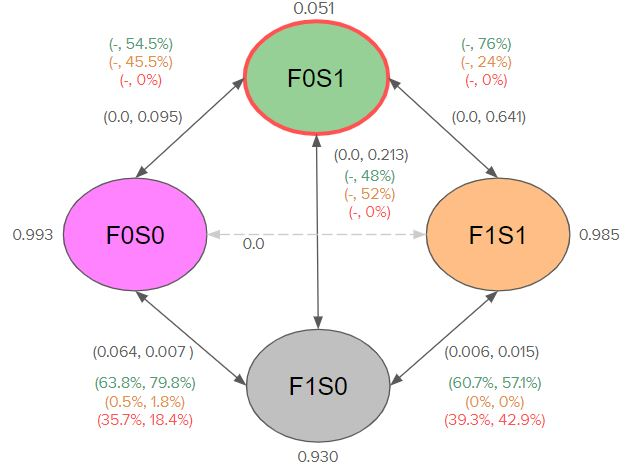
\includegraphics[width=\textwidth]{figures/fsm_hybrid.JPG}
         \caption{FSM - perecentages and probabilities are reported as \textit{(x, y)}, where \textit{x~=~value~of~down-to-up~transition} and \textit{y~=~value~of~up-to-down~transition}  }
         \label{fig:fsm_hybrid}
         \vspace{15px}
     \end{subfigure}
     \vfill
     \begin{subfigure}{0.6\textwidth}
         \centering
         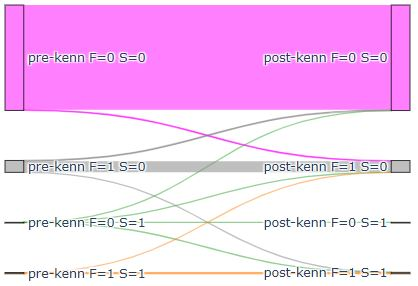
\includegraphics[width=\textwidth]{figures/sankey_hybrid.JPG}
         \caption{Sankey diagram}
         \label{fig:sankey_hybrid}
     \end{subfigure}
        \caption{FSM and Sankey diagram of the Hybrid mode on the dev set of FIGER.}
        \label{fig:transitions_hybrid}
\end{figure}

A final consideration can be done by comparing the three Sankey diagrams: even if their starting states are quite different, their final states become very similar. This fact is analogous to what we observed when comparing the pre-KENN and post-KENN preactivations.

\paragraphn{Preactivation analysis - Conclusion}
This study brought to light several aspects that confirmed the suspicion of adaptation. In the first analysis we saw that while the pre-KENN distributions had relevant differences, the post-KENN distributions became more similar to each other and to the baseline. We then detected other evident signals of adaptation by analyzing the transitions of the FSMs and the Sankey diagrams. Considering the Bottom Up mode, the most representative examples can be found in the transitions F0S1$\to$F1S0 and F0S0$\to$F1S0, where the pre-KENN network seems to be aware of the boost that will be produced on F by KENN. Even more interesting is the situation of the Top Down. Here, the strongest adaptation signals are given by the absence of F0S1 (i.e., sink node) as pre-KENN state in the Sankey diagram and by the high probability of not correcting a violated clause (i.e., self-loop on F1S0).
\subsection{KENN with different encoders: DistilBERT vs BERT} \label{distilbert_vs_bert}
Choosing the right language model is always important to determine the performance of the final model, especially if the goal is to compete with state-of-the-art solutions. This experiment aims to compare the behavior of KENN when dealing with networks based on encoders with different capabilities, which in our case are DistilBERT and BERT.

\subsubsection{Setup}
The models used for this experiment are trained using the \textit{Setup B}. The experimental parameters chosen are the following:
\begin{itemize}
    \item \textbf{KB modes:} Bottom Up, Top Down and Hybrid
    \item \textbf{initial clause weight:} 2.0
    \item \textbf{fixed clause weights}
    \item \textbf{encoder:} DistilBERT and BERT, with adapters
    \item \textbf{loss function:} Binary Cross-Entropy, with the weights of positive examples set to 1
\end{itemize}
This results in a total of 6 configurations. The choice of using fixed clause weights set to 2.0 comes from the previous experiments since it has been observed that higher weights led to higher boosts in the early stage of the training. The experiments are evaluated in terms of \textit{macro f1 examples} by averaging the performance obtained from 3 random seeds per model.

\subsubsection{Results on FIGER}
We can start by comparing the performance obtained by the baseline model with different encoders. Looking at the graph in Figure~\ref{fig:wandb_figer_baseline_distilbert_vs_bert}, we can observe a significant gap between the models. The difference, which is larger at the beginning, persists for the duration of the training and shows the major capabilities of BERT. The final models reach a score of 0.9155 and 0.8911 for BERT and DistilBERT, respectively.
\begin{figure}[bth]
    \centering
    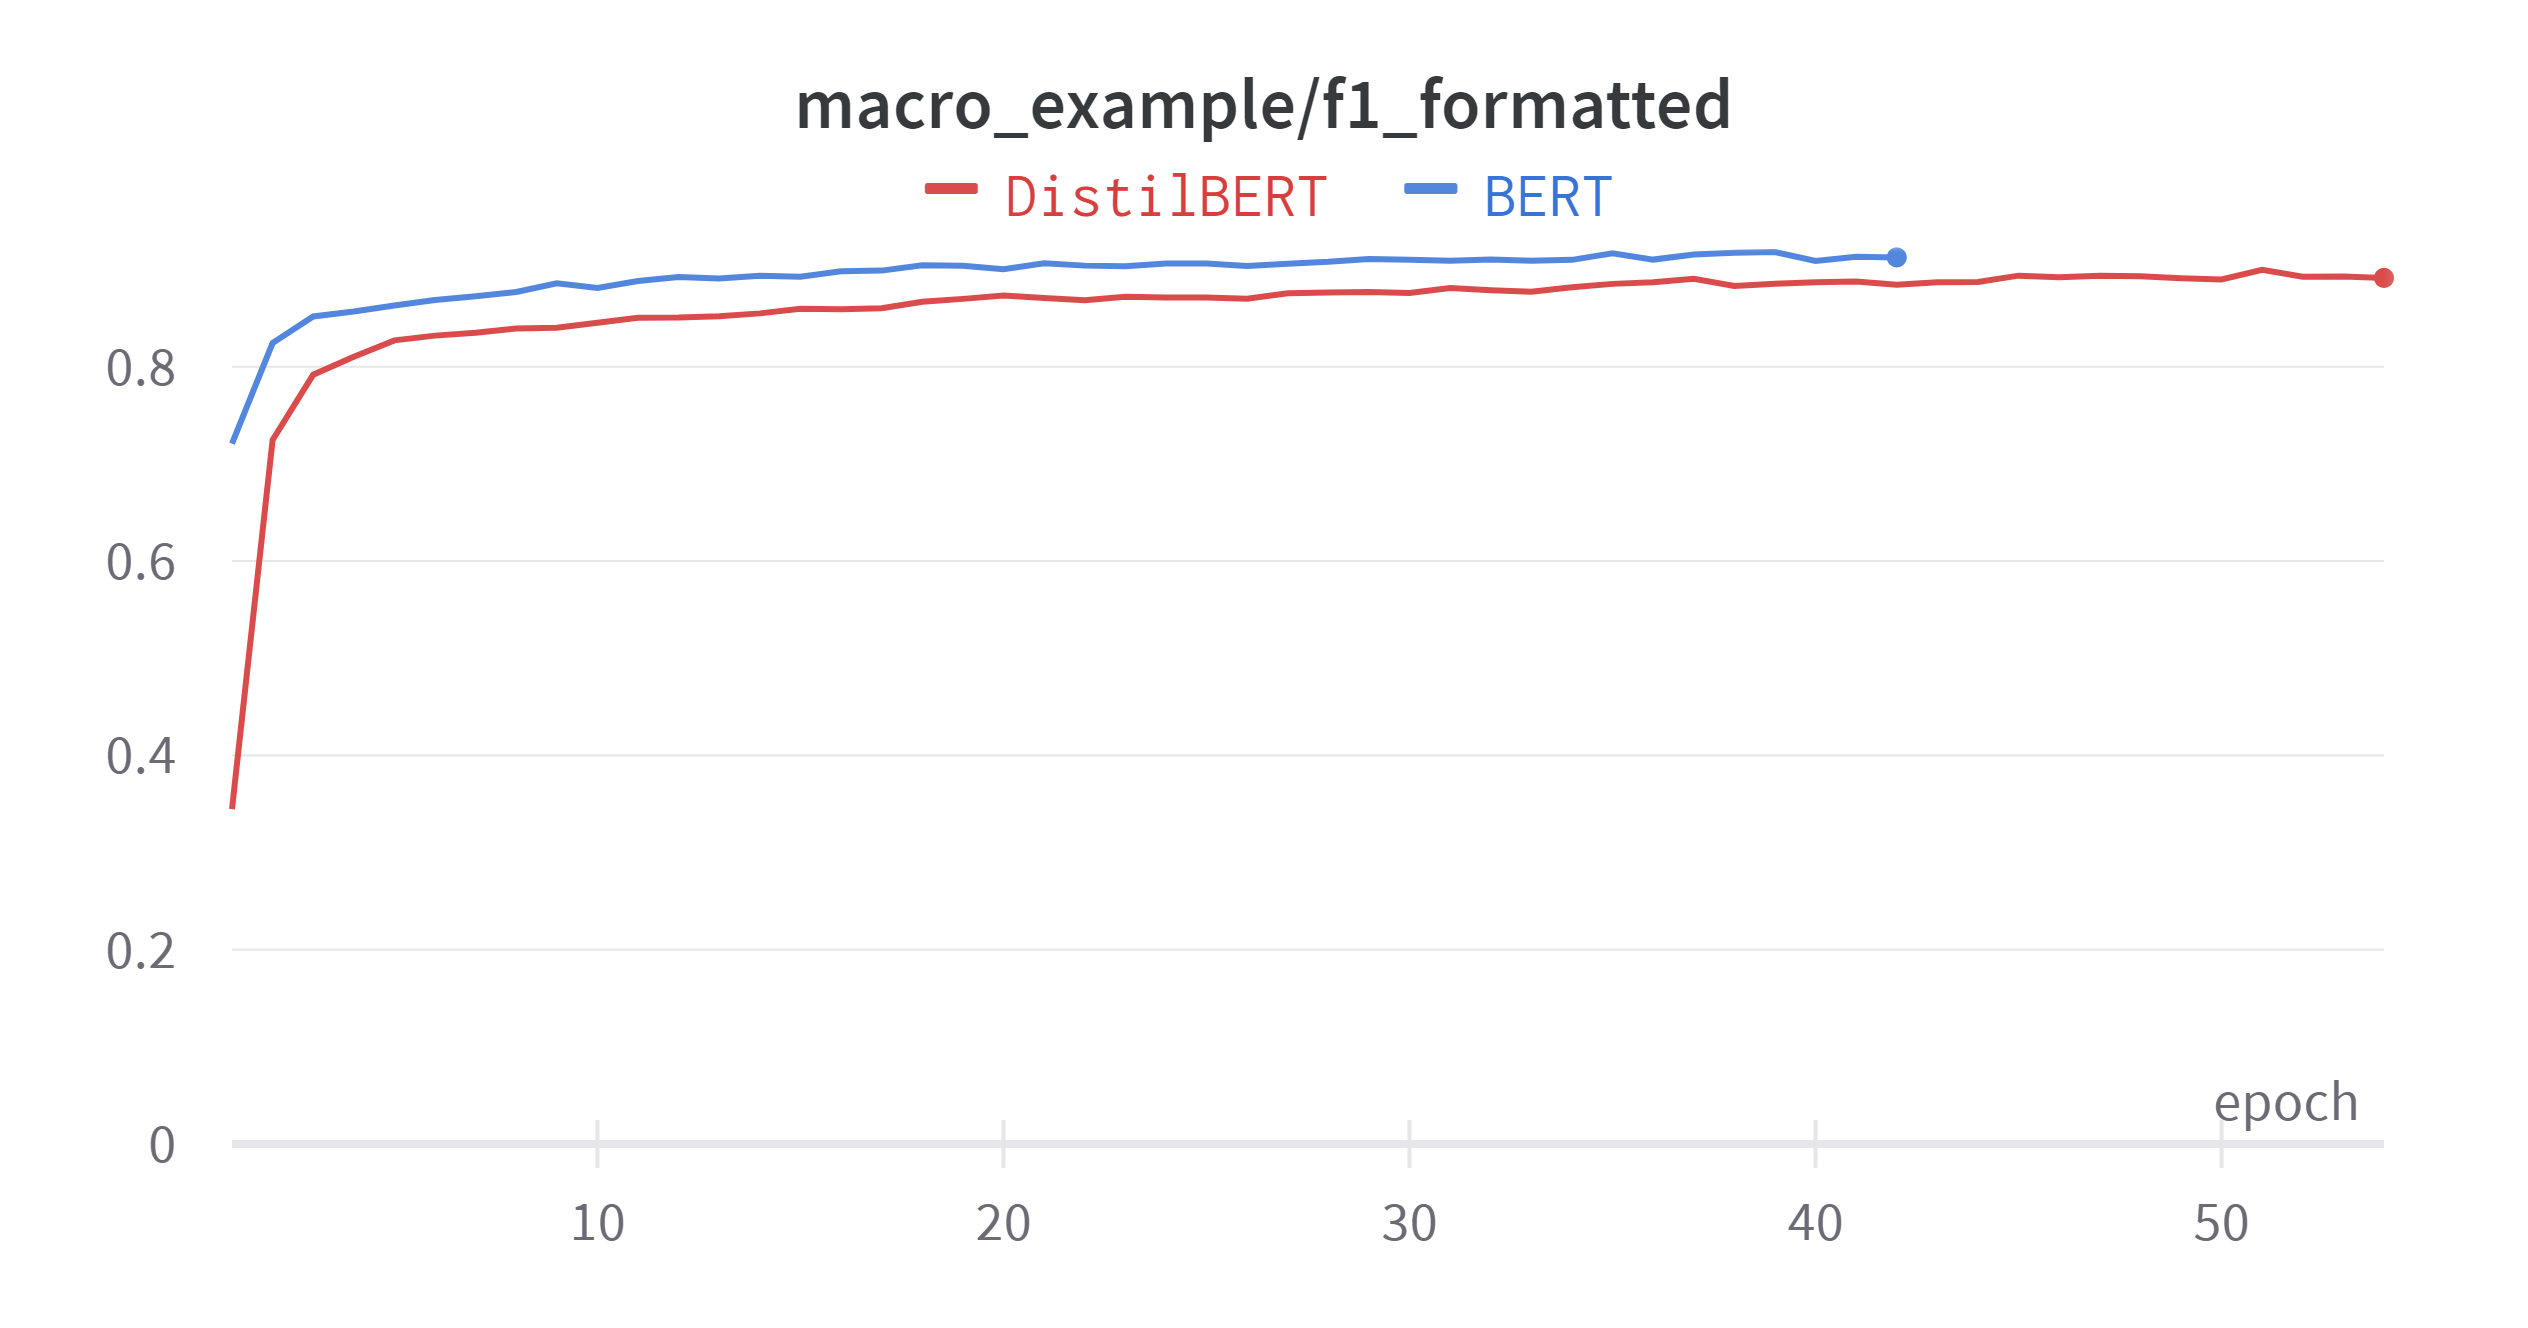
\includegraphics[width=.8\linewidth]{figures/wandb_figer_baseline_distilbert_vs_bert.png}
    \caption{Baseline DistilBERT vs Baseline BERT in terms of \textit{macro f1 examples} on the dev set of FIGER}
    \label{fig:wandb_figer_baseline_distilbert_vs_bert}
\end{figure}

Now that the superiority of BERT has been confirmed, we can proceed with the comparison between the baseline and KENN-based models. In Figures~\ref{fig:wandb_figer_kenn_distilbert} and \ref{fig:wandb_figer_kenn_bert} are presented the performance obtained with DistilBERT and BERT, respectively. As we can see, the behavior of KENN is completely different depending on the encoder. Starting from DistilBERT, the initial boost given by KENN is clearly visible, especially when comparing the baseline to the Hybrid model. However, as already discussed in the quantitative analysis, this boost vanishes in the rest of the training when the models converge. When using BERT, instead, the baseline model is the one that has the best start. While Top Down has a similar training trend even at the beginning, Bottom Up and Hybrid are always inferior.

\begin{figure}[bth]
    \centering
    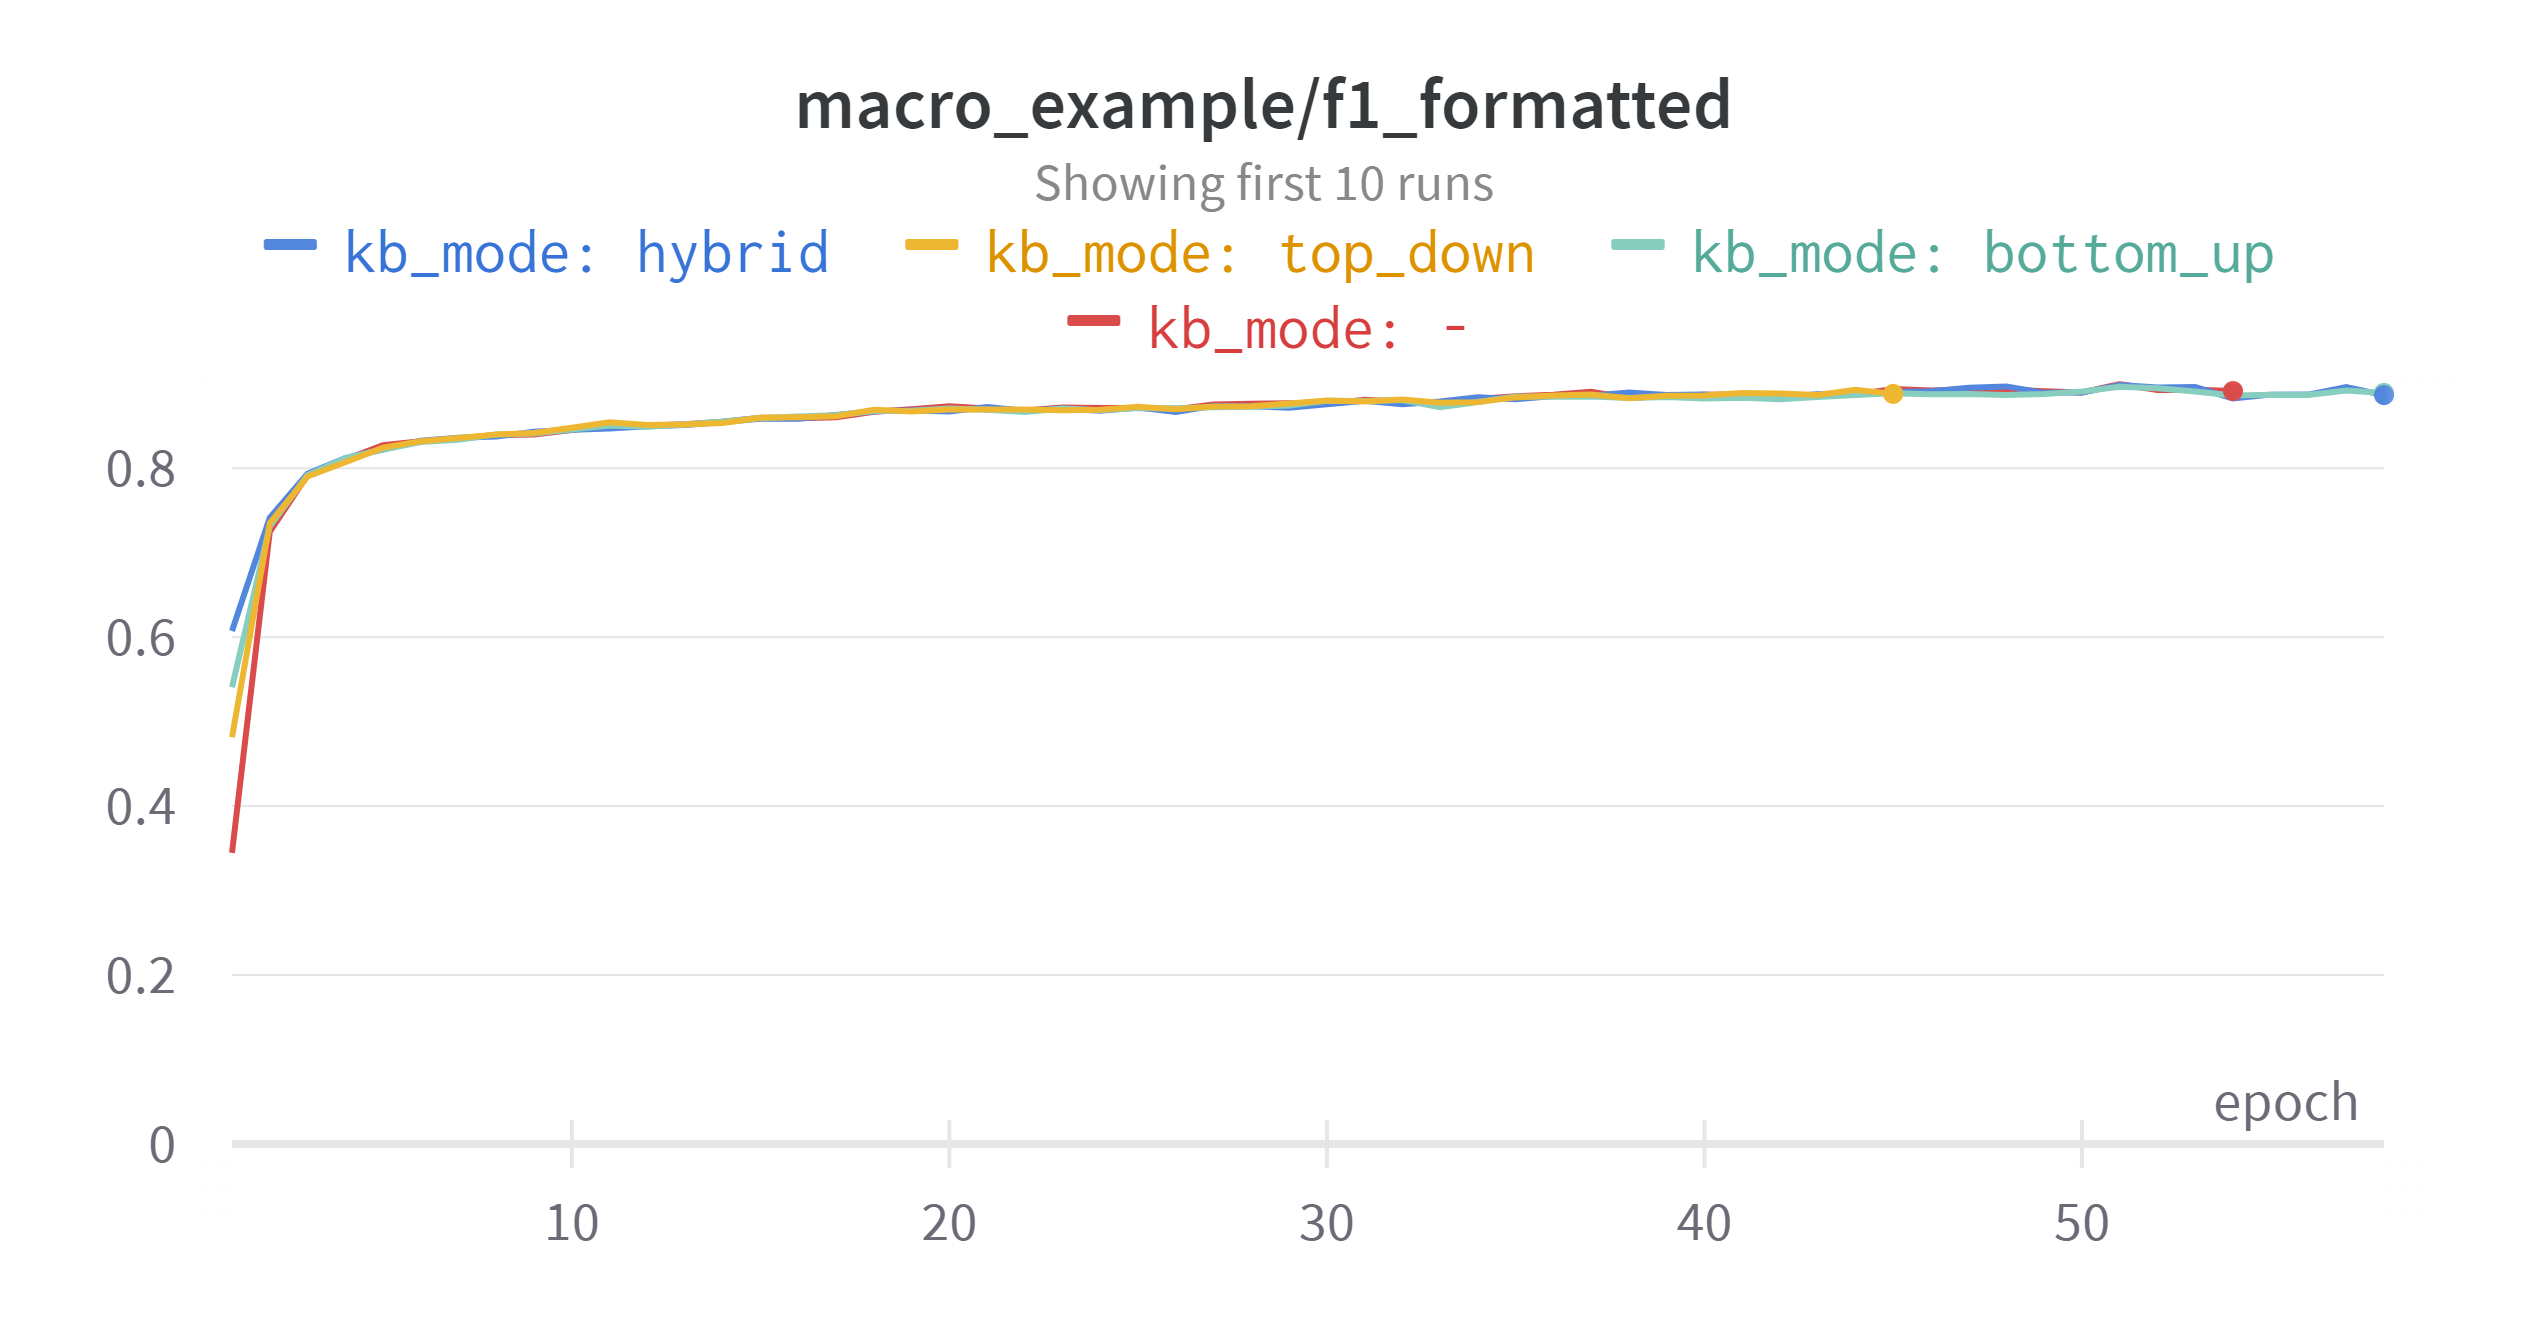
\includegraphics[width=.8\linewidth]{figures/wandb_figer_kenn_distilbert.png}
    \caption{Baseline DistilBERT vs KENN DistilBERT in terms of \textit{macro f1 examples} on the dev set of FIGER.}
    \label{fig:wandb_figer_kenn_distilbert}
\end{figure}

\begin{figure}[bth]
    \centering
    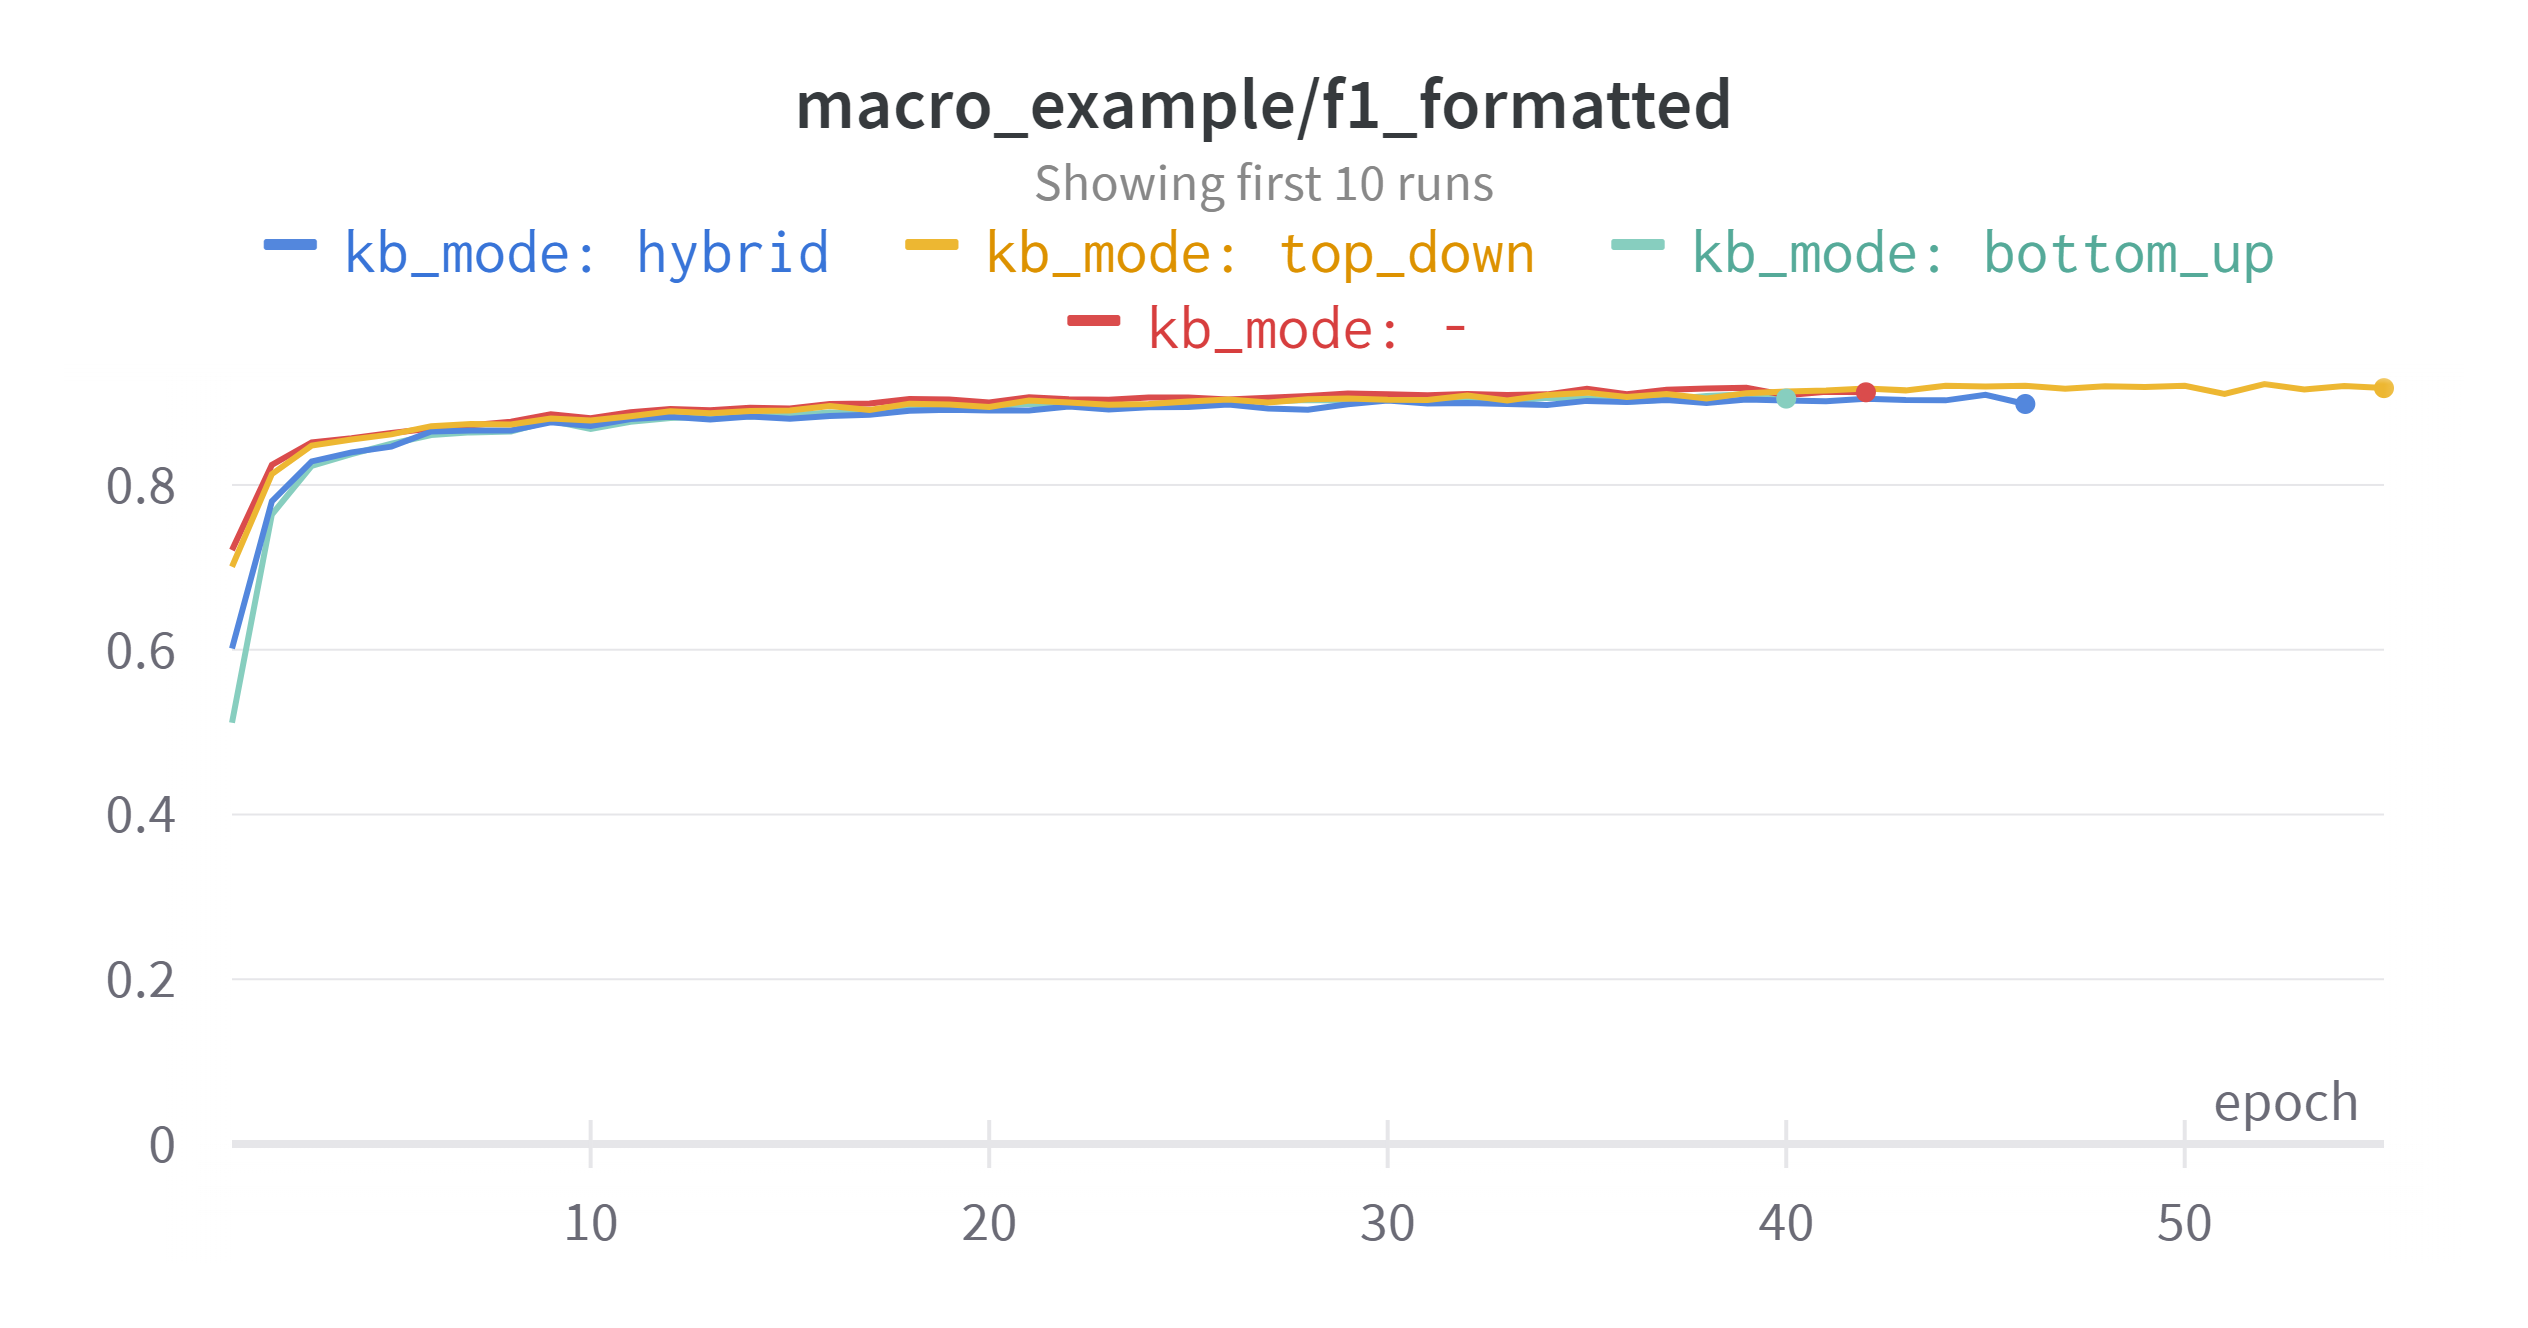
\includegraphics[width=.8\linewidth]{figures/wandb_figer_kenn_bert.png}
    \caption{Baseline BERT vs KENN BERT in terms of \textit{macro f1 examples} on the dev set of FIGER.}
    \label{fig:wandb_figer_kenn_bert}
\end{figure}




\subsubsection{Results on BBN}
Figure~\ref{fig:wandb_bbn_baseline_distilbert_vs_bert} compares DistilBERT and BERT when using the baseline model. Even this dataset confirmed the superiority of BERT, which reached the score of 0.9047, while DistilBERT's score is 0.8845.

\begin{figure}[bth]
    \centering
    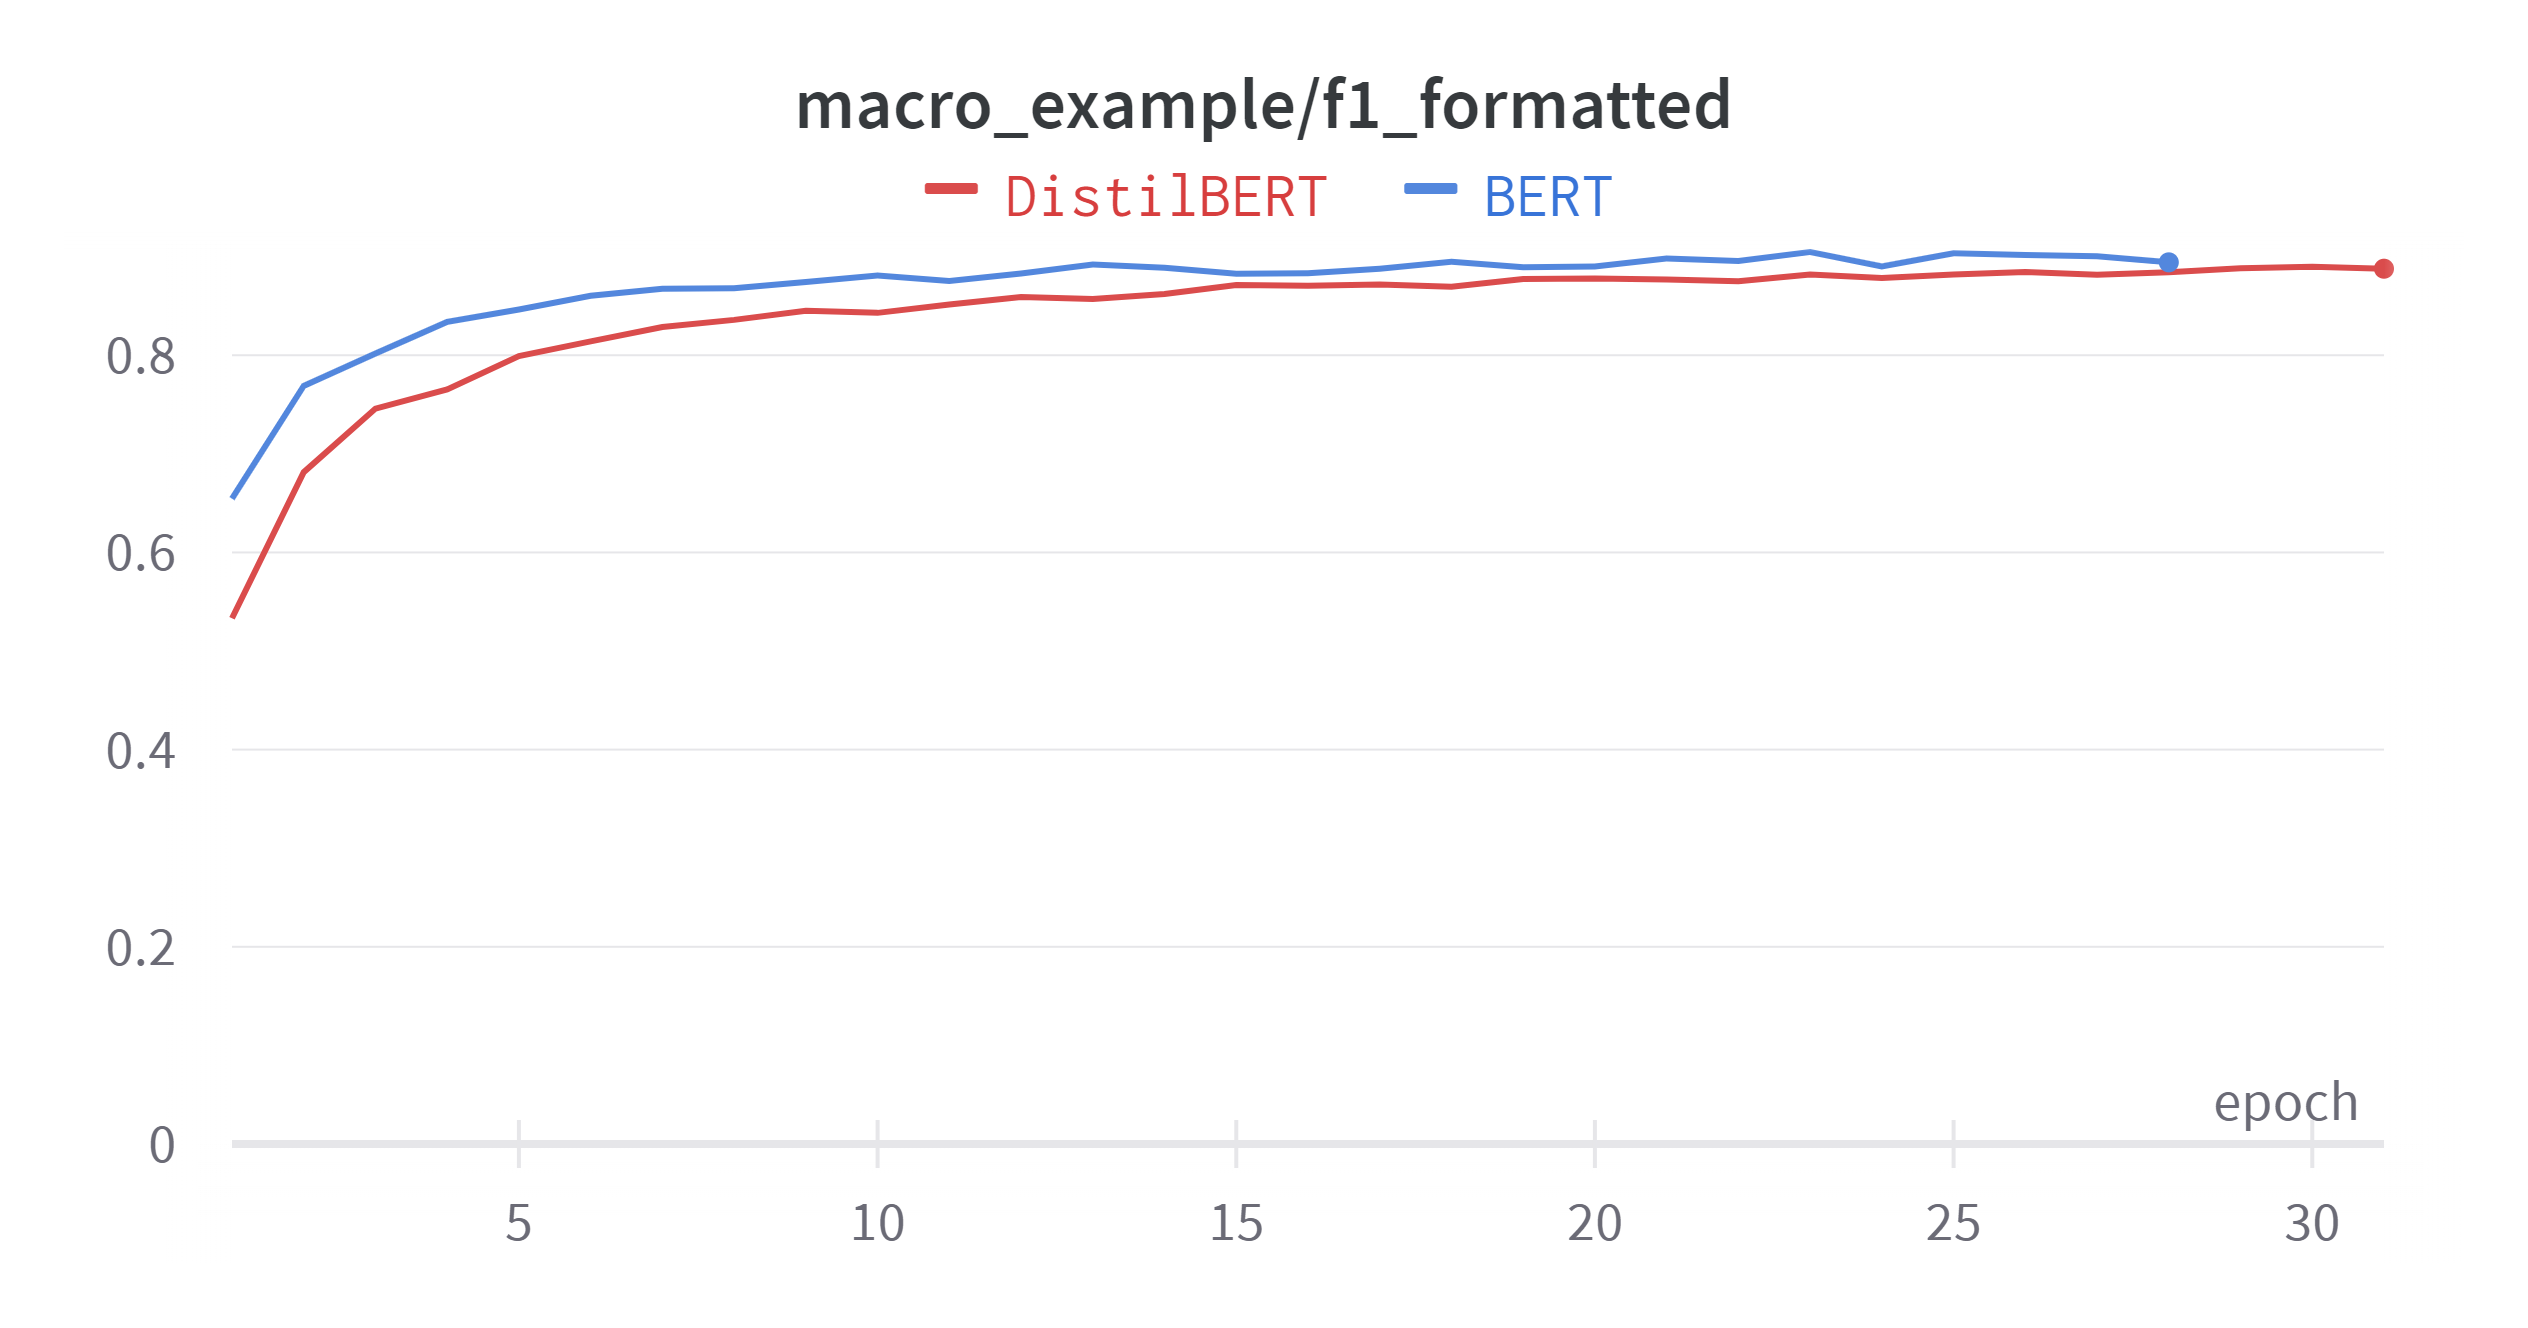
\includegraphics[width=.8\linewidth]{figures/wandb_bbn_baseline_distilbert_vs_bert.png}
    \caption{Baseline DistilBERT vs Baseline BERT in terms of \textit{macro f1 examples} on the dev set of BBN.}
    \label{fig:wandb_bbn_baseline_distilbert_vs_bert}
\end{figure}

The trends of KENN-based models compared to the baseline when using DistilBERT and BERT are available in Figures~\ref{fig:wandb_bbn_kenn_distilbert} and \ref{fig:wandb_bbn_kenn_bert}, respectively. Looking at the graphs, we can make the same observation done for FIGER: the logical knowledge gives an initial boost only when using DistilBERT. Moving on to BERT, except Bottom Up, which has a slower start, the other models have very similar training trends.

\begin{figure}[bth]
    \centering
    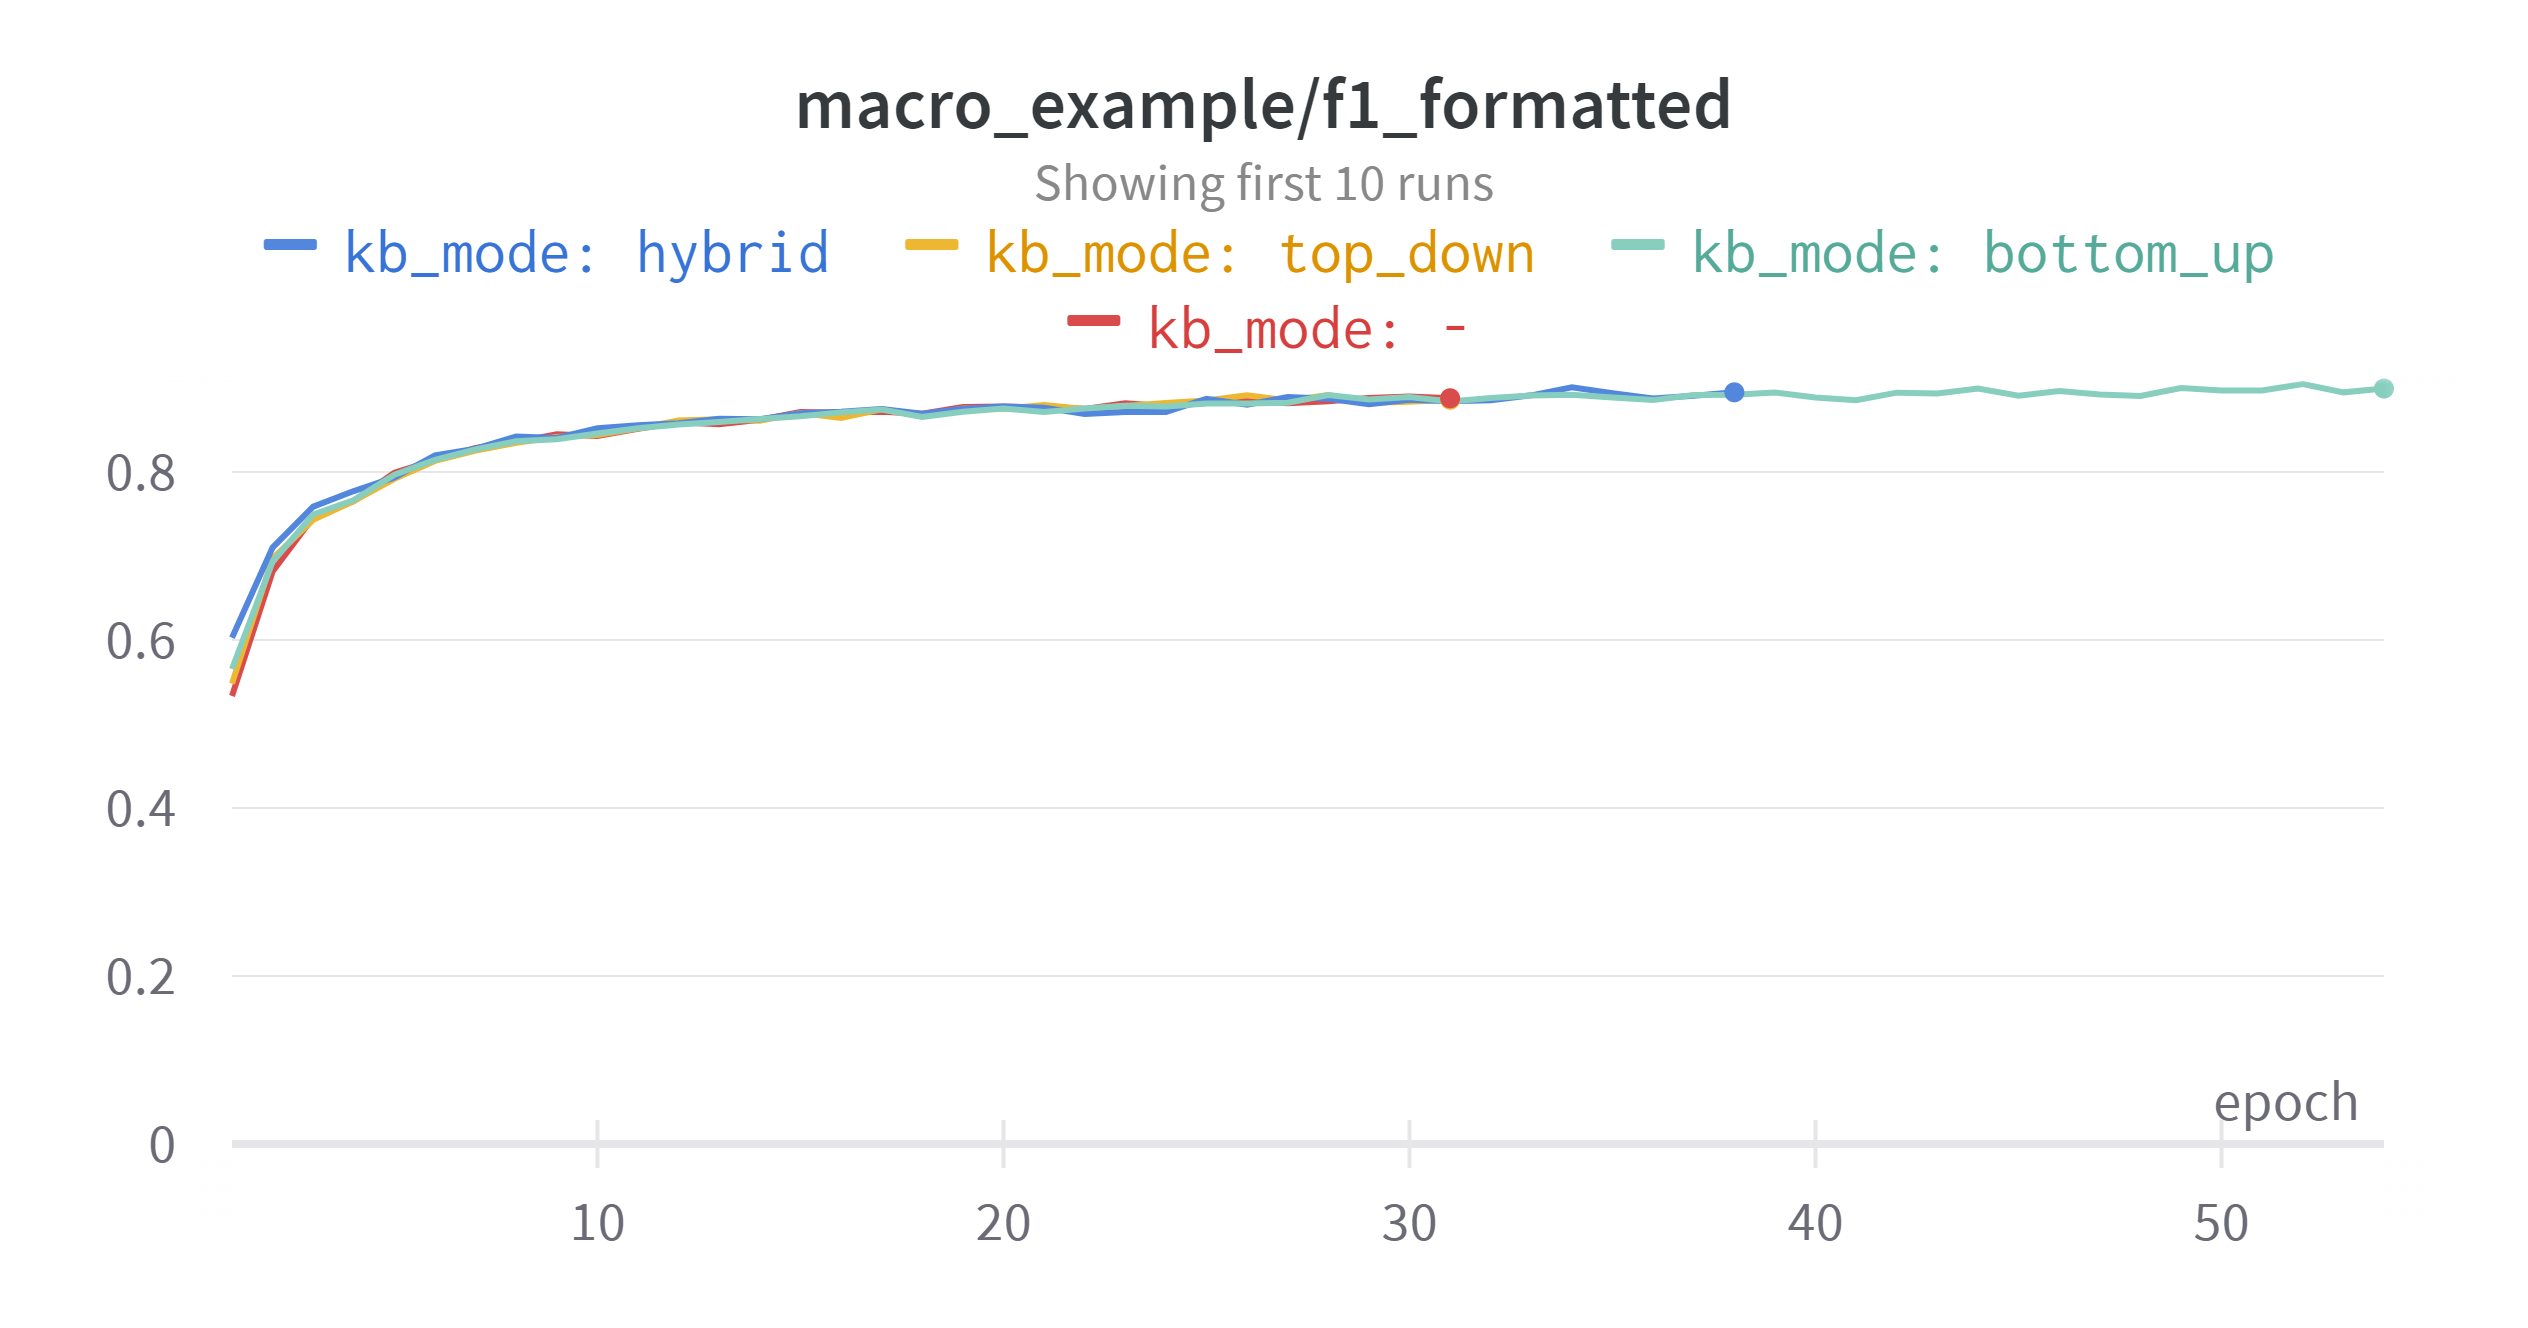
\includegraphics[width=.8\linewidth]{figures/wandb_bbn_kenn_distilbert.png}
    \caption{Baseline DistilBERT vs KENN DistilBERT in terms of \textit{macro f1 examples} on the dev set of BBN.}
    \label{fig:wandb_bbn_kenn_distilbert}
\end{figure}

\begin{figure}[bth]
    \centering
    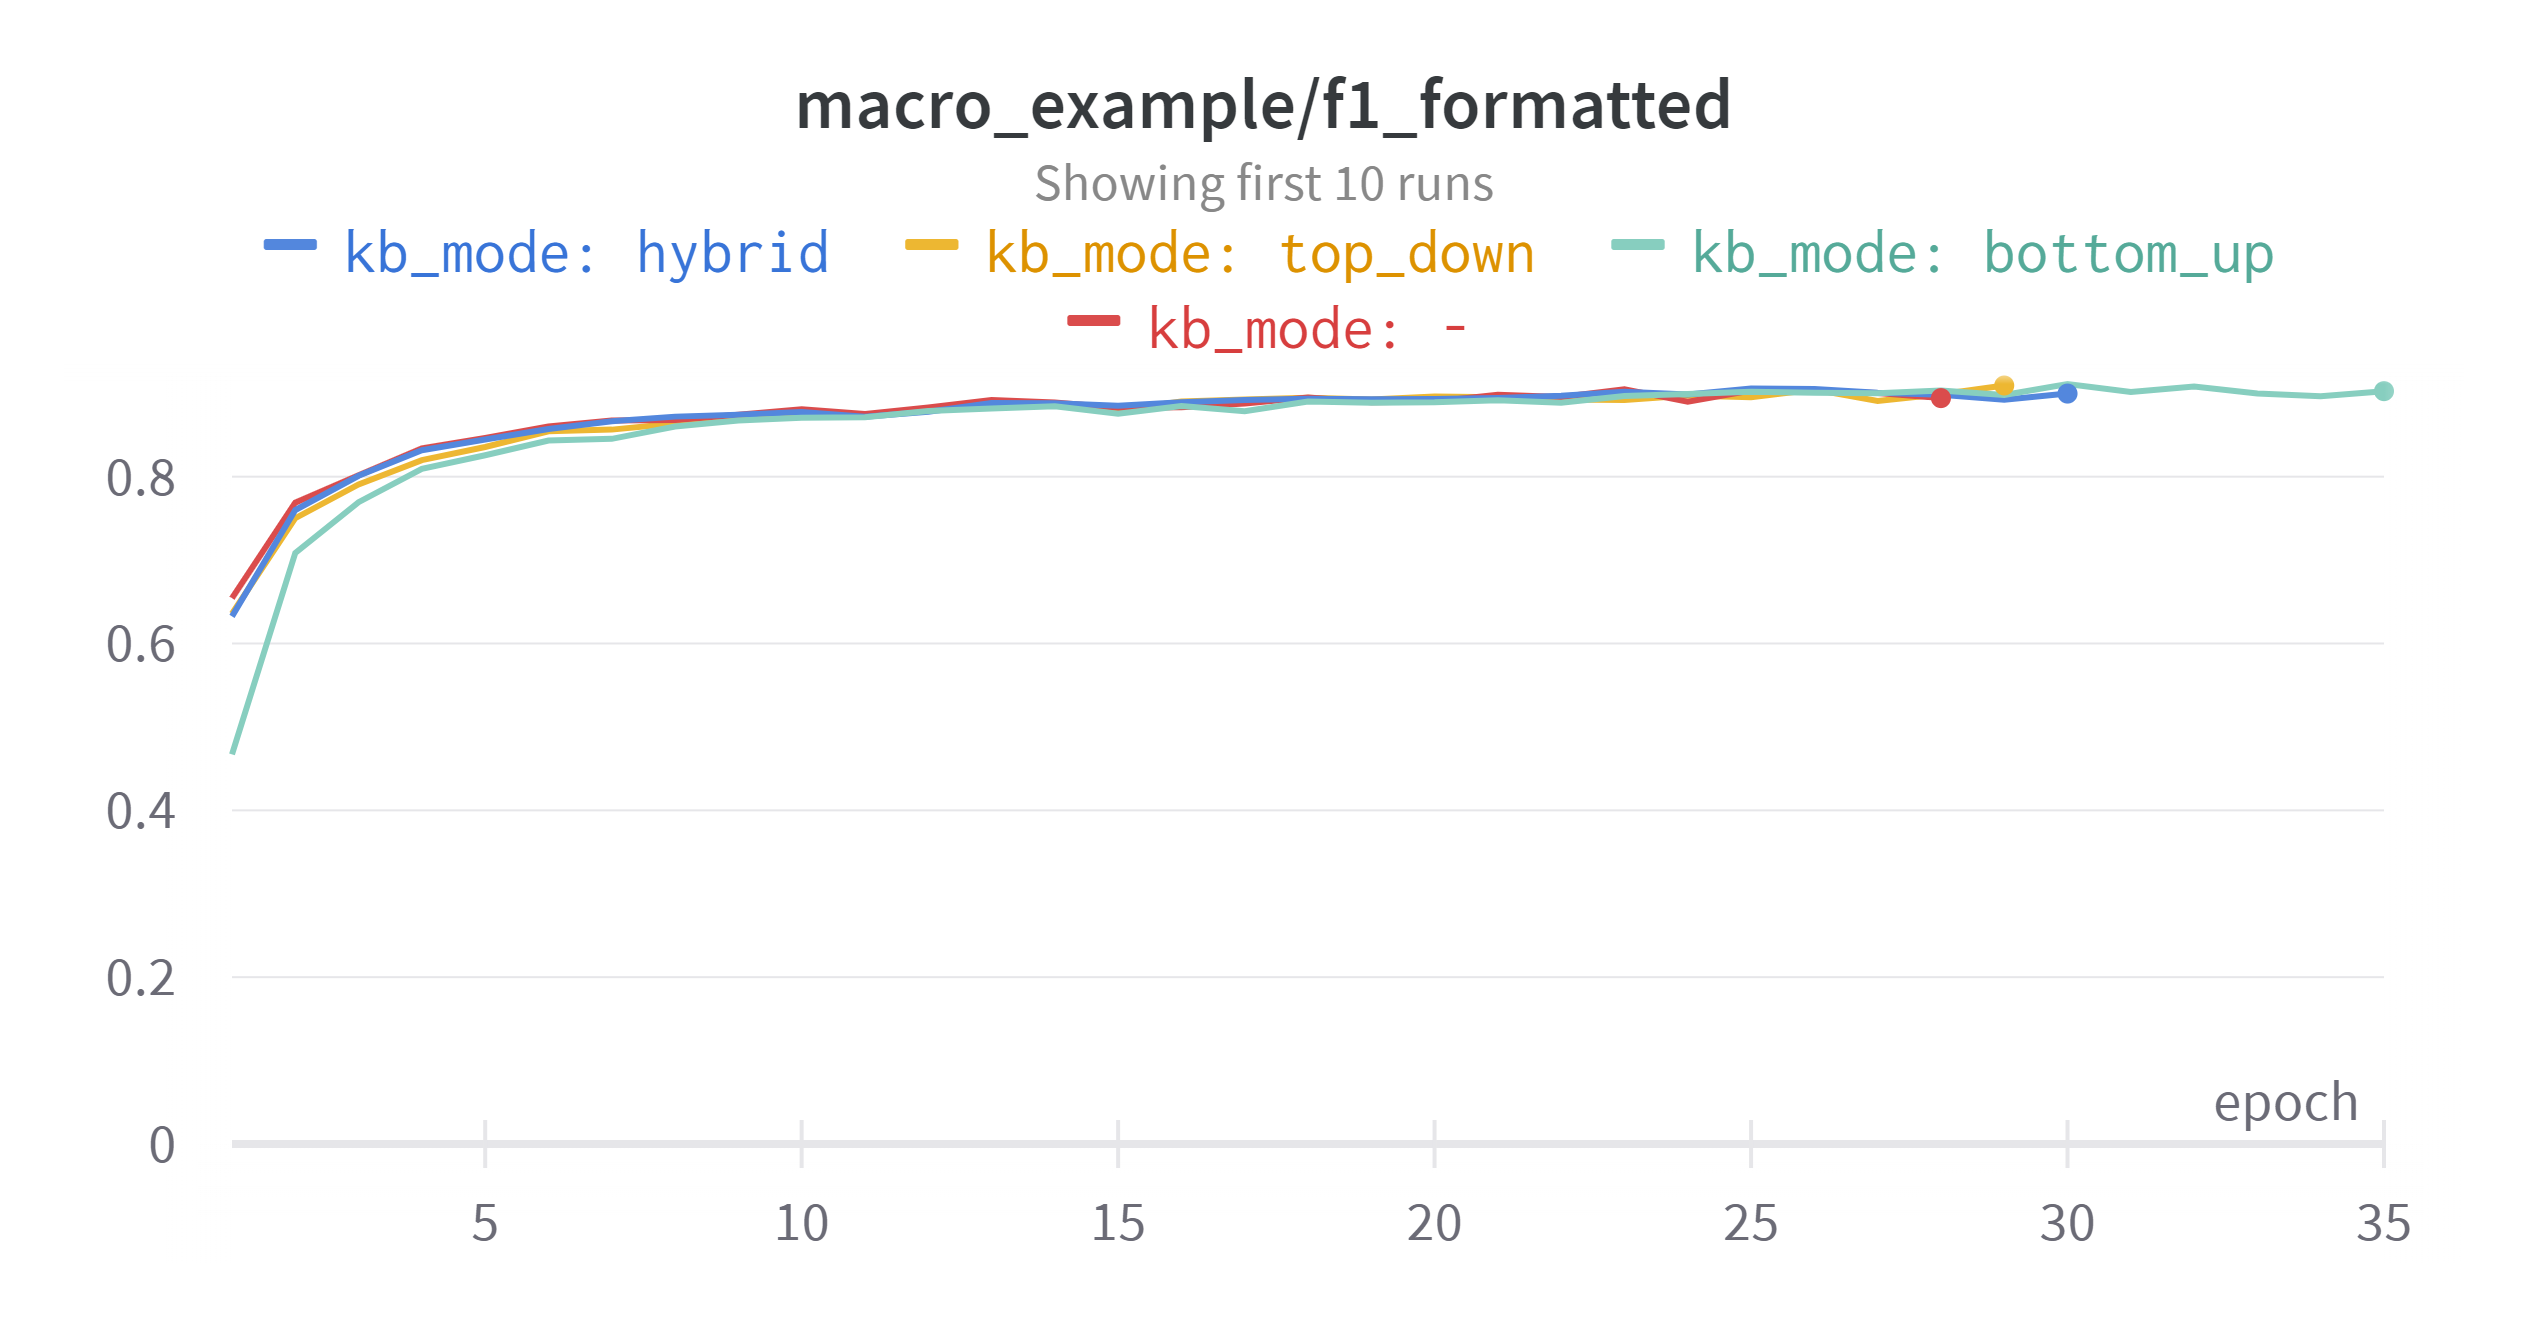
\includegraphics[width=.8\linewidth]{figures/wandb_bbn_kenn_bert.png}
    \caption{Baseline BERT vs KENN BERT in terms of \textit{macro f1 examples} on the dev set of BBN.}
    \label{fig:wandb_bbn_kenn_bert}
\end{figure}

\subsubsection{Conclusion}
The results obtained on the two datasets highlighted that the benefits of the logical knowledge are visible only in the early stage of the DistilBERT-based models. The fact that KENN worsened the performance of the BERT-based models was quite unexpected. Except for the Top Down mode, it seems that the injection of logical knowledge disturbed the learning process of the other models, especially at the beginning of the training. An explanation for this behavior can be found in the words of KENN's authors, which said that KENN has more difficulties when integrated into neural networks that are already capable to satisfy the provided clauses, since any bias is introduced towards their satisfaction~\cite{daniele2021neural}.

In our case, we observed that the performance of the baseline model was substantially improved when using BERT. For this reason, it may be possible that BERT, which provides a richer text representation than DistilBERT, is already able to implicitly learn from data the hierarchical information without the need for logical knowledge. Furthermore, we can think about the differences between the KB modes to explain why Top Down has higher performance than Bottom Up: while the knowledge provided by a Bottom Up clause could be learned from data (i.e., the model learns that a subtype always co-occur with its supertype), Top Down clauses could introduce more bias into the learning process, thus adding new solutions to the Hypothesis Space as said in~\cite{daniele2021neural}.
\subsection{KENN with multiloss function}
In previous experiments, it has been observed that the pre-KENN network adapts to the presence of KENN regardless of the parameters configuration. From these results comes the intuition to make the pre-KENN network more independent, with the purpose of exploiting the logical knowledge more effectively. To achieve this, the idea is to define a custom multiloss function to simultaneously improve the quality of the pre-KENN and post-KENN predictions.

%\subsubsection{Multiloss function}
The proposed multiloss function is computed by combining the Binary Cross-Entropy (BCE) loss values obtained from the pre-KENN and post-KENN preactivations. To make it possible, the model has been adapted to provide two outputs: one before and one after KENN's layer. The goal is to optimize the post-KENN predictions while preserving a discrete quality of pre-KENN predictions. The final loss is computed by the convex combination of the two losses whose influences are regulated by the parameter $ \alpha $. The resulting formula is the following:

% \begin{gather*}
%     L(y_{pred},y_{true}) = \alpha \cdot BCE(y_{prekenn}, y_{true}) + (1 - \alpha) \cdot BCE(y_{postkenn}, y_{true})
% \end{gather*}

\begin{gather*}
    L(Y, Y', Y_{t}) = \alpha \cdot BCE(Y, Y_{t}) + (1 - \alpha) \cdot BCE(Y', Y_{t})
\end{gather*}
where $Y$ denotes the pre-KENN predictions, $Y'$ the post-KENN predictions, and $Y_{t}$ the values of the ground truth.


\subsubsection{Setup}
The models involved in this experiment are trained following the \textit{Setup B}. The configuration of the other parameters is the following:
\begin{itemize}
    \item \textbf{KB modes:} Bottom Up and Top Down
    \item \textbf{initial clause weights:} 0.5 and variable\footnote{With the term ``variable" we mean that each clause can be initialized with a different value. The original implementation of KENN did not contemplate this possibility when setting clause weights as learnable parameters, so we introduced a small modification to make it possible.}
    \item \textbf{learnable clause weights}
    \item \textbf{encoder:} DistilBERT and BERT, with adapters
    \item \textbf{loss function:} multiloss with $\alpha = 0.5$
\end{itemize}
The total number of configurations obtained by varying these parameters is 8. Since the pre-KENN network is expected to be less influenced by KENN, the clause weights are set as learnable parameters with small initial values to start with a soft influence and let the network establish the relevance of each clause. Indeed, the choice of learnable clause weights allows us to study the weight evolution during the epochs and determine which are the most useful and the least useful clauses. Furthermore, for each clause, the types that are the antecedents of an implication rule (i.e., the types that propagate the information and uniquely characterize the used KBs) have been studied to look for some recurring behavioral patterns. The \textit{Hybrid} mode is excluded from this study because it involves the same clauses of \textit{Bottom Up} and \textit{Top Down}, but with the addition of noise due to the presence of conflicts. For this reason, it would not have been possible to carry out an accurate analysis.

\subsubsection{Results on FIGER}
\paragraph{DistilBERT}
The results obtained using DistilBERT as encoder show some very interesting behaviors of the clause weights. Starting from the Bottom Up, if we look at the distribution of final clause weights in Figure~\ref{fig:weight_distrib_distilbert_figer_bu_multiloss} we can see that almost every weight decreases its initial value. This attitude is not observable in Figure~\ref{fig:weight_distrib_distilbert_figer_bu_learnable} when using KENN with a standard loss and learnable weights. If we look at the figure, we can see widely different results since almost every weight increases its starting value. The same trend is detectable in the Top Down mode, as shown in Figure~\ref{fig:weight_distrib_distilbert_figer_td}.

\begin{figure}[bth]
     \centering
     \begin{subfigure}[b]{0.45\textwidth}
         \centering
         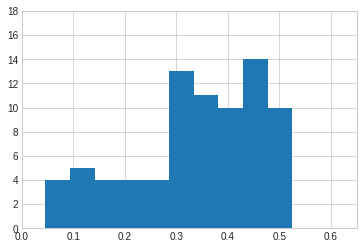
\includegraphics[width=\textwidth]{figures/weight_distrib_distilbert_figer_bu_multiloss.png}
         \caption{Multiloss model - Epoch 55 (563K examples)}
         \label{fig:weight_distrib_distilbert_figer_bu_multiloss}
     \end{subfigure}
     \hspace{10px}
     \begin{subfigure}[b]{0.45\textwidth}
         \centering
         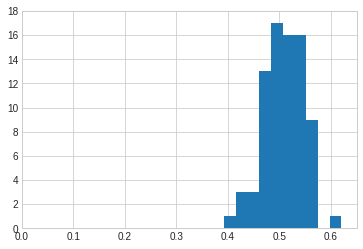
\includegraphics[width=\textwidth]{figures/weight_distrib_distilbert_figer_bu_learnable.png}
         \caption{Standard loss model - Epoch 42 (430K examples)}
         \label{fig:weight_distrib_distilbert_figer_bu_learnable}
     \end{subfigure}
    \caption{Distributions of the final learned clause weights for the Bottom Up KB mode using DistilBERT-based models - FIGER}
    \label{fig:weight_distrib_distilbert_figer_bu}
\end{figure}

\begin{figure}[bth]
     \centering
     \begin{subfigure}[b]{0.45\textwidth}
         \centering
         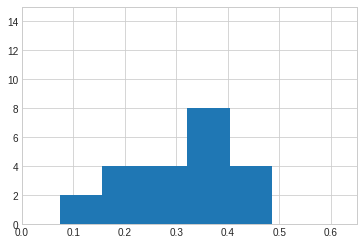
\includegraphics[width=\textwidth]{figures/weight_distrib_distilbert_figer_td_multiloss.png}
         \caption{Multiloss model - Epoch 42 (430K examples)}
         \label{fig:weight_distrib_distilbert_figer_td_multiloss}
     \end{subfigure}
     \hspace{10px}
     \begin{subfigure}[b]{0.45\textwidth}
         \centering
         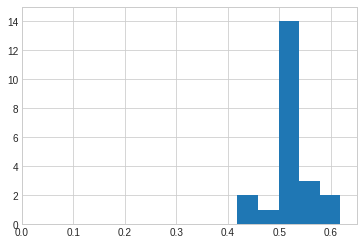
\includegraphics[width=\textwidth]{figures/weight_distrib_distilbert_figer_td_learnable.png}
         \caption{Standard loss model - Epoch 39 (399K examples)}
         \label{fig:weight_distrib_distilbert_figer_td_learnable}
     \end{subfigure}
    \caption{Distributions of the final learned clause weights for the Top Down KB mode using DistilBERT-based models - FIGER}
    \label{fig:weight_distrib_distilbert_figer_td}
\end{figure}


Moving on to the analysis of the types involved in the clauses we can observe an unexpected behavior. For both Bottom Up and Top Down modes, this study intercepts a remarkable fact: the more a type occurs in the training set, the lower the final weight of its clause. The few clauses that preserve a high weight are those whose antecedents are the rarest in the dataset. Starting from the Bottom Up mode, we can see in Figure~\ref{fig:weight_freq_distilbert_figer_bu_multiloss} a graph showing the relation between the final weight and the frequency of each type S. Looking at the figure, we can clearly observe that there is a strong correlation between weight and frequency. Indeed, the correlation coefficient is -0.77. The Top Down mode (Figure~\ref{fig:weight_freq_distilbert_figer_td_multiloss}) also presents a negative correlation, this time of -0.68 with respect to the frequencies of types F.
%This behavior may be explained by the fact that KENN introduces too much noise to types that the network can already predict discretely without the use of knowledge. 

\begin{figure}[bth]
     \centering
     \begin{subfigure}[b]{0.7\textwidth}
         \centering
         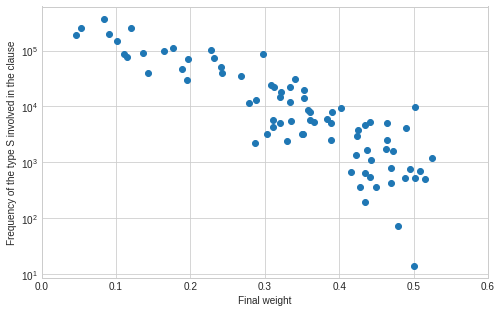
\includegraphics[width=\textwidth]{figures/weight_freq_distilbert_figer_bu_multiloss.png}
         \caption{Bottom Up - Epoch 55 (563K examples)}
         \label{fig:weight_freq_distilbert_figer_bu_multiloss}
         \vspace{10px}
     \end{subfigure}
     \begin{subfigure}[b]{0.7\textwidth}
         \centering
         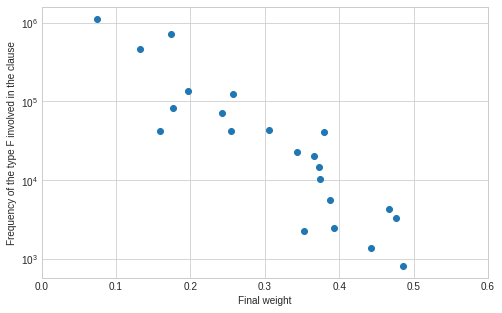
\includegraphics[width=\textwidth]{figures/weight_freq_distilbert_figer_td_multiloss.png}
         \caption{Top Down - Epoch 42 (430K examples)}
         \label{fig:weight_freq_distilbert_figer_td_multiloss}
     \end{subfigure}
    \caption{Relation between types frequency (log scale) and final clause weights of multiloss models using DistilBERT - FIGER}
    \label{fig:weight_freq_distilbert_figer}
\end{figure}

By inspecting the weight evolution over the epochs, it emerged that the clause weights keep decreasing until the last epoch, but it is not known for how long they would have continued. To observe in advance the effect of higher epochs and see if some clauses would have reached a weight close to zero, new models were trained starting from variable weights assigned with respect to the frequency of the antecedents of each clause. Clauses involving popular types were assigned a weight of 0.2, while the others kept a weight of 0.5. The weight assignment is based on a frequency threshold of 70K for Bottom Up and 50K for Top Down\footnote{the values are chosen by observing the graphs, without formalizing a mathematical criterion}. The results of these runs are shown in Figure~\ref{fig:weight_freq_distilbert_figer_bu_multiloss_variable} and Figure~\ref{fig:weight_freq_distilbert_figer_td_multiloss_variable} for Bottom Up and Top Down, respectively. As we can see, most clause weights decreased their values even when starting from lower initial values.
%However, by analyzing the weight evolution, it emerged that their decrease over the epochs was slowed down. The reason for this fact is that clauses now have less influence on the final prediction, so they are penalized in a minor way by the loss function.

\begin{figure}[bth]
     \centering
     \begin{subfigure}[b]{0.7\textwidth}
         \centering
         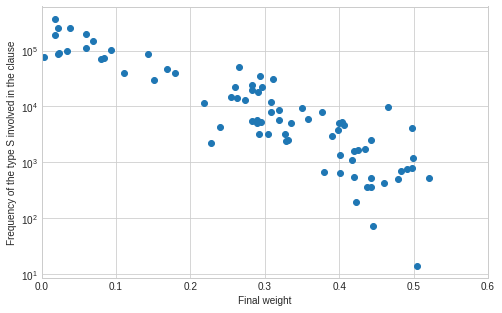
\includegraphics[width=\textwidth]{figures/weight_freq_distilbert_figer_bu_multiloss_variable.png}
         \caption{Bottom Up - Epoch 71 (727K examples)}
         \label{fig:weight_freq_distilbert_figer_bu_multiloss_variable}
         \vspace{10px}
     \end{subfigure}
     \begin{subfigure}[b]{0.7\textwidth}
         \centering
         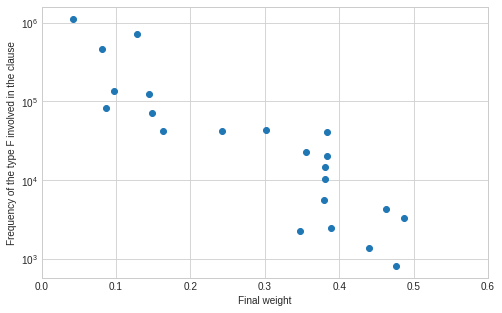
\includegraphics[width=\textwidth]{figures/weight_freq_distilbert_figer_td_multiloss_variable.png}
         \caption{Top Down - Epoch 42 (430K examples)}
         \label{fig:weight_freq_distilbert_figer_td_multiloss_variable}
     \end{subfigure}
    \caption{Relation between types frequency (log scale) and final clause weights of multiloss models using DistilBERT and \textit{variable} clause weights - FIGER}
    \label{fig:weight_freq_distilbert_figer_variable}
\end{figure}

\paragraph{BERT}
The experiments performed using BERT showed an identical behavior. The results obtained with weights set to 0.5 for every clause are shown in Figure~\ref{fig:weight_freq_bert_figer}. The correlation between weight and frequency is similar (-0.76 in Bottom Up, -0.74 in Top Down) as well as the weight evolution during the epochs. The only difference with respect to DistilBERT is that BERT needs fewer epochs to converge, so its weights have decreased less as it performed fewer backward propagation operations. Much lower weights are reached when using the setup with variable weights as reported in Figure~\ref{fig:weight_freq_bert_figer_variable}.

\begin{figure}[bth]
     \centering
     \begin{subfigure}[b]{0.7\textwidth}
         \centering
         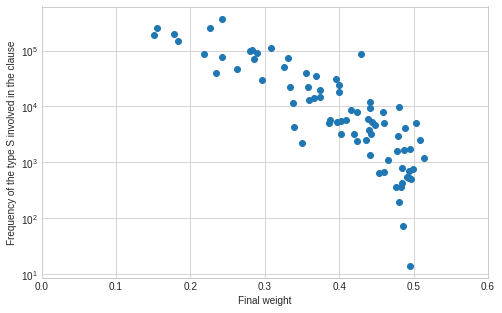
\includegraphics[width=\textwidth]{figures/weight_freq_bert_figer_bu_multiloss.png}
         \caption{Bottom Up - Epoch 35 (358K training examples)}
         \label{fig:weight_freq_bert_figer_bu_multiloss}
         \vspace{10px}
     \end{subfigure}
     \begin{subfigure}[b]{0.7\textwidth}
         \centering
         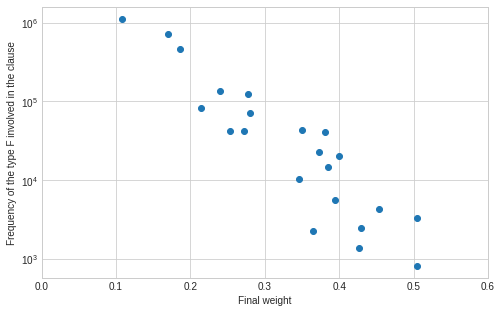
\includegraphics[width=\textwidth]{figures/weight_freq_bert_figer_td_multiloss.png}
         \caption{Top Down - Epoch 35 (358K training examples)}
         \label{fig:weight_freq_bert_figer_td_multiloss}
     \end{subfigure}
    \caption{Relation between types frequency (log scale) and final clause weights of multiloss models using BERT - FIGER}
    \label{fig:weight_freq_bert_figer}
\end{figure}

\begin{figure}[bth]
     \centering
     \begin{subfigure}[b]{0.7\textwidth}
         \centering
         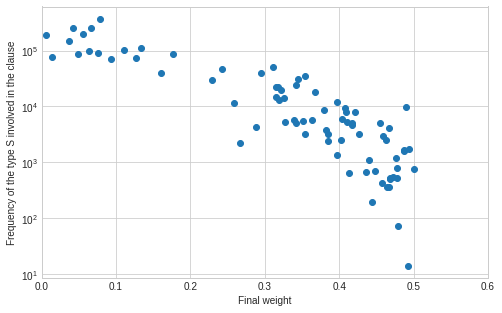
\includegraphics[width=\textwidth]{figures/weight_freq_bert_figer_bu_multiloss_variable.png}
         \caption{Bottom Up - Epoch 49 (501K training examples)}
         \label{fig:weight_freq_bert_figer_bu_multiloss_variable}
         \vspace{10px}
     \end{subfigure}
     \begin{subfigure}[b]{0.7\textwidth}
         \centering
         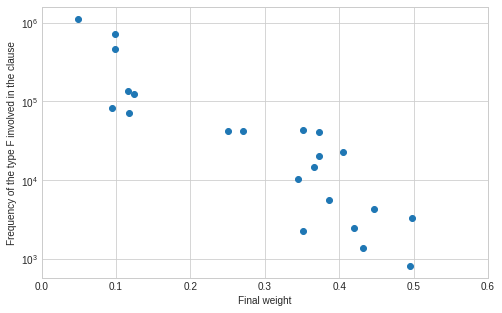
\includegraphics[width=\textwidth]{figures/weight_freq_bert_figer_td_multiloss_variable.png}
         \caption{Top Down - Epoch 33 (337K training examples)}
         \label{fig:weight_freq_bert_figer_td_multiloss_variable}
     \end{subfigure}
    \caption{Relation between types frequency (log scale) and final clause weights of multiloss models using BERT and \textit{variable} clause weights - FIGER}
    \label{fig:weight_freq_bert_figer_variable}
\end{figure}


\subsubsection{Results on BBN}
The experiments on BBN were performed directly on BERT. In Figure~\ref{fig:weight_freq_bert_bbn} are represented the graphs of weights and frequencies using the same weight for each clause. The correlation coefficients of the Bottom Up and Top Down modes are -0.73 and -0.55, respectively. The results obtained after repeating the experiments using variable weights are shown in Figure~\ref{fig:weight_freq_bert_bbn_variable}. The weight assignment is based on a frequency threshold of 1700 for Bottom Up and 1500 for Top Down\footnote{the values are chosen by observing the graphs, without formalizing a mathematical criterion}. Looking at the graphs, it is possible to observe that most of the weights continued to decrease.

\begin{figure}
     \centering
     \begin{subfigure}[b]{0.7\textwidth}
         \centering
         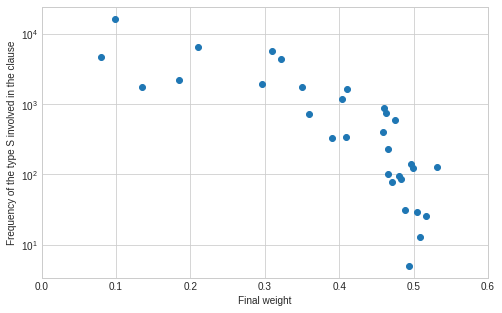
\includegraphics[width=\textwidth]{figures/weight_freq_bert_bbn_bu_multiloss.png}
         \caption{Bottom Up - Epoch 28 (286K training examples)}
         \label{fig:weight_freq_bert_bbn_bu_multiloss}
         \vspace{10px}
     \end{subfigure}
     \begin{subfigure}[b]{0.7\textwidth}
         \centering
         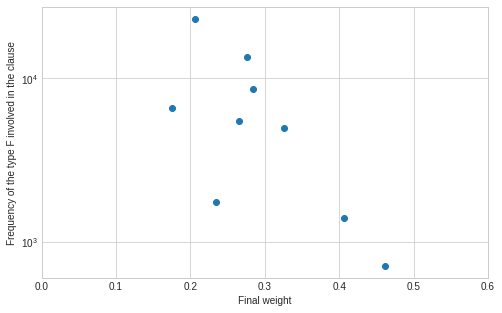
\includegraphics[width=\textwidth]{figures/weight_freq_bert_bbn_td_multiloss.png}
         \caption{Top Down - Epoch 19 (194K training examples)}
         \label{fig:weight_freq_bert_bbn_td_multiloss}
     \end{subfigure}
    \caption{Relation between types frequency (log scale) and final clause weights of multiloss models using BERT - BBN}
    \label{fig:weight_freq_bert_bbn}
\end{figure}

\begin{figure}
     \centering
     \begin{subfigure}[b]{0.7\textwidth}
         \centering
         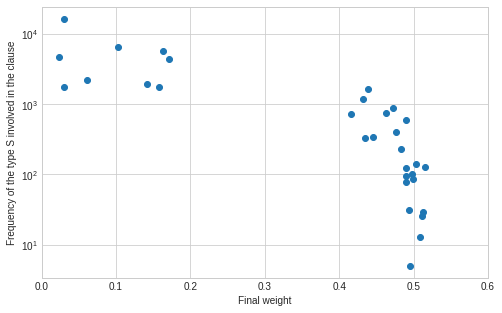
\includegraphics[width=\textwidth]{figures/weight_freq_bert_bbn_bu_multiloss_variable.png}
         \caption{Bottom Up - Epoch 19 (194K training examples)}
         \label{fig:weight_freq_bert_bbn_bu_multiloss_variable}
         \vspace{10px}
     \end{subfigure}
     \begin{subfigure}[b]{0.7\textwidth}
         \centering
         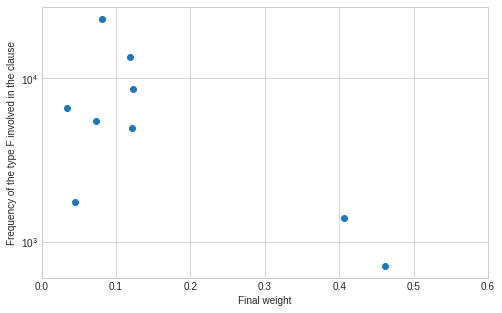
\includegraphics[width=\textwidth]{figures/weight_freq_bert_bbn_td_multiloss_variable.png}
         \caption{Top Down - Epoch 19 (194K training examples)}
         \label{fig:weight_freq_bert_bbn_td_multiloss_variable}
     \end{subfigure}
    \caption{Relation between types frequency (log scale) and final clause weights of multiloss models using BERT and \textit{variable} clause weights - BBN}
    \label{fig:weight_freq_bert_bbn_variable}
\end{figure}



\subsubsection{Conclusion}
The multiloss experiments showed that the pre-KENN network suffers the presence of some logical clauses when it is forced to not adapt its predictions to KENN. In particular, it has been possible to see that the learning process penalized clauses involving the most frequent types much more than the others. This behavior can be motivated by the fact that if a network sees a lot of instances labeled with some types, then it becomes able to correctly classify them without needing logical knowledge. For this reason, it seems that the action of KENN on frequent types is seen as noise added to the final predictions. Conversely, the enhancement of rarer types is not penalized by the learning process, so logical clauses seem to be helpful for the network when few examples labeled with those types are available. For this reason, using a multiloss setup could be a reasonable choice to exploit logical knowledge only where needed, thus avoiding having side effects on the types that are easier to predict.


\subsection{Test set evaluation} \label{test_evaluation}
The models chosen for the test set evaluation come from the multiloss experiments. Based on \textit{Setup B}, they have the following configuration:
\begin{itemize}
    \item \textbf{KB modes:} Bottom Up and Top Down
    \item \textbf{initial clause weights:} 0.5 and variable
    \item \textbf{learnable clause weights}
    \item \textbf{encoder:} BERT with adapters
    \item \textbf{loss function:} multiloss with $\alpha = 0.5$
\end{itemize}
% scelta modelli
The choice of the multiloss setup has the following reasons derived from the experimental results:
\begin{enumerate}
    \item When using a standard loss setup, the pre-KENN network adapts its predictions to the presence of KENN and achieves results that are very similar to the baseline ones. This means that KENN-based models can be seen as simple baseline models that have had different evolutions due to the noise introduced by KENN.
    \item When using a multiloss setup, the pre-KENN network avoids the adaptation thanks to the pre-KENN loss. The final clause weights will ensure that the network only uses KENN when it really needs it.
    \item The choice of variable clause weights may emphasize the effect of the multiloss on final weights, thus producing models in which the influence of KENN is slightly different.
\end{enumerate}
The test set has been evaluated using the metrics of \textit{macro f1 examples} and \textit{macro f1 classes}. The inference rules used to compute the final predictions are the \textit{threshold} and \textit{threshold or max}.

\paragraphn{Results on FIGER}
Table~\ref{tab:performance_figer} shows the results obtained on FIGER. If we look at the performance with the \textit{threshold} inference, we can see that the Top Down mode is the best in every metric. With respect to the baseline model, it gains 0.0151 on \textit{macro f1 examples} and 0.0108 on \textit{macro f1 classes}. 

KENN-based models become even more competitive when using the \textit{threshold or max} inference. In this case, the metrics obtained by Bottom Up and Top Down are quite similar. The best performance on \textit{macro f1 examples} and \textit{macro f1 classes} are reached by Bottom Up and Top Down by gaining 0.0181 and 0.0137, respectively, over the baseline. Note that by changing the inference rule, Bottom Up and Top Down increase their \textit{macro examples f1} much more than the baseline.

\begin{table}[H]
\centering
\caption{Performance of the baseline and KENN multiloss models on the test set - FIGER}
\label{tab:performance_figer}
\resizebox{\columnwidth}{!}{\begin{tabular}{cc|ccc|ccc|}
\cline{3-8}
\textbf{} &  & \multicolumn{3}{c|}{\textbf{Macro examples}} & \multicolumn{3}{c|}{\textbf{Macro classes}} \\ \hline
\multicolumn{1}{|c|}{\textbf{KB mode}} & \textbf{Inference} & \textbf{P} & \textbf{R} & \textbf{F1} & \textbf{P} & \textbf{R} & \textbf{F1} \\ \hline
\noalign{\hrule height 1pt}
\multicolumn{1}{|c|}{- (baseline)} & threshold & 0.7884 & 0.8601 & 0.8227 & 0.2305 & 0.2526 & 0.2410 \\ \hline
\multicolumn{1}{|c|}{\begin{tabular}[c]{@{}c@{}}Bottom Up\\ (variable weights)\end{tabular}} & threshold & 0.7631 & 0.8501 & 0.8043 & 0.2171 & 0.2459 & 0.2306 \\ \hline
\multicolumn{1}{|c|}{Bottom Up} & threshold & 0.7854 & 0.8611 & 0.8215 & 0.2343 & 0.2630 & 0.2478 \\ \hline
\multicolumn{1}{|c|}{\begin{tabular}[c]{@{}c@{}}Top Down\\ (variable weights)\end{tabular}} & threshold & 0.7560 & 0.8627 & 0.8058 & 0.2157 & 0.2445 & 0.2292 \\ \hline
\multicolumn{1}{|c|}{Top Down} & threshold & \textbf{0.7997} & \textbf{0.8796} & \textbf{0.8378} & \textbf{0.2404} & \textbf{0.2643} & \textbf{0.2518} \\ \hline
\noalign{\hrule height 1pt}
\multicolumn{1}{|c|}{- (baseline)} & \begin{tabular}[c]{@{}c@{}}threshold\\ or max\end{tabular} & 0.8008 & 0.8699 & 0.8339 & 0.2355 & 0.2542 & 0.2445 \\ \hline
\multicolumn{1}{|c|}{\begin{tabular}[c]{@{}c@{}}Bottom Up\\ (variable weights)\end{tabular}} & \begin{tabular}[c]{@{}c@{}}threshold\\ or max\end{tabular} & 0.7950 & 0.8795 & 0.8351 & 0.2156 & 0.2492 & 0.2312 \\ \hline
\multicolumn{1}{|c|}{Bottom Up} & \begin{tabular}[c]{@{}c@{}}threshold\\ or max\end{tabular} & \textbf{0.8174} & 0.8898 & \textbf{0.8520} & 0.2327 & \textbf{0.2718} & 0.2507 \\ \hline
\multicolumn{1}{|c|}{\begin{tabular}[c]{@{}c@{}}Top Down\\ (variable weights)\end{tabular}} & \begin{tabular}[c]{@{}c@{}}threshold\\ or max\end{tabular} & 0.7773 & 0.8831 & 0.8268 & 0.2298 & 0.2518 & 0.2403 \\ \hline
\multicolumn{1}{|c|}{Top Down} & \begin{tabular}[c]{@{}c@{}}threshold\\ or max\end{tabular} & 0.8139 & \textbf{0.8903} & 0.8504 & \textbf{0.2495} & 0.2676 & \textbf{0.2582} \\ \hline
\end{tabular}}
\end{table}



\paragraphn{Results on BBN}
% threshold: top down i due migliori
In Table~\ref{tab:performance_bbn} we can find the results obtained on BBN. Except for the \textit{macro classes} metrics, the best results are achieved by both the Top Down modes regardless of the inference rule. This time, in constrast to FIGER, the baseline and KENN-based models have a similar boost on the performance when moving from \textit{threshold} to \textit{threshold or max} inference.

\begin{table}[H]
\centering
\caption{Performance of the baseline and KENN multiloss models on the test set - BBN}
\label{tab:performance_bbn}
\resizebox{\columnwidth}{!}{\begin{tabular}{cc|ccc|ccc|}
\cline{3-8}
\textbf{} &  & \multicolumn{3}{c|}{\textbf{Macro examples}} & \multicolumn{3}{c|}{\textbf{Macro classes}} \\ \hline
\multicolumn{1}{|c|}{\textbf{KB mode}} & \textbf{Inference} & \textbf{P} & \textbf{R} & \textbf{F1} & \textbf{P} & \textbf{R} & \textbf{F1} \\ \hline
\noalign{\hrule height 1pt}
\multicolumn{1}{|c|}{- (baseline)} & threshold & 0.7428 & 0.8197 & 0.7793 & \textbf{0.4893} & 0.4981 & \textbf{0.4937} \\ \hline
\multicolumn{1}{|c|}{\begin{tabular}[c]{@{}c@{}}Bottom Up\\ (variable weights)\end{tabular}} & threshold & 0.7489 & 0.8222 & 0.7839 & 0.4783 & 0.4947 & 0.4864 \\ \hline
\multicolumn{1}{|c|}{Bottom Up} & threshold & 0.7417 & 0.8149 & 0.7766 & 0.4682 & \textbf{0.5099} & 0.4882 \\ \hline
\multicolumn{1}{|c|}{\begin{tabular}[c]{@{}c@{}}Top Down\\ (variable weights)\end{tabular}} & threshold & 0.7540 & 0.8279 & 0.7892 & 0.4825 & 0.4990 & 0.4906 \\ \hline
\multicolumn{1}{|c|}{Top Down} & threshold & \textbf{0.7551} & \textbf{0.8297} & \textbf{0.7906} & 0.4560 & 0.4770 & 0.4663 \\ \hline
\noalign{\hrule height 1pt}
\multicolumn{1}{|c|}{- (baseline)} & \begin{tabular}[c]{@{}c@{}}threshold\\ or max\end{tabular} & 0.7531 & 0.8272 & 0.7884 & 0.4730 & 0.5007 & 0.4865 \\ \hline
\multicolumn{1}{|c|}{\begin{tabular}[c]{@{}c@{}}Bottom Up\\ (variable weights)\end{tabular}} & \begin{tabular}[c]{@{}c@{}}threshold\\ or max\end{tabular} & 0.7617 & 0.8305 & 0.7946 & 0.4607 & 0.5019 & 0.4804 \\ \hline
\multicolumn{1}{|c|}{Bottom Up} & \begin{tabular}[c]{@{}c@{}}threshold\\ or max\end{tabular} & 0.7516 & 0.8216 & 0.7851 & 0.4589 & 0.5125 & 0.4842 \\ \hline
\multicolumn{1}{|c|}{\begin{tabular}[c]{@{}c@{}}Top Down\\ (variable weights)\end{tabular}} & \begin{tabular}[c]{@{}c@{}}threshold\\ or max\end{tabular} & 0.7649 & 0.8353 & 0.7986 & \textbf{0.4775} & \textbf{0.5131} & \textbf{0.4947} \\ \hline
\multicolumn{1}{|c|}{Top Down} & \begin{tabular}[c]{@{}c@{}}threshold\\ or max\end{tabular} & \textbf{0.7676} & \textbf{0.8387} & \textbf{0.8016} & 0.4477 & 0.4917 & 0.4687 \\ \hline
\end{tabular}}
\end{table}

\paragraphn{Test set considerations}
% 18/24 le modalità top down sono andate meglio -> motivi? la rete fa meno fatica a classificare i tipi coarse, proababile sia quello
The configurations involving the Top Down mode are the ones that achieved the best results. If we group the results of both datasets by the inference rule and consider the performance of Top Down with and without variable weights together, we can see that this KB mode reached the highest metric in 18 out of 24 cases\footnote{$|metrics| \times |inference \; rules| \times |datasets| = 6 \times 2 \times 2 = 24$ metrics}. The reason for these results may be that is known that the classification of a supertype (i.e., the antecedent of a Top Down clause) is generally easier than the classification of a subtype, so the boost produced by KENN seems to be more effective when propagated from supertypes to subtypes. However, this aspect needs to be further investigated and has been left for future work.

A final consideration can be made on the test sets as they have significant differences compared to the training sets (section~\ref{dataset_stats}). The noise that characterizes a dataset generated by distant supervision techniques could limit the potential of a model. By inspecting some automatically annotated entries from the training sets, we can find several mentions labeled with completely different types even if they appear in very similar contexts. Conversely, this kind of entries are not present in the test sets. This means that a model trained on this noisy data could have difficulties to learn some types. Regarding KENN, this noise could be even more confusing due to the presence of logical clauses, which have an important role in the learning process. If we think about the multiloss experiments, for example, a cleaner dataset could have led to a completely different evolution of clause weights, thus leading to a different influence of KENN at inference time.
\subsection{Impact of KENN on costs} \label{costs}
This last experiment aims to verify if KENN has a strong impact on the costs of the neural network in which it is integrated. The models used to carry out this study are those used to perform the test set evaluation. For this experiment, it is not necessary to vary the dataset, the KB mode, or other KENN parameters since they do not affect the results.

First of all, we can make some considerations about the additional resources required by KENN-based models. When KENN's layer is added to a model, the network increases its number of parameters accordingly to the number of clauses contained in the logical KB. If we consider that the baseline model with DistilBERT counts about 66M network parameters, the number of clauses becomes irrelevant when compared to the total number of parameters. The same is especially true for BERT, since it has around 340 million parameters. 

Moving on to the costs in terms of inference time, the models have been tested on a batch of 64 examples. To slow down the inference time and better observe differences even using small data, the models were not loaded in GPU. For each model, prediction times were measured over 10 runs. The results are shown in Table~\ref{tab:costs}. Even in this case, we can see that the impact of KENN on the costs of a network is negligible since the inference time is much more influenced by the complexity of the encoders. 

\begin{table}[H]
\centering
\caption{Comparison between inference time of the baseline and KENN-based models on a batch of 64 examples without using GPU}
\label{tab:costs}
\begin{tabular}{c|c|c|}
\cline{2-3}
                                        & \textbf{DistilBERT}                                             & \textbf{BERT}                                                    \\ \hline
\multicolumn{1}{|c|}{\textbf{baseline}} & \begin{tabular}[c]{@{}c@{}}2.217s\\ ($\pm$ 0.166s)\end{tabular} & \begin{tabular}[c]{@{}c@{}}15.150s\\ ($\pm$ 0.297s)\end{tabular} \\ \hline
\multicolumn{1}{|c|}{\textbf{KENN}}     & \begin{tabular}[c]{@{}c@{}}2.300s\\ ($\pm$ 0.144s)\end{tabular} & \begin{tabular}[c]{@{}c@{}}15.915s\\ ($\pm$ 0.250s)\end{tabular} \\ \hline
\end{tabular}
\end{table}



